\documentclass[10pt]{article}

% Preamble

\usepackage{amsmath,amsfonts,amssymb}
\usepackage[mathscr]{euscript}
%\usepackage[mathcal]{euscript}
\usepackage{mathrsfs}
\usepackage{graphicx}
\usepackage{float}
\usepackage{bbm}
\usepackage{braket}
\usepackage{tikz-feynman}
\usepackage{simpler-wick}
\usepackage{cancel}
\usepackage{stackengine}
\usepackage{slashed}

\newcommand{\bigzero}{\mbox{\normalfont\Large\bfseries 0}}

\title{Notes on Relativistic Quantum Field Theory: \\ A course given by Dr. Tobias Osborne}
\author{Transcribed by Alexander Victor St. John, Ph.D.}

% The Document

\begin{document}

\maketitle

\clearpage

\tableofcontents
\newpage

\section{Lecture 1: Motivations for (Relativistic) Quantum Field Theory}
\label{sec: lec1}

We assume that there is a "Theory of Everything", called ToE herein, which is suspected to include a contained description of small and large scale forces in the universe (e.g., strong nuclear, weak nuclear, electromagnetic, and gravitational forces). Our classical observations fall into a low energy, large scale, decoherent approximation of this ToE. The purpose of this collection of notes is to study \textit{(effective) relativistic quantum field theory} which is the low energy, large scale approximation of the ToE, and we are not sure how many "steps" there are in between the two, but the relativistic quantum field theory is the closest we currently come to a ToE. If we lower the energy and lengthen the scale of our study, we land in a nonrelativistic quantum field theory. A quantum field theory is then subject to decoherence, as we exist on the classical scale, and we begin the development of a relativistic quantum field theory with a classical field theory. In this sense, our purpose is to undo all of the approximations that nature forces us to take when we run experiments, take measurements, and devleop theoretical frameworks to describe observed phenomena.

\begin{figure}[H]
	\centering
	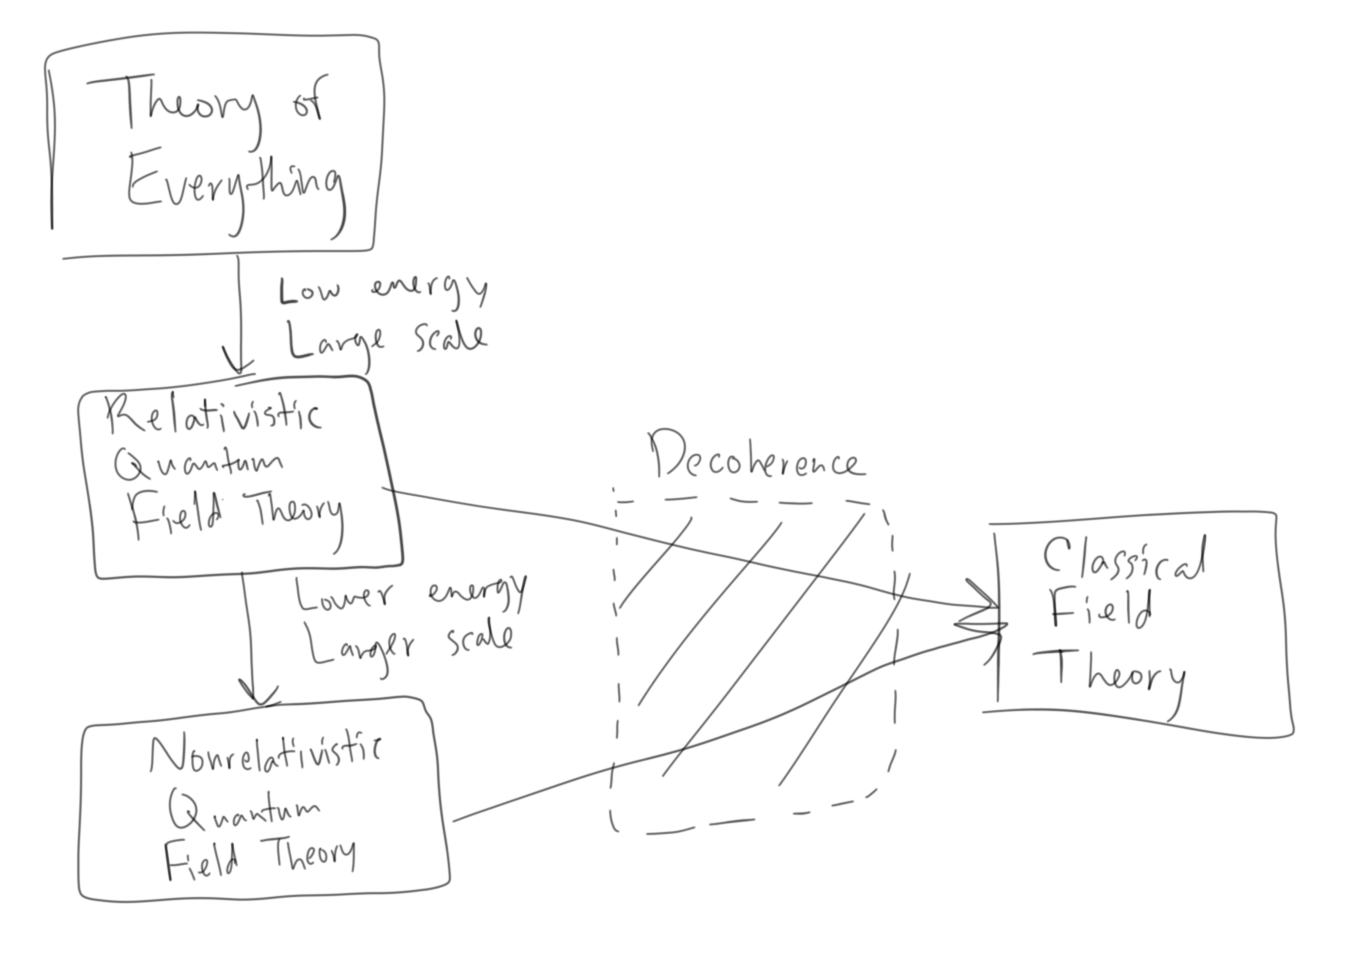
\includegraphics[width=\linewidth]{images/toe.png}
	\caption{Schematic of the study of field theories in physics.}
	\label{fig:fig1}
\end{figure}

\clearpage

\subsection*{Mathematical Machinery of Relativistic QFT}

For a quantum field theory to be relativistic it must be symmetric under the Poincar\'e group transformations.

\noindent Let the four-vector $(x_0, x_1, x_2, x_3)$ be the spacetime coordinates in an inertial reference frame. Then in any other reference frame that an observer chooses, the following condition is satisfied. 

\noindent (Note: We adopt the Einstein summation notation, and repeated indices are summed over, such that $\mu$, $\nu$, $\rho$, and $\sigma$ below are summed from $0$ to $3$.)

\begin{equation}
\eta_{\mu\nu} dx'^\mu dx'^\nu = \eta_{\rho\sigma} dx^\rho dx^\sigma
\end{equation}

\noindent Where we are using the Minkowski metric
\begin{equation}
\eta_{\mu\nu} 
= g_{\mu\nu} 
= \left( \begin{array}{rrrr} 
1 & 0 & 0 & 0 \\ 
0 & -1 & 0 & 0 \\ 
0 & 0 & -1 & 0 \\ 
0 & 0 & 0 & -1 
\end{array} \right)
.
\end{equation}

\noindent Any transformation satisfying the first equation, the relationship between the coordinates of two reference frames, must be a \textit{linear transformation} of the form, denoted by the pair $(\Lambda, a)$,
\begin{equation}
x'^\mu = \Lambda^\mu_{\,\,\,\nu} x^\nu + a^\mu
\end{equation}

\noindent Where $\Lambda^\mu_{\,\,\,\nu}$ is the $4x4$ Lorentz transformation matrix that represents rotations, and $a^\mu$ is a constant four-vector that represents spatial translations. 

\noindent Also note that the Lorentz transformation must satisfy the following condition, shown in index and matrix notation.
\begin{align}
	\eta_{\mu\nu} \Lambda^\mu_{\,\,\,\rho} \Lambda^\nu_{\,\,\,\sigma} &= \eta_{\rho\sigma} \\
	\Lambda^{T} \eta \Lambda &= \eta
\end{align}

\noindent These transformations $(\Lambda, a)$ are the elements of the Poincar\'e group $\mathcal{P}_4$. Let's check the group conditions, using equation \eqref{eq:eqn2} for calculating the product of two Poincar\'e transformations,

\begin{equation}
\begin{array}{llll} 
product & (\Lambda, a) \circ (\bar{\Lambda}, \bar{a}) & = & (\bar{\Lambda} \Lambda, \bar{\Lambda} a + \bar{a}) \\ 
identity & (1, 0) \circ (\Lambda, a) & = & (\Lambda, a) \\ 
inverse & (\Lambda^{-1}, a^{-1}) \circ (\Lambda, a) & = & (1, 0) \\ 
associativity & \left( (\Lambda, a) \circ (\bar{\Lambda}, \bar{a}) \right) \circ (\bar{\bar{\Lambda}}, \bar{\bar{a}}) & = & (\Lambda, a) \circ \left( (\bar{\Lambda}, \bar{a}) \circ (\bar{\bar{\Lambda}}, \bar{\bar{a}}) \right)
\end{array}
\end{equation}

\noindent In index notation, the total effect of the product of two Poincar\'e transfomations is written as
\begin{align}
x'^\mu &= \Lambda^\mu_{\,\,\,\nu} x^\nu + a^\mu \\
x''^\mu &= \bar{\Lambda}^\mu_{\,\,\,\rho} x'^\rho + \bar{a}^\mu
\end{align}

\noindent Quantum mechanical symmetries are representated by \textit{unitary} or \textit{anti-unitary} linear operators as elements of a separable Hilbert space $\mathscr{H}$ such that for each Poincar\'e transformation $(\Lambda, a) \in \mathcal{P}_4$, there exists a unitary transformation 
\begin{equation}
U(\Lambda, a) : \mathscr{H} \rightarrow \mathscr{H}
\end{equation}

\noindent The identity unitary transformation, and the product of any two unitary transformations of elements of the Poincar\'e group are physically indistinguishable from each other up to a phase factor $e^{i\phi}$, where $\phi \in \mathbb{R}$
\begin{align}
U(\bar{\Lambda}, \bar{a}) U(\Lambda, a) &= e^{i\phi((\Lambda, a),(\bar{\Lambda}, \bar{a}))} U(\bar{\Lambda} \Lambda, \bar{\Lambda} a + \bar{a}) \\
U(\mathbbm{1}, 0) &= e^{i\phi} \mathbbm{1} .
\end{align}

\noindent The family of transformations $U(\Lambda, a)$ that satisfy these equations is called the \textit{projective unitary representations of} $\mathcal{P}_4$, and is precisely what we need to establish a relativistic quantum field theory that includes translations, rotations, and Lorentz boosts as its transformations.\\

\noindent Consider the \textit{time translation subgroup} of the Poincar\'e group 
\begin{equation}
\{ (\Lambda=\mathbbm{1}, a=(t, 0, 0, 0)): t \in \mathbb{R} \} \subset \mathcal{P}_4
\end{equation}
\noindent And let $U$ be a unitary representation of $\mathcal{P}_4$. Then $V(t) = U(\mathbbm{1}, (t, 0, 0, 0))$ is a one-parameter family of unitary transformations, which is a group homomorphism, such that $V(s)V(t)=V(s+t)$, and is called a \textit{propagator}, and is a solution to the Schr\"{o}dinger equation, assuming the Hamiltonian $\hat{H}$ is self-adjoint and is stable, such that there at most a finite number of, preferrably zero, negative eigenvalues

\begin{equation}
\frac{d V(t)}{dt} = i \hat{H} V(t).
\end{equation}

\noindent So, having a unitary representation is equivalent to solving the time-dependent Schr\"{o}dinger equation, and we require that $U(\Lambda, a)$ is positive energy, such that the spectrum of eigenvalues of $\hat{H}$ is positive $spec(\hat{H}) \subset \mathbb{R}^+$, and stable. Otherwise, the system may be unstable and plunge to more and more negative eigenvalues. \\

\noindent All single-particle unitary representations of $\mathcal{P}_4$ have been classified by Wigner, and are labelled by their mass $m$ (invariant under Poincar\'e and Lorentz transformations) and their helicity/spin $s$. The bad news is that the universe is comprised of many particles, creating tension between locality and interactions, rendering thorough study of single-particle representations pointless. Even for a single particle, as we increase locality, self-interaction increases, and new particles are created via tunnelling. \\

\subsection*{Why is Obtaining a Relativistic Quantum Field Theory Hard?}

\noindent The reason that constructing a relativistic QFT is considered so difficult is because there are no nontrivial, only trivial, finite-dimensional unitary representations of the Poincar\'e group $\mathcal{P}_4$. The only nontrivial representations of $\mathcal{P}_4$ are infinite-dimensional, and are not easy to work with when constructing a unitary representation. Consider this in contrast to the, more easily constructed, special orthogonal group of three-dimensional rotations $SO(3)$ with unitary representations 

\begin{equation}
U = e^{i(\sigma_x \hat{J}_x + \sigma_y \hat{J}_y + \sigma_z \hat{J}_z)}. 
\end{equation}

\noindent Where $\hat{J}_\alpha$ are the angular momentum operators. The reason $SO(3)$ is easier to work with and construct a unitary representation is because $SO(3)$ a \textit{compact} group, while $\mathcal{P}_4$ is a \textit{non-compact} group.

\clearpage

\section{Lecture 2: Introduction to Classical Field Theory}
\label{sec: lec2}

\noindent To build a relativistic QFT, we start with an effective model from a \textit{classical field theory}, and make an "educated guess" to quantize the classical field theory. The desired relativistic QFT has nothing to do \textit{a priori} with the classical field theory. After quantization, the "educated guess", we take the limits of low energy, large scale, and decoherence, and check that we get back the classical field theory we started with, demonstrating whether the chosen quantization is correct or incorrect... enough, to some level of approximation.

\subsection*{Fields}

\noindent A \textit{field} is a quantity (e.g., density, spin, charge) tht is defined at every point on a manifold $\mathcal{M}$. Note that a rigorous definition of a field requires the introduction of vector bundles, of which we will not go so far. \\
We work on the Minkowski spacetime manifold $\mathcal{M} = \mathcal{M}_{1,3} = \mathbb{R}^1 \times \mathbb{R}^3$, with the field often taken to be two-times differentiable such that $\phi \in C^2(\mathcal{M}, \rho)$ and defined as a function from the manifold to some target space $\rho$
\begin{equation}
\phi : \mathcal{M} \rightarrow \rho 
\end{equation}

\noindent Some target spaces $\rho$, their associated field type, and example applications and models include

\begin{itemize}
\item $\rho = \mathbb{R}$; \textbf{scalar field}; charge density, magnetization density, Higgs boson
\item $\rho = \mathbb{R}^n$; \textbf{vector field}; electromagnetic field (actually a gauge field), pions
	\begin{figure}[H]
		\centering
		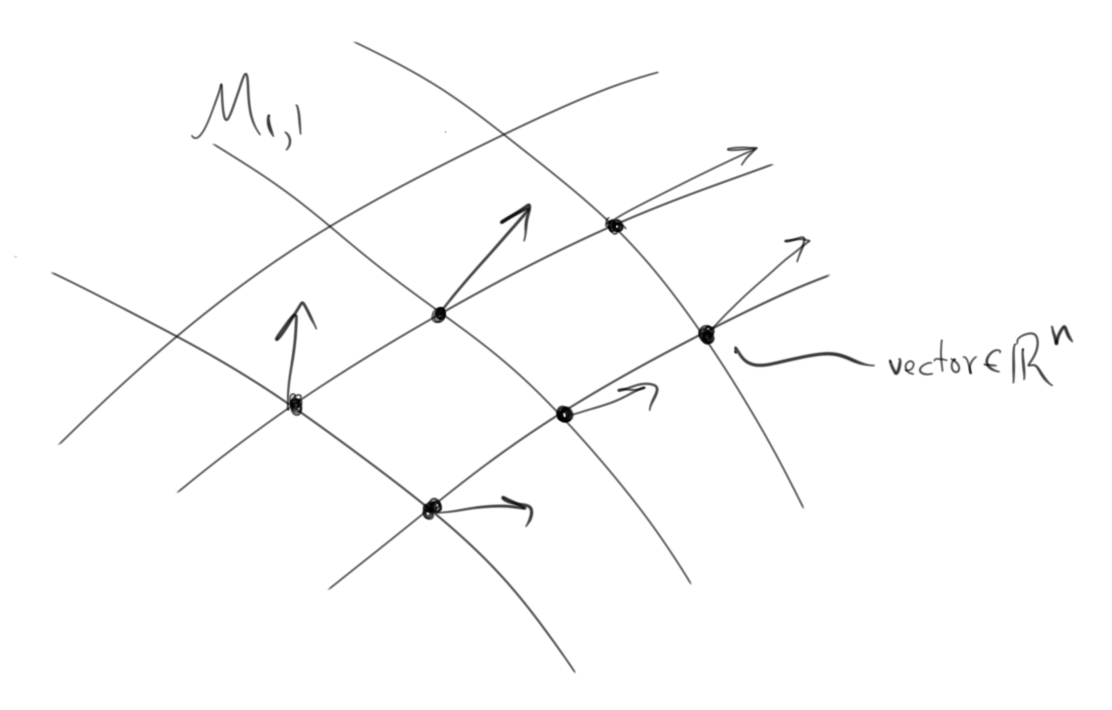
\includegraphics[scale=0.25]{images/vectorfield.png}
		\caption{Sketch of the vector field $\rho = \mathbb{R}^n$ over the Minkowski space $\mathcal{M}_{1,1}$.}
		\label{fig:fig1}
	\end{figure}
\item $\rho = \mathcal{S}^2$;  \textbf{vector field on the surface of a sphere};  $\sigma$-model, quantum magnets
\item $\rho = \mathcal{S}^1 \times \mathcal{S}^1$; \textbf{vector field on a torus}; Chern-Simons theory, Lie groups
\end{itemize}

\noindent Note that when our target space is the $N$-dimensional real vector field $\mathbb{R}^N$, the vector field is described as a list $N$ scalar fields $\{\phi_a(x)\}_{a=1}^N$, where $x$ is the coordinate four-vector.

\subsection*{Dynamics of Classical Fields}

\noindent We restrict this to discussion to classical dynamics generated by Lagrangians, obtained via the variational principle applied to th action functional, where the system of scalar fields $\{\phi_a(x)\}_{a=1}^N$, and $a$ labels the particle type (e.g., charge). The action functional $\mathcal{S}$ contains a function of the Langrangian density $\mathscr{L} = \mathscr{L}(\phi_a, \partial_\mu \phi_a)$. The Lagrangian density is actually a function of higher order derivatives of the fields $\phi_a$, but we make the assumption and approximation of first order derivatives, based on observation
\begin{equation}
\mathcal{S}(\Omega) = \int_\Omega d^4 x \,\, \mathscr{L}(\phi_a, \partial_\mu \phi_a). 
\end{equation}

\noindent Where $d^4 x = dx_0 dx_1 dx_2 dx_3$ and $\Omega \subset \mathcal{M}_{1,3}$, as a measurable set, is a region in $(3+1)$-dimensional spacetime. Typically, we consider the spacetime region as the entire Minkowski space $\Omega = \mathcal{M}_{1,3}$. \\

\noindent To extract the equations of motion, we suppose that the action $\mathcal{S}$ is stationary under infinitesimal variations of the component scalar fields $\phi_a(x) \rightarrow \phi_a(x) + \delta \phi_a(x)$, which vanish on the spacetime region boundary, such that $\delta\phi_a(x) = 0$ on $\partial\Omega$.  \\

\noindent Varying the action functional, we obtain $N$ \textit{Euler-Lagrange equations of motion}
\begin{align}
	\delta \mathcal{S} ( \Omega ) &= \int_\Omega d^4 x \,\, \left( \frac{\partial \mathscr{L}}{\partial \phi_a} \delta \phi_a + \frac{\partial \mathscr{L}}{\partial ( \partial_\mu \phi_a )} \delta ( \partial_\mu \phi_a ) \right) \\
	0 &= \int_\Omega d^4 x \,\, \left( \frac{\partial \mathscr{L}}{\partial \phi_a} \delta \phi_a - \frac{\partial}{\partial x^\mu} \left( \frac{\partial \mathscr{L}}{\partial ( \partial_\mu \phi_a )} \right) \right) \delta\phi_a + \int_\Omega d^4 x \,\, \frac{\partial}{\partial x^\mu} \left( \frac{\partial \mathscr{L}}{\partial ( \partial_\mu \phi_a )} \delta \phi_a \right) \\
	0 &= \int_\Omega d^4 x \,\, \left( \frac{\partial \mathscr{L}}{\partial \phi_a} \delta \phi_a - \frac{\partial}{\partial x^\mu} \left( \frac{\partial \mathscr{L}}{\partial ( \partial_\mu \phi_a )} \right) \right) \delta\phi_a + \partial_\mu \mathcal{M}^\mu.
\end{align}

\noindent The last term is a surface term which vanishes on the boundary, since we first demanded that $\delta\phi_a = 0$ vanishes on the boundary, such that $\partial_\mu \mathcal{M}^\mu = 0$ on $\partial\Omega$. \\

\noindent Since $\mathcal{S}(\Omega)$ is stationary with respect to all variations of the fields $\delta\phi_a$ and admissable spacetime regions $\Omega$, the integrand of the remaining term must also vanish $\forall \, a = 1, 2,... \, , N$, and we obtain the $N$ Euler-Lagrange equations of motion
\begin{equation}
-\frac{\partial \mathscr{L}}{\partial \phi_a} + \frac{\partial}{\partial x^\mu} \left( \frac{\partial \mathscr{L}}{\partial (\partial_\mu \phi_a)} \right) = 0.
\end{equation}

\noindent So, with equations of motion in hand, gotten by whatever means, they can be encoded in the Langrangian density, and then recovered via the Euler-Lagrange equations of motion. This allows us to discover equations of motion with certain properties, such as being symmetric under the Poincar\'e transformations, by designing Lagrangian densities, which are scalars under these symmetry transformations, apply Euler-Lagrange "recipe", and get the equations of motion, which are guaranteed to be symmetric under the chosen transformations. This benefit of the action principle makes it easy to design equations of motion with certain symmetries. \\

\subsection*{Example: Klein-Gordon field}

Consider the Langrangian density 
\begin{align}
\mathscr{L} &= \frac{1}{2}\dot{\phi}^2 - \frac{1}{2}(\nabla\phi)^2 - \frac{1}{2}m^2\phi^2 \\
&= \frac{1}{2}(\partial_\mu \phi)^2 - \frac{1}{2}m^2\phi^2
\end{align}

\noindent Where $\dot{\phi} = \partial_0 \phi$ is the time derivative of the field, and $(\nabla\phi)_j = \partial_j\phi$ for $j=1, 2, 3$ are the $x$, $y$, $z$ spatial components of the field derivatives. \\

\noindent Apply the Euler-Lagrange equations of motion to obtain the dynamics of the Klein-Gordon field
\begin{align}
-\frac{\partial \mathscr{L}}{\partial \phi_a} + \frac{\partial}{\partial x^\mu} \left( \frac{\partial \mathscr{L}}{\partial (\partial_\mu \phi_a)} \right) &= 0 \\
\frac{\partial}{\partial x^\mu}(\partial^\mu \phi) -(-m^2 \phi) &= 0 \\
\partial_\mu \partial^\mu \phi + m^2 \phi &=0 \\
\Box \phi + m^2 \phi &= 0
\end{align}

\subsection*{Hamiltonian formalism}

\noindent A better way to guess/build a quantum theory, with the correct calssical limit determined by the Langrangian density, is the \textit{Hamiltonian formalism}, where we calculate conjugate variables and impose canonical (algebraic) commutation relations. \\

\noindent Suppose that $\phi_a(x)$ is a component field's \textit{canonical position}. Then define the \textit{conjugate momentum density} for each field to be 
\begin{equation}
\pi_a(x) = \frac{\partial \mathscr{L}}{\partial \dot{\phi_a}}.
\end{equation}

\noindent In order to computationally study a field, we discretize the space into a regular lattice with spacing $\epsilon$ between each lattice site, since representing a continuous object on a computer would require an infinite amount of data. Discretization yields generalized coordinates, defined by the field itself, of the form $q_j^a(t) = \phi_a(t, x_j), \, j \in \mathbb{Z}$. For example, consider the $1+1$-dimensional Minkowski space $\mathcal{M}_{1,1}$

\begin{figure}[H]
	\centering
	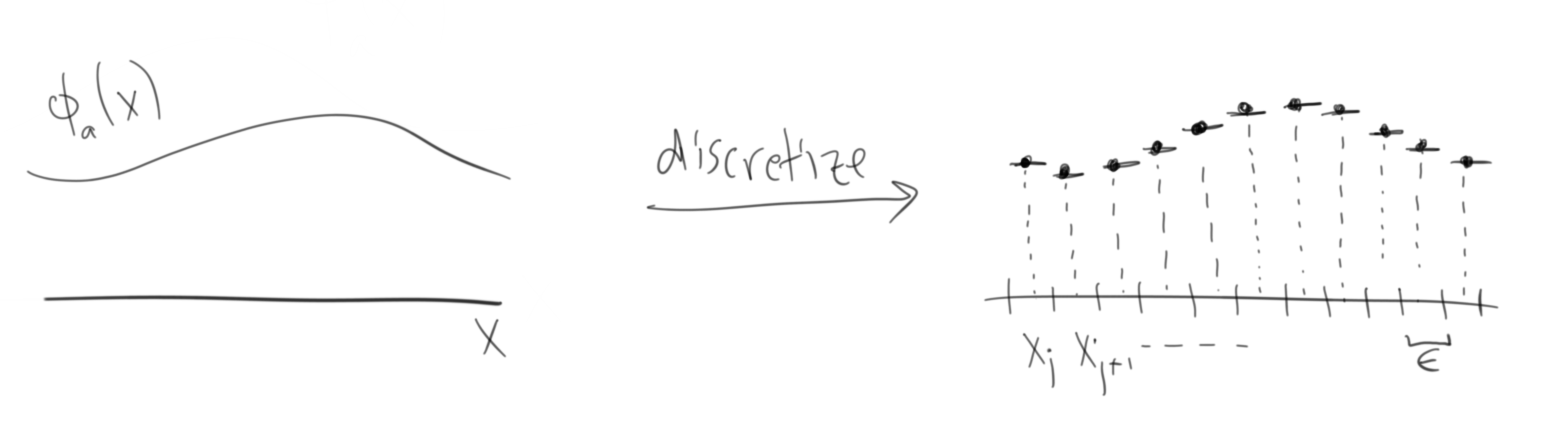
\includegraphics[width=\linewidth]{images/discrete.png}
	\caption{Schematic of field discretization.}
	\label{fig:fig3}
\end{figure}

\noindent To discretize the action functional and apply the variational principle, replace the partial derivatives $\partial_\mu \phi_a(t, x)$, since it is a continuous operation, by applying Taylor's theorem to approximate the spatial component of the field as a finite difference, where $\epsilon$ should be made as small as possible such that the error approximation is minimized
\begin{equation}
\partial_x \phi_a(t, x_j) \cong \frac{\phi_a(t, x_j + \epsilon) - \phi_a(t, x_j)}{\epsilon} = \frac{q^a_{j+1} - q^a_j}{\epsilon}.
\end{equation}

\noindent Leave the temporal component to be continuous
\begin{equation}
\partial_t \phi_a(t, x_j) \cong \dot{q}_j^a . 
\end{equation}

\noindent To obtain the Lagrangian, integrate the density over space, such that only the time dependence is left
\begin{equation}
\int d^3 x \,\, \mathscr{L} (\phi_a, \partial_\mu \phi_a) = L(q_j^a (t), \dot{q}_j^a (t)) = L(t) . 
\end{equation}

\noindent The discrete approximation of the Lagrangian is written as 
\begin{equation}
L(t) \cong \sum_j \delta x_j \mathscr{L}(\phi_a(t, x_j), \partial_\mu \phi_a(t, x_j)). 
\end{equation}

\noindent And the discrete conjugate momenta 
\begin{equation}
p_j^a(t) = \frac{\partial L}{\partial \dot{q}_j^a} = \sum_j \delta x_j \frac{\partial \mathscr{L}}{\partial \dot{q}_j^a} = \sum_j \delta x_j \pi^a(t, x_j).
\end{equation}

\subsubsection*{Simple Example}

\noindent As a simple example, consider the Lagrangian density 
\begin{align}
\mathscr{L} &= \frac{1}{2} (\partial_\mu \phi \partial^\mu \phi) \\
&= \frac{1}{2}(\partial_t \phi)^2 - \frac{1}{2} (\partial_x \phi)^2 .
\end{align}

\noindent (RECHECK) Integrate over space $d^3 x$ to obtain the Lagrangian, and discretize using the rules defined above
\begin{equation}
L(t) = \frac{1}{2} \sum_{j=-\infty}^{\infty} \left( \epsilon \left( \frac{d q_j}{d t} \right)^2 - \frac{(q_{j+1} - q_j)}{\epsilon} \right) .
\end{equation}

\noindent Where $\delta x_j = \epsilon$ and $p_j(t) = \epsilon \frac{d q_j}{dt} = \pi(t, x_j) \delta x_j $. 

\noindent As $\epsilon \rightarrow 0$, $q_j(t) \rightarrow \phi(t, x)$ and $p_j(t) \rightarrow \dot{\phi(t, x)}$

\subsubsection*{Hamiltonian Density}

\noindent For the discrete approximation, the Hamiltonian $H$, obtained by integrating the Hamiltonian density $\mathscr{H}$ of space $d^3 x$, is written as 
\begin{equation}
H = \sum_j p_j^a \dot{q}_j^a - L = \sum_j \delta x_j ( \pi_a(t, x_j) \dot{\phi}_a(t, x_j) - \mathcal{L}_j )
\end{equation}

\noindent In the limit as $\epsilon \rightarrow 0$, the Hamiltonian density is 
\begin{equation}
\mathscr{H}(t, x) = \pi_a(t, x) \dot{\phi}_a(t, x) - \mathscr{L} \left( \phi_a(t, x), \partial_\mu \phi_a(t,x) \right)
\end{equation}

\noindent The Hamiltonian density for the Klein-Gordon field is, dropping the field index and spacetime dependencies from the expression, 
\begin{equation}
\mathscr{H} = \frac{1}{2}\pi^2 + \frac{1}{2}(\nabla \phi)^2 + \frac{1}{2} m^2 \phi^2
\end{equation}

\clearpage

\section{Lecture 3: Symmetries in Classical Field Theory}
\label{sec: lec3}

\noindent Suppose that $\mathscr{L}(\phi_a, \partial_\mu \phi_a)$ is the Lagrangian density for some set of fields $\{ \phi_a(x) \}_{a=1}^N$. Recall that the Lagrangian density is a compact, encrypted of writing the equations of motion of a system, and the Euler-Lagrange equations and the principle of least action are used to unpack/decrypt the equations of motion. \\

\noindent Now consider an infinitesimal continuous transformation of the fields
\begin{equation}
\phi_a '(x) = \phi_a(x) + X_a(\phi_a)
\end{equation}

\noindent This produces an \textit{infinitesimal symmetry} in the equations of motion when they are left invariant under the principle of least action
\begin{align}
\mathscr{L} &\rightarrow \mathscr{L}(\phi_a', \partial_\mu \phi_a') = \mathscr{L}(\phi_a, \partial_\mu \phi_a) + \partial_\mu F^\mu \\
\& \,\,\,\, \mathcal{S} [ \phi_a ] &= \int d^4 x \mathscr{L} = \int d^4 x ( \mathscr{L} + \partial_\mu F^\mu )
\end{align}

\subsection*{Noether's Theorem}

\noindent Every continuous symmetry of a Lagrangian implies the existence of a conserved current $j^\mu(x)$. \\

\noindent \textbf{Proof:} Let $X_a[\phi_a] = \delta \phi_a$ be an arbitrary, infinitesimal change in each field, such that the infinitesimal change in the Lagrangian density is 

\begin{align}
\delta \mathscr{L}(\phi_a, \partial_\mu \phi_a) &= \mathscr{L}(\phi_a+\delta \phi_a, \partial_\mu(\phi_a + \delta \phi_a)) - \mathscr{L}(\phi_a, \delta_\mu \phi_a) \\
&\cong \frac{\partial \mathscr{L}}{\partial \phi_a} \delta \phi_a + \frac{\partial \mathscr{L}}{\partial (\partial_\mu \phi_a)} \delta(\partial_\mu \phi_a) \\
&= \left( \frac{\partial \mathscr{L}}{\partial \phi_a} - \partial_\mu \left( \frac{\partial \mathscr{L}}{\partial (\partial_\mu \phi_a)} \right) \right) \delta \phi_a + \partial_\mu \left( \frac{\partial \mathscr{L}}{\partial (\partial_\mu \phi_a)} \delta \phi_a \right) \\
\delta \mathscr{L}(\phi_a, \partial_\mu \phi_a) &= \partial_\mu \left( \frac{\partial \mathscr{L}}{\partial (\partial_\mu \phi_a)} \delta \phi_a \right)
\end{align}

\noindent Where in line $(14)$, we have kept only first order terms $\mathcal{O} (\delta \phi_a)$, and have used the Taylor expansion and added zero to get to line $(15)$. To obtain line $(16)$, note that the first term in line $(15)$ is equal to zero, since $\phi_a(x)$ obey the Euler-Lagrange equations. \\

\noindent As defined above, for an infinitesimal transformation, call $\delta \phi_a = X_a[\phi_a]$  and  for an infinitesimal symmetry, call $\delta \mathscr{L} = \partial_\mu F^\mu$.

\begin{align}
\partial_\mu F^\mu &= \partial_\mu \left( \frac{\partial \mathscr{L}}{\partial (\partial_\mu \phi_a)} X_a[\phi_a] \right) \\
0 &= \partial_\mu \left( \frac{\partial \mathscr{L}}{\partial (\partial_\mu \phi_a)} X_a[\phi_a] - F^\mu \right)
\end{align}

\noindent Call the conserved quantity the conserved current 
\begin{equation}
j^\mu (x) = \left( \frac{\partial \mathscr{L}}{\partial (\partial_\mu \phi_a)} X_a[\phi_a] - F^\mu \right).
\end{equation}

\noindent Now, a conserved current implies the existence of a conserved charge. For any measurable region in our Minkowski space $V \subset \mathcal{M}$, define the integral of the time-like component of the current as
\begin{equation}
Q_V = \int_V d^3 x \,\, j^0(x)
\end{equation}

\noindent Take $V=\mathbb{R}^3$, and assume that the current vanishes at infinity, such that $j \rightarrow 0$ on the boundary $\partial V$, and take the time derivative
\begin{align}
\frac{d Q_{\mathbb{R}^3}}{d t} &= \int_{\mathbb{R}^3} d^3x \,\, \partial_0 j^0 (x) \\
&= - \int_{\mathbb{R}^3} d^3x \,\, \partial_k j^k \\
&= - \int_{\partial \mathbb{R}^3} j  ds \\
\frac{d Q_{\mathbb{R}^3}}{d t} &= 0
\end{align}

\subsection*{Example}

\noindent Consider an active transformation of spacetime coordinates $x^\mu \rightarrow x^\mu - \epsilon^\mu$.

\noindent Then each field transforms as
\begin{align}
\phi'_a(x^\mu) &= \phi_a(x^\mu + \epsilon^\mu) \\
&= \phi_a(x^\mu) + \epsilon^\nu \partial_\nu \phi_a(x^\mu)
\end{align}

\noindent And the Lagrangian density transforms as, yielding $4 \times 4=16$ equations from summing over $\mu$ and $\nu$ 
\begin{align}
\mathscr{L}(x'^\mu) &= \mathscr{L} (x^\mu + \epsilon^\mu) \\
&= \mathscr{L}(x^\mu) + \epsilon^\nu \partial_\nu \mathscr{L}(x^\mu)
\end{align}

\noindent Where the infinitesimal field transformation is $X_a[\phi_a] = \epsilon^\nu \partial_\nu \phi_a(x^\mu)$, and the infinitesimal symmetry of the Lagrangian density is $\partial_\mu F^\mu = \epsilon^\mu \partial_\mu \mathscr{L}(x^\mu)$ \\

\noindent Consider the infinitesimal element $\epsilon$ with basis vector entries $[\hat{\nu}]^\mu_{\,\,\,\nu} = \delta^\mu_{\,\,\,\nu}$
\begin{equation}
\epsilon^\mu = \epsilon \hat{\nu}^\mu = \epsilon \{ (1,0,0,0), (0,1,0,0), (0,0,1,0), (0,0,0,1) \}.
\end{equation}

\noindent Apply Noether's theorem to each of the 4 symmetry terms $\epsilon \hat{\nu}^\mu$, yielding 16 total terms that we assign as the elements $T^\mu_{\,\,\,\nu}$ of the \textit{energy-momentum} or \textit{stress-energy tensor}
\begin{align}
T^\mu_{\,\,\,\nu} = j^\mu_{\,\,\,\nu} = \frac{\partial \mathscr{L}}{\partial (\partial_\mu \phi_a)} \partial_\nu \phi_a - \delta^\mu_{\,\,\,\nu} \mathscr{L}.
\end{align}

\noindent Note that each of the $\nu^{th}$ columns of the energy-momentum tensor correspond to one of the four conserved currents and translation in each of the $\nu^{th}$ directions
\begin{align}
\partial_\mu T^\mu_{\,\,\,\nu} = 0, \,\,\,\, \forall \,\, \nu.
\end{align}

\noindent In a \textit{closed} system, the corresponding conserved charges, from the columns (conserved currents) of the energy-momentum tensor, are the total energy and the momentum in each of the three spatial directions
\begin{align}
E &= \int d^3x \,\,\, T^{00} \\
p^j &= \int d^3x \,\,\, T^{0j} .
\end{align}

\subsubsection*{Example of the Example: Klein-Gordon Field}

Consider the Klein-Gordon Lagrangian density $\mathscr{L} = \frac{1}{2} \partial_\mu \phi \partial^\mu \phi - \frac{1}{2}m^2 \phi^2$. The energy-momentum tensor has elements of the form
\begin{align}
T^\mu_{\,\,\,\nu} &= \partial^\mu \phi \partial_\nu \phi - \delta^\mu_{\,\,\,\nu}\mathscr{L} \\
T^{\mu \nu} &= \eta^{\nu \nu'} T^\mu_{\,\,\,\nu'} = \partial^\mu \phi \partial^\nu \phi - \eta^{\mu \nu} \mathscr{L}.
\end{align}

\noindent The corresponding conserved charges are
\begin{align}
E &= \int d^3x \,\, \mathscr{H}(x) = \int d^3x \,\, (\partial^0 \phi \partial^0 \phi - \frac{1}{2}\partial^0 \phi \partial^0 \phi + \frac{1}{2} m^2 \phi^2) \\
p^j &= \int d^3x \,\, \dot{\phi} \partial^j \phi .
\end{align}

\subsubsection*{How To Apply Noether's Theorem}
\begin{enumerate}
\item Identify the continuous symmetry. \\
\item Calculate the change in the Lagrangian density. \\
\item Calculate the change in each of the fields. \\
\item Work out the conserved currents and charges.
\end{enumerate}

\subsection*{Infinitesimal Lorentz Transformations}

\noindent Consider the transformation $x^\mu \rightarrow \Lambda^\mu_{\,\,\,\nu} x^\nu$, where $\Lambda^\mu_{\,\,\,\nu} = \delta^\mu_{\,\,\,\nu} + \omega^\mu_{\,\,\,\nu}$, and $\omega^\mu_{\,\,\,\nu}$ is infinitesimal. Next, recall the following property of the group of Lorentz transformations, restricting the possible values for $\omega$
\begin{align}
\eta &= \Lambda^T \eta \Lambda \\
\eta^{\mu \nu} &= (\delta^\mu_{\,\,\,\sigma} + \omega^\mu_{\,\,\,\sigma} ) (\delta^\nu_{\,\,\,\tau} + \omega^\nu_{\,\,\,\tau} ) \eta^{\sigma \tau} \\
0 &=_{\mathcal{O}(\omega)} \omega^{\mu \nu} + \omega^{\nu \mu}
\end{align}

\noindent This is a linear equation in $\omega$, since we have kept only up to first order terms in $\omega$, and tells us that $\omega$ is an \textit{antisymmetric}, infinitesimal generator of Lorentz transformations with six independent variables which define six continuous symmetries and six conserved currents and charges.

\begin{equation}
\omega = \left(
\begin{array}{cccc}
0 & -\alpha & -\beta & -\gamma \\
\alpha & 0 & -\delta & -\epsilon \\
\beta & \delta & 0 & -\kappa \\
\gamma & \epsilon & \kappa & 0 \\
\end{array}
\right)
\end{equation}

\noindent The action of this infinitesimal Lorentz transformation on the fields is 
\begin{align}
\phi_a(x) \rightarrow \phi'_a(x) &= \phi_a(\Lambda^{-1}x) \\
&= \phi_a((\delta-\omega)x) \\
&= \phi_a(x^\mu - \omega^\mu_{\,\,\,\nu} x^\nu) \\ 
&=_{\mathcal{O}(\omega)} \phi_a(x) - \omega^\mu_{\,\,\,\nu} x^\nu \partial_\mu \phi_a(x)
\end{align}

\noindent Showing that the symmetry is defined by the infinitesimals
\begin{align}
\delta \phi_a &= -\omega^\mu_{\,\,\,\nu} x^\nu \partial_\mu \phi_a \\
\& \,\,\,\, \delta \mathscr{L} &= -\omega^\mu_{\,\,\,\nu} x^\nu \partial_\mu \mathscr{L} = -\partial_\mu(\omega^\mu_{\,\,\,\nu} x^\nu \mathscr{L}) \\
\& \,\,\,\, j^\mu_{\,\,\,\omega} &= \frac{\partial \mathscr{L}}{\partial (\partial_\mu \phi_a)} \omega^\rho_{\,\,\,\nu} x^\nu \partial_\rho \phi_a + \omega^\mu_{\,\,\,\nu} x^\nu \mathscr{L}.
\end{align}

\noindent (CHECK how $j$ to $\mathcal{J}$) Applying Noether's theorem tells us that the six independent conserved currents $\partial_\mu (\mathcal{J}^\mu)^{\rho \sigma} = 0$, and conserved charges, are of the form
\begin{align}
(\mathcal{J}^\mu)^{\rho \sigma} &= x^\rho T^{\mu \sigma} - x^\sigma T^{\mu \rho} \\ 
Q^{jk} &= \int d^3x \,\, (x^j T^{0k} - x^k T^{0j}) \\
Q^{0j} &= \int d^3x \,\, (x^0 T^{0j} - x^j T^{00})
\end{align}

\noindent Call $Q^{jk}$ the generators of rotations, and $Q^{0j}$ the generators of boosts of the Lorentz transformations.

\subsection*{Generators}

\noindent Let $f$ and $g$ be maps from phase space to the real numbers 
\begin{equation}
f, \, g: \,\, \mathbb{R}^N \times \mathbb{R}^N \rightarrow \mathbb{R}.
\end{equation}

\noindent Define the Poisson bracket with the pairs of canonical coordinates $(q_j, p_j)$
\begin{align}
\{f,g\} &= \sum_{j=1}^N \left( \frac{\partial f}{\partial q_j} \frac{\partial g}{\partial p_j} - \frac{\partial f}{\partial p_j} \frac{\partial g}{\partial q_j} \right) \\
\{f, H \} &= \frac{d f}{d t}
\end{align}

\noindent The field theory version of the Posson bracket is defined with the canonical coordinate pairs $(\phi(x), \pi(x))$
\begin{align}
\{F, G\} &= \int d^3x \,\, \left( \frac{\delta F}{\delta \phi(x)} \frac{\delta G}{\delta \pi(x)} - \frac{\delta F}{\delta \pi(x)} \frac{\delta G}{\delta \phi(x)} \right) \\
\{f, Q^{\rho \sigma}\} &= \frac{\partial f}{\partial s^{\rho \sigma}}
\end{align}

\noindent Where the Poisson bracket of $f$ and the conserved charges $Q$ generate the corresponding symmetry transformations. Conserved cahrges also obey the Lie algebra obeyed by the Poincar\'e group.

\subsection*{Standard Dogma of Quantization}

\noindent Basically, put hats on things

\begin{itemize}
\item Function $f$ on phase space $\rightarrow$ linear operator $\hat{f}$ (observable) on Hilbert space \\
\item Poisson bracket $\{ f,g \} = h \rightarrow$ commutator $[\hat{f}, \hat{g}] = i \hat{h}$ \\
\item Conserved charge $Q^{\rho \sigma} \rightarrow$ conserved charge operator $\hat{Q}^{\rho \sigma}$
\end{itemize}

\noindent Where the conserved charge operators generate the Lorentz transformations on Hilbert space
\begin{equation}
\frac{d \hat{U}}{d s} = i [\hat{U}, \hat{Q}^{\rho \sigma}] \omega_{\rho \sigma}
\end{equation}

\clearpage

\section{Lecture 4: Field Quantization}
\label{sec:lec4}

\noindent More than one quantum field theory can have the same classical field theory as an effective model, making field quantization not a well-posed problem. Developing a quantum field theory is therefore built on educated guesses.

\subsection*{Canonical quantization of particles} 
 
\noindent The standard approach of \textit{canonical quantization} is to begin with a classical theory and suppose $n$ classical degrees of freedom, which are used to measure the canonical coordinate pairs, \textit{position} $q_j$ and \textit{momentum} $p_j$, for each degree of freedom, such that the Poisson bracket is defined by $\{q_j, p_k \} = \delta_{jk}$. The total energy of the of the system is measured by the classical \textit{Hamiltonian}, defined by 
\begin{equation}
H = \sum_{j=1}^n \frac{p_j^2}{2 m} + \frac{m}{2} \sum_{j, k=1}^n q_j [\textbf{Q}]_{jk} q_k
\end{equation}

\noindent Where $\textbf{Q}$ is an $n \times n$ symmetric, positive matrix. \\

\noindent For example, consider the quantum harmonic oscillator, and take the naive approach by basically putting hats on everything. This ends up working for field quantization, and yields a unitary representation of the Poincar\'e group. \\

\begin{itemize}
\item \textbf{Canonical coordinates}: $(q_j, p_j) \\ \rightarrow \textbf{Canonical coordinate operators}: (\hat{q}_j, \hat{p}_j)$ \\
\item \textbf{Poisson bracket}: $\{ q_j, p_k \} = \delta_{jk}$ \\ $\rightarrow$ \textbf{Commutator}: $[\hat{q}_j, \hat{p}_k] = i \delta_{jk}$ \\
\item \textbf{Hamiltonian}: $H$, as defined above \\ $\rightarrow \textbf{Hamiltonian operator}: \hat{H} = \sum_{j=1}^n \frac{\hat{p}_j^2}{2 m} + \frac{m}{2} \sum_{j, k=1}^n \hat{q}_j [\textbf{Q}]_{jk} \hat{q}_k$
\end{itemize}

\noindent To diagonalize the Hamiltonian operator, first note that since $\textbf{Q}$ is a symmetric, positive $n \times n$ matrix, there exists an orthogonal matrix $\textbf{O}$ (s.t., $\textbf{O}^T \textbf{O} = \textbf{I}$), such that $\textbf{O} \textbf{Q} \textbf{O}^T = \textbf{D}$, where $\textbf{D}$ is a diagonal matrix, where we call the diagonal elements $\{ \omega_i^2 \}_{i=1}^n$ \\

\noindent Now, transform the canonical coordinates, using the orthogonal matrix, such that the correct commutation relation is still obeyed
\begin{align}
\hat{q}_j &= \sum_{k=1}^n [\textbf{O}]_{jk} \hat{q}'_k \\
\hat{p}_j &= \sum_{k=1}^n [\textbf{O}]_{jk} \hat{p}'_k \\
i \delta_{jk} &= [ \hat{q}'_j, \hat{p}'_k ]
\end{align}

\noindent Using the facts that $\textbf{O}^T = \textbf{O}^{-1}$ and $\textbf{O} \textbf{Q} \textbf{O}^T = \textbf{D}$, the Hamiltonian becomes diagonalized
\begin{align}
\hat{H} &= \sum_{j=1}^n \frac{\hat{p'}_j^2}{2 m} + \frac{m}{2} \sum_{j, k, l, m=1}^n \hat{q'}_l [\textbf{O}^T]_{jl} [\textbf{Q}]_{jk} [\textbf{O}^T]_{km} \hat{q'}_m \\
\hat{H} &= \sum_{j=1}^n \frac{\hat{p'}_j^2}{2 m} + \frac{1}{2} \sum_{k=1}^n \omega_k^2 \hat{q'}_k^2 \\
\hat{H} &= \frac{1}{2} \sum_{k=1}^n \omega_k (\hat{a}_k^\dagger \hat{a}_k + \frac{1}{2})
\end{align}

\noindent Where the annihilation and creation ladder operators that diagonalize the quantum harmonic oscillator Hamiltonian are defined as
\begin{align}
\hat{a}_k &= \sqrt{\frac{m \omega_k}{2}} (\hat{q}'_k + \frac{i}{m \omega_k} \hat{p}'_k) \\
\hat{a}_k^\dagger &= \sqrt{\frac{m \omega_k}{2}} (\hat{q}'_k - \frac{i}{m \omega_k} \hat{p}'_k)
\end{align}

\subsection*{Canonical Quantization of Fields}

\noindent To quantize the Klein-Gordon field, we follow the same seemingly naive approach of putting hats on everything. In this example fo quantizing a field, the continuous variable $x$ is used, in contrast to the discrete labels $j$ in the previous example of the quantum harmonic oscillator

\begin{itemize}
\item \textbf{Canonical coordinates}: $(\phi(x), \pi(x)) \\ \rightarrow \textbf{Canonical coordinate operators}: (\hat{\phi}(x), \hat{\pi}(x))$ \\
\item \textbf{Poisson bracket}: $\{ \phi(x), \pi(y) \} = \delta^{(3)}(x-y)$ \\ $\rightarrow$ \textbf{Commutator}: $[\hat{\phi}(x), \hat{\pi}(y)] = i \delta^{(3)}(x-y)$ \\
	\subitem Note that this is the \textit{equal time Poisson bracket}, such that $(x-y)$ is the spatial three-vector.
	\subitem Also note that this commutator is strange,  as it is comprised of "two self-adjoint operators and something's that not even a function" \\
\item \textbf{Hamiltonian}: $H_{KG} = \frac{1}{2} \int d^3x \,\, \left( \pi^2(x) + (\nabla \phi(x))^2 + \frac{1}{2} m^2 \phi^2(x) \right)$ \\ $\rightarrow \textbf{Hamiltonian operator}: \hat{H}_{KG} = \frac{1}{2} \int d^3x \,\, \left( \hat{\pi}^2(x) + (\nabla \hat{\phi}(x))^2 + \frac{1}{2} m^2 \hat{\phi}^2(x) \right)$
\end{itemize}

\noindent Essentially, replace discrete sums with continuous integrals, by switching to a continuous label $j \rightarrow x$ and a continuous dynamical variable $q_j \rightarrow q_x=\phi(x)$. Solving the quantum Hamiltonian, by analogy of the canonical quantization of particles, should be as simple as creating the analog of the $\textbf{Q}$ matrix and its diagonalization. \\

\noindent  Replacing sums by integrals allows the full diagonalization of $\textbf{Q}$, and, therefore, the full diagonalization of the Hamiltonian $\hat{H} = \hat{H}_{KG}$, but this does not yet yield a unitary representation of the Poincar\'e group or a valid relativistic quantum field theory. Diagonalizing the Hamiltonian only quantizes a one-parameter subgroup of the Poincar\'e group. The conserved currents, charges, and operators obeying the correct Lie algebra are still needed for a relativistic quantum field theory. \\

\subsubsection*{Diagonalization of the quantum field theory}

\noindent The diagonalization of a field theory begins with emergence of the \textit{Fourier transform}. Replace sums with integrals, and, since the matrix elements are described by two numbers, let's define a continuous function in two variables $K(x,y)$

\begin{equation}
\hat{q}_j = \sum_k [\textbf{O}]_{jk} \hat{q}'_k \,\,\,\, \rightarrow \,\,\,\, \hat{\phi}(x) = \int d^3 y \,\, K(x, y) \hat{\phi}(y)
\end{equation}

\noindent Where $K(x,y)$ is the \textit{kernel} of the Fourier transform. \\

\noindent Using the Fourier transform is motivated by certain features of symmetric matrices. Consider the \textit{circulant} matrix, a type of Toeplitz matrix where each successive column is a cyclic permutation of the previous column, initialized by the first column vector, and has the form as an $n \times n$ matrix 

\begin{equation}
\begin{bmatrix} 
 c_0 & c_{n-1} & \dots & c_2 & c_1 \\
 c_1 & c_0 & c_{n-1} &  & c_2 \\
 \vdots & c_1 & c_0 &  \ddots & \vdots \\
 c_{n-2} &  & \ddots &  \ddots & c_{n-1} \\
 c_{n-1} & c_{n-2} & \dots &  c_1 & c_0 
\end{bmatrix}.
\end{equation} \\

\noindent These matrices are diagonalized via the discrete Fourier transform, which is an $n \times n$ unitary matrix, though not orthogonal and may have complex entries

\begin{equation}
\textbf{U} = \frac{1}{\sqrt{n}} 
\begin{bmatrix} 
 1 & 1 & 1 & \dots &  \\
 1 & \mu & \mu^2 & \dots &  \\
 1 & \mu^2 & \mu^4 &   & \vdots \\
 \vdots & \vdots & &  \mu^{jk} &  \\
  &  & \dots &  & \mu^{nn} 
\end{bmatrix}
\end{equation}


\noindent Where $\mu = e^{\frac{2 \pi i}{n}}$ is the $n^{th}$ roots of unity. The elements of the discrete Fourier transform, therefore, have the form $\frac{1}{\sqrt{n}} e^{\frac{2\pi i j k}{n}}$. Compare this to the continuous Fourier transform kernel function $K(x,y) = \frac{1}{2\pi} e^{ixy}$. \\

\noindent For transformations between position and momentum space, make the guess that the Fourier transform that will diagonalize our quantized Klein-Gordon Hamiltonian has the form 

\begin{equation}
\hat{\phi}(x) = \int \frac{d^3 p}{(2\pi)^3} e^{i p \cdot x} \hat{\phi}_p(p).
\end{equation}

\noindent Where $\hat{\phi}_p(p)$ is the momentum space wavefunction, and is not Hermitian, such that $\hat{\phi}_p(p)^\dagger = \hat{\phi}_p(-p)$. To check if the guess is correct, apply $\hat{H}_{KG}$ to the transform defined above, and observe whether it is diagonalized or not. \\

\noindent As in the discrete case of diagonalization, we construct ladder operators

\begin{align}
\hat{\phi}(x) &= \int \frac{d^3 p}{(2 \pi)^3} \frac{1}{\sqrt{2 \omega_p}} \left( \hat{a}_p e^{ip \cdot x} + \hat{a}_p^\dagger e^{-ip \cdot x} \right) \\
\hat{\pi}(x) &=-i  \int \frac{d^3 p}{(2 \pi)^3} \sqrt{\frac{\omega_p}{2}} \left( \hat{a}_p e^{ip \cdot x} - \hat{a}_p^\dagger e^{-ip \cdot x} \right) \\
&\omega_p = \sqrt{ |p|^2 + m^2}
\end{align}

\noindent Check the commutation relation
\begin{align}
[ \hat{\phi}(x), \hat{\pi}(x') ] &= \frac{-i}{2} \int \frac{d^3 p d^3 p'}{(2 \pi)^6} \sqrt{\frac{\omega_{p'}}{\omega_p}} \left( [\hat{a}_{-p}^\dagger, \hat{a}_{p'}] - [\hat{a}_p, \hat{a}_{-p'}^\dagger] \right) e^{i(p \cdot x+p' \cdot y)} \\
& \,\,\,\, \,\,\,\, \,\,\,\, \,\,\,\, \,\,\,\, \left( [\hat{a}_p, \hat{a}_{p'}^\dagger] = (2\pi)^3 \delta^{(3)}(p-p') \cdot \mathbb{I} \right) \\
 &= i \delta^{(3)}(x-y) 
\end{align}

\noindent Making this substitution, the quantum Klein-Gordon Hamiltonian is diagonalized

\begin{align}
\hat{H}_{KG} &= \int d^3 x \int \frac{d^3 p d^3 p'}{(2 \pi)^6} e^{i(p+p') \cdot x} ( \frac{-1}{4} \sqrt{\omega_p \omega_{p'}} (\hat{a}_p - \hat{a}_{-p}^\dagger)(\hat{a}_{p'} - \hat{a}_{-p'}^\dagger) \\
&\,\,\,\, \,\,\,\, + \frac{-pp' + m^2}{4 \sqrt{\omega_p \omega_{p'}}} (\hat{a}_p + \hat{a}_{-p}^\dagger)(\hat{a}_{p'} + \hat{a}_{-p'}^\dagger) ) \\
&= \int \frac{d^3 p}{(2\pi)^3} \omega_p (\hat{a}_p^\dagger \hat{a}_p + \frac{1}{2} [\hat{a}_p, \hat{a}_p^\dagger]) \\
&= \int \frac{d^3 p}{(2\pi)^3} \omega_p (\hat{a}_p^\dagger \hat{a}_p + \frac{1}{2} \delta_{pp} \cdot \mathbb{I}) \\
&\cong \int \frac{d^3 p}{(2\pi)^3} \omega_p \hat{a}_p^\dagger \hat{a}_p
\end{align}

\noindent Where the infinite absolute energy shift is tossed to get the last line, since we only measure energy differences, and $\hat{H}_{KG}$ is diagonalized!

\clearpage

\section{Lecture 5: Scalar Quantum Field Theory}
\label{sec:lec5}

\noindent By analogy to the classical Klein-Gordon equation and Hamiltonian, a model for the (equal time, $t=0$) quantum Klein-Gordon Hamiltonian was constructed and diagonalized, via (continuous) Fourier transform and ladder operators, 
\begin{align}
\hat{H}_{KG} &= \frac{1}{2} \int d^ 3 x \,\, \hat{\pi}^2(x) + (\nabla \hat{\phi}(x))^2 + m^2 \hat{\phi}^2(x) \\
\hat{H}_{KG} &= \int \frac{d^3 p}{(2\pi)^3} \,\, \omega_p \hat{a}_p^\dagger \hat{a}_p
\end{align}

\noindent Where the zeroth, time, component of the momentum 4-vector $\textbf{p}_0 = \omega_p = \sqrt{|p|^2 + m^2}$ depends on the spatial 3-vector $p$ and the constant $m^2$. \\

\noindent This yields a representation of a one parameter subgroup of the Poincar\'e group, namely $U((t,0,0,0))=e^{-it\hat{H}_{KG}}$, but a true relativistic quantum field theory requires the full (projective) unitary representation of the Poincar\'e group, including generators for all possible transformation: 10 Lorentz + 4 translation = 14 total transformations in the Poincar\'e group. \\

\noindent To quantize, put hats on the conserved charges identified by Noether's theorem: $Q_\alpha \rightarrow \hat{Q}_\alpha$. First, consider the generators of spatial translations, namely momentum. Recall that the classical conserved current $T^{0j}$ gives these, which is quantized: $p^j \rightarrow \hat{p}^j$.

\noindent Recall the classical energy-momentum tensor for the Klein-Gordon field
\begin{equation}
T^\mu_{\,\,\,\, \nu} |_{KG} = \partial^\mu \phi \partial_\nu \phi - \delta^\mu_{\,\,\,\, \nu} (\partial^\mu \phi \partial_\mu \phi - \frac{1}{2} m^2 \phi^2)
\end{equation}

\noindent From this, quantize and calculate the conserved charge for temporal translations, namely the Hamiltonian, and conserved charges for spatial translations, namely linear momentum.

\begin{align}
\hat{H}_{KG} &= \int d^3 x \,\, \hat{T}^{00} = \int \frac{d^3 p}{(2\pi)^3} \omega_p \hat{a}_p^\dagger \hat{a}_p\\
\hat{p}^j &= \int d^3 x \,\, \hat{T}^{0j} = \int d^3 x \,\, \hat{\dot{\phi}} \partial_j \hat{\phi} = \int d^3 x \,\, \hat{\pi} \partial_j \hat{\phi} \hat{p}^j = \int \frac{d^3 p}{(2\pi)^3} \,\, p^j \hat{a}_p^\dagger \hat{a}_p
\end{align}

\noindent Note that there are several choices for the ordering of $\hat{\pi}$ and $\hat{\phi}$ in the expression of $\hat{p}^j$ matters, and here is written the one that works. \\

\noindent Now check that the four-vector obeys the commuation relations, using the diagonalized momenta $\hat{p}^j = \int \frac{d^3 p}{(2\pi)^3} \,\, p^j \hat{a}_p^\dagger \hat{a}_p$
\begin{align}
\{Q_\alpha, Q_\beta\}_{PB} = f_{\alpha \beta}^{\,\,\,\, \gamma} Q_\gamma &\rightarrow [\hat{Q}_\alpha, \hat{Q}_\beta] = i f_{\alpha \beta}^{\,\,\,\, \gamma} Q_\gamma \\
\{p^\mu, p^\nu\}_{PB} = 0 &\rightarrow [\hat{p}^\mu, \hat{p}^\nu] = 0
\end{align}

\noindent This confirms a projective unitary representation of the \textit{translation subgroup} of the Poincar\'e group, and now construct the explicit Hilbert space as a Fock space, since the operators are quantized and diagonalized via ladder operators. \\

\noindent To construct a Fock space, begin by defining the vacuum state, highest weight vector in the language of representation theory,  $\ket{\Omega}$ such that the annihilation operator will completely obliterate it: $\hat{a}_{\textbf{p}} \ket{\Omega} = 0, \,\, \forall \, p$, where $\textbf{p}=(\omega_p, p)$. \\

\noindent The Hilbert space would then be generated via all finite linear combinations of vectors of the form 
$\ket{\textbf{p}_1 \textbf{p}_2 \dots \textbf{p}_n} = \hat{a}_{\textbf{p}_1}^\dagger \hat{a}_{\textbf{p}_2}^\dagger \dots \hat{a}_{\textbf{p}_n}^\dagger \ket{\Omega}$, but there is a technical issue of the $n$-dimensional momentum state vectors actually being improper vectors that are not normalizable, such that the scalar product needed to finish the defintion of the Hilbert space will always blow up to infinity, since $\braket{p|q} = (2 \pi)^3 \delta^{(3)}(p-q)$. These states are also not preparable by experiment, since the state vector $\ket{\textbf{p}_1 \, \textbf{p}_2 \dots \textbf{p}_n}$ represents $n$ delta functions in position-momentum space.  \\

\noindent To create a normalizable state that can be used to define the Hilbert space, "smear out" the momentum states by defining a smooth ($L^2$) function $\psi$, which must be Lorentz invariant, though the invariance it is not obvious
\begin{equation}
\ket{\psi} = \int \frac{d^3 p}{(2\pi)^3} \psi(\textbf{p}) \ket{\textbf{p}} = \int \frac{d^3 p}{(2\pi)^3} \psi(\textbf{p}) \hat{a}_p^\dagger \ket{\Omega}.
\end{equation}

\noindent Now, introduce a method to normalize these improper vectors to a new set of improper vectors that are manifestly, more obviously, Lorentz invariant, and offer a nice parameterization to make many calculations easier. \\

\noindent Consider the projection operator onto a single particle state, and note that the integrand and the integral (volume element) are both separately not invariant

\begin{equation}
\mathbb{I}_{single} = \int \frac{d^3 p}{(2\pi)^3} \ket{p}\bra{p}.
\end{equation}

\noindent Enter a reference frame where this state is invariant by multiplying by one

\begin{equation}
\mathbb{I}_{single} = \int \frac{d^3 p}{(2\pi)^3 X(\textbf{p})} X(\textbf{p}) \ket{p}\bra{p}.
\end{equation}

\noindent Where $X(\textbf{p})$ is a mystery factor to make the integral and integrand invariant. \\

\noindent \textbf{Claim:} $X(\textbf{p}) = \frac{2 \omega_p}{(2\pi)^3}$, where $p$ here must be the momentum 4-vector, since we are using the zeroth, or time, component $p_0 = \omega_p = \sqrt{|p|^2 + m^2}$. \\

\noindent \textbf{Proof:} \\

\noindent First, observe that $\int d^3 p$ is not Poincar\'e invariant, but $\int d^4 p$ is, such that $\int d^4 p = \int d^4 p'$, where $p'^\mu = \Lambda^\mu_{\,\,\nu} p^\nu + a^\mu$ is a Poincar\'e transformation, and $\Lambda^\mu_{\,\,\nu}$ is the Jacobian of the transformation, and $det(\Lambda)= \pm 1$, $\forall \, \Lambda$ unitary transformation. \\

\noindent Now notice that $p^\mu p_\mu = const. = m^2$ (4-vector length invariant), whose solution is the dispersion relation for a single relativistic particle, and has two branches $\textbf{p}_0 = \omega_{p} = \pm \sqrt{|p|^2 + m^2}$, where $|p|$ is the norm of the momentum (spatial) 3-vector.  \\

\noindent Restrict to the positive upper branch, and consider the Poincar\'e invariant quantity

\begin{equation}
\int d^4 p \,\, \delta(\textbf{p}_0^2 - |p|^2 - m^2)|_{\textbf{p}_0>0} = \int \frac{d^3 p}{2\textbf{p}_0}|_{\textbf{p}_0=\omega_{p}}.
\end{equation}

\noindent Therefore, to make the single particle state projection operator from above Poncar\'e invariant, compare terms in the line above to the "mystery factor" expression, proving that $X(\textbf{p}) = \frac{2 \omega_p}{(2\pi)^3}$. \\

\noindent Thus, the "delta normalization" of 3-vectors is defined via 

\begin{equation}
2 \omega_{p} \delta^{(3)} (p-q).
\end{equation}

\noindent And the renormalized, Lorentz invariant momentum 4-vector is built as 

\begin{equation}
\ket{\textbf{p}} = \sqrt{2 \omega_{p}} \ket{p} = \sqrt{2 \omega_{p}} \hat{a}_{p}^\dagger \ket{\Omega}.
\end{equation}

\noindent And the Lorentz invariant four-length comes out to be

\begin{equation}
\braket{\textbf{p}|\textbf{q}} = 2 (2 \pi)^3 \omega_{p} \delta^{(3)} (p - q). 
\end{equation}

\noindent Now, to express the operators in terms of the Fock vector space we build on top of the vectors $\ket{\textbf{p}}$, and determine the action of the generator of spacetime translations, the 4-momentum operator, $\hat{p}^\mu$ on the Hilbert space of momentum states (improper vectors) $\ket{\textbf{p}_1 \, \textbf{p}_2 \dots \textbf{p}_n}$. \\

\noindent This requires some commutation relations with the ladder operator $\hat{a}_{\textbf{p}}$ in the following lemma. \\

\noindent \textbf{Lemma:} $[ \hat{H}_{KG}, \hat{a}_p ] = - \omega_{p} \hat{a}_{p}$ and $[ \hat{p}^j, \hat{a}_\textbf{p} ] = p^j \hat{a}_p $. \\

\noindent Next follows the corollary, demonstrating that the operator $\hat{p}^\mu$ is \textit{diagonalized} in this Hilbert space basis, such that the 4-momentum operator annihilates the vacuum state: $\hat{p}^\mu \ket{\Omega} = 0$. \\

\noindent \textbf{Corollary:} $\hat{p}^\mu \ket{\textbf{p}_1 \textbf{p}_2 \dots \textbf{p}_n} = ( \sum_{j=1}^n p_j^{\, \mu} ) \ket{\textbf{p}_1 \textbf{p}_2 \dots \textbf{p}_n} $. \\

\subsection*{Lorentz Invariance in the Heisenberg Picture}

\noindent So, this operator allows unitary quantum spacetime translations, in the Schr\"odinger picture, via the exponentiated Hermitian operator quantity $U(a) = e^{-i a_\mu \hat{p}^\mu}$. \\

\noindent Now, to manifest any symmetries that may have not been shown in the Schr\"odinger picture, explore Lorentz invariance in the Heisenberg picture, which is also later helpful in perturbation theory. Real space calculations, at a specific spacetime location (e.g., $(t,\textbf{x})$) are also much easier in the Heisenberg picture than in the "spread-out" Fourier transformed Schr\"odinger picture.\\

\noindent To enter the Heisenberg picture, where time is explicitly included, an operator $\mathcal{O}$ is unitarily transformed, and its time evolution is determined via the Hamiltonian in the Heisenberg equation of motion
\begin{align}
\mathcal{O}_H &= e^{i \hat{H} t} \mathcal{O} e^{-i \hat{H} t} \\
\frac{d \mathcal{O}_H}{d t} &= i [ \hat{H}, \mathcal{O}_H ].
\end{align}

\noindent In the Heisenberg picture, the commutation relations for the canonical position and momentum operators become
\begin{align}
[ \hat{\phi}_H(t, x), \hat{\phi}_H(t, y) ] &= [ \hat{\pi}_H(t, x), \hat{\pi}_H(t, y) ] = 0 \\
[ \hat{\phi}_H(t, x), \hat{\pi}_H(t, y) ] &= i \delta^{(3)}(x - y).
\end{align}

\noindent Evolve the canonical position and momentum operators in time via the (spatially localized) Heisenberg equation of motion
\begin{align}
\frac{d \hat{\phi}(t, x)}{d t} &= i [ \hat{H}_{KG}, \hat{\phi}(t, x)] = \hat{\pi}(t, x) \\
\frac{d \hat{\pi}(t, x)}{d t} &= i [ \hat{H}_{KG}, \hat{\pi}(t, x)] = \nabla^2 \hat{\phi}(t, x) + m^2 \hat{\phi}(t, x).
\end{align}

\noindent Where the second equality is gotten by using integration-by-parts. Substitute the first equality for $\hat{\pi}(t, x)$ into the second equality, and combine the second derivatives of space and time, to show that the canonical field position operator obeys the Klein-Gordon equation
\begin{equation}
(\partial^\mu \partial_\mu + m^2 ) \hat{\phi}(t, x) = 0.
\end{equation}

\noindent This completes the development of the unitary representation of spacetime translations. Rotations and boosts are yet to be integrated into the unitary representation of the Poincar\'e group.

\clearpage

\section{Lecture 6: Causality in Scalar QFT}
\label{sec:lec6}

\noindent Thus far, we have diagonalized the Klein-Gordon Hamiltonian
\begin{equation}
\hat{H}_{KG} = \frac{1}{2} \int d^3 x \left( \hat{\pi}^2 (x) + (\nabla \hat{\phi}(x))^2 + m^2 \hat{\phi}^2(x) \right) = \int \frac{d^3 p}{(2\pi)^3} \hat{a}_p^\dagger \hat{a}_p
\end{equation}

\noindent And used this to construct the unitary operator that allows us to study the dynamics of Klein-Gordon's solution to Schr\"odinger's equation in the Heisenberg picture
\begin{equation}
\hat{U} = e^{-i\hat{H}_{KG} t}.
\end{equation}

\noindent We found the spatial solutions $\hat{\phi}(x)$, in the Schr\"odinger picture, for the Klein-Gordon equation, to be the position field operators
\begin{equation}
\hat{\phi} (x) = \int \frac{d^3 p}{(2\pi)^3} \frac{1}{\sqrt{2 \omega_p}} \left( \hat{a}_p e^{i p \cdot x} + \hat{a}_p^\dagger e^{-i p \cdot x} \right)
\end{equation}

\noindent \textbf{Notation:} The spatial 3-vectors of position $x$ and momentum $p$ are no longer bold-faced, and the spacetime 4-vectors will be bold-faced, such that 
\begin{align}
\textbf{x} &= (x^0, x) &= (t,x) &= (x^0, x^1, x^2, x^3) \\
\textbf{p} &= (p_0, p) &= (\omega_p, p) &= (x^0, x^1, x^2, x^3) .
\end{align}

\noindent These solutions are represented in the Heisenberg picture via
\begin{equation}
\hat{\phi}(t, x) = \hat{U}^\dagger \hat{\phi}(x) \hat{U} = e^{i \hat{H}_{KG} t} \hat{\phi}(x) e^{-i \hat{H}_{KG} t}.
\end{equation}

\noindent We still need to complete the (projective) unitary representation of the Poincar\'e group, including translations, boosts, and rotations, since we are doing \textit{relativistic} quantum field theory.  \\

\noindent The next step here is to check that $\hat{\phi}(t,x)$ respects causality, such that if two spacetime events are space-like separated, then they have no influence on each other. Note that if the two spacetime events are time-like, there may be influence. \\

\noindent Recall the commutation relation of the Hamiltonian (dropping subscript "$KG$") and the ladder operator
\begin{equation}
[ \hat{H}, \hat{a}_p ] = -\omega_p \hat{a}_p \implies e^{i \hat{H} t} \hat{a}_p e^{-i \hat{H} t} = e^{-i\omega_p t} \hat{a}_p.
\end{equation} 

\noindent Substituting $\hat{\phi}(x)$ into the Heisenberg picture, and using the above commutation relation, we have the field oeprator in the Heisenberg picture
\begin{equation}
\hat{\phi}(t, x) = \int \frac{d^3 p}{(2\pi)^3} \frac{1}{\sqrt{2 \omega_p}} \left( \hat{a}_p e^{i \textbf{p} \cdot \textbf{x}} + \hat{a}_p^\dagger e^{-i \textbf{p} \cdot \textbf{x}} \right)
\end{equation}

\noindent Consider the delocalized ("smeared out") field operator $\hat{\phi}(t,x)$ as an observable that samples the field at a localized spacetime location $\textbf{x}=(t,x)$. The question is whether this interpretation respects causality. \\

\noindent Consider a (projective) measurement event at $(t,x)$ of the quantum field $\hat{\phi}(t,x)$. This disturbance of the field should fly out at the speed of light along its spacetime light cone. The fact is that measuring the field causes an instantaneous disturbance \textit{everywhere}, but relativity is safe since we can not signal, send information, faster than the speed of light (outside of the forward light cone of the measurement event). \\

\begin{figure}[H]
	\centering
	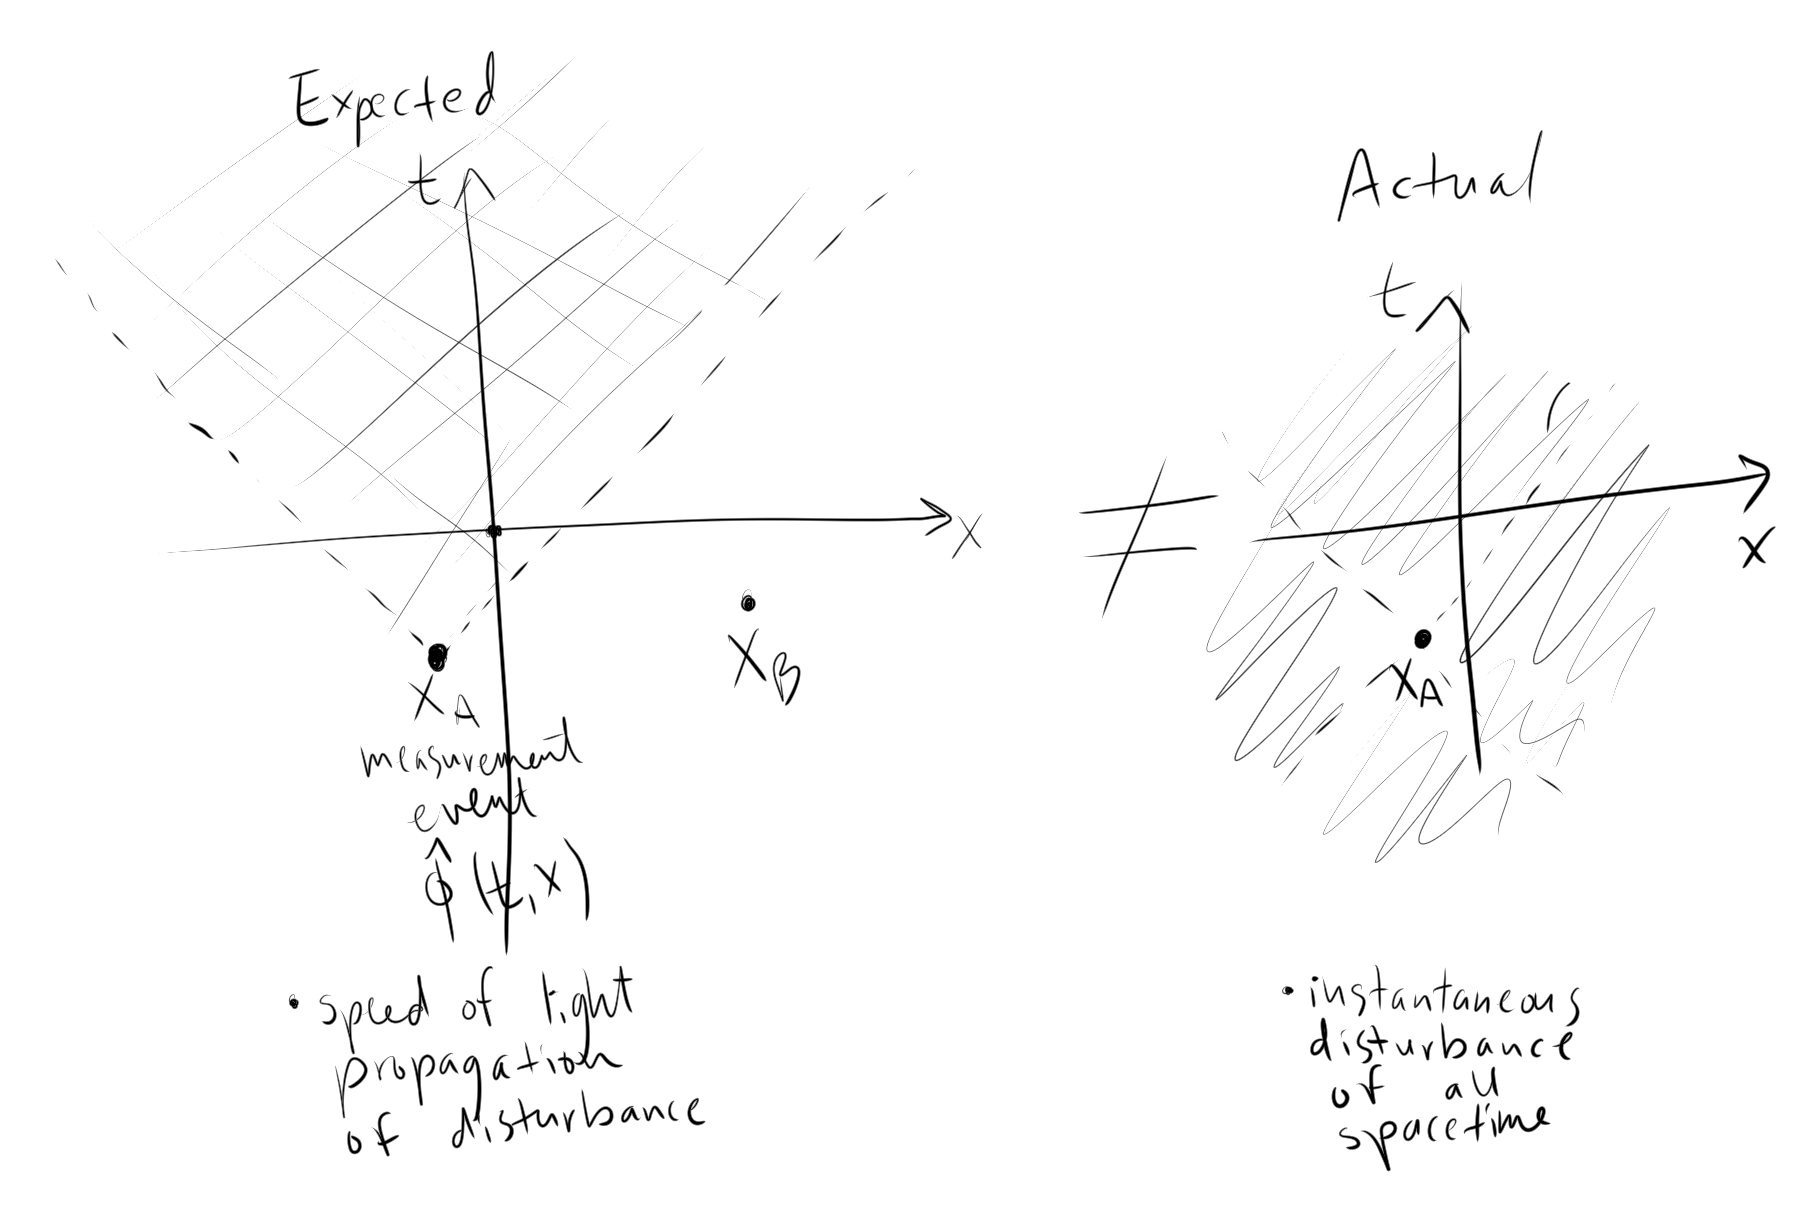
\includegraphics[scale=0.3]{images/lightcone.png}
	\caption{Sketch of expected propagation of information (at the speed of light) due to measurement event of the field $\hat{\phi}(t,x)$.}
\end{figure}

\noindent The result is that no information may be transmitted via the field across a space-like interval ($(x_A - x_B)^2 < 0$). \\

\noindent Now, we have to agree on which quantities are observable, and a natural guess is to study the correlation function
\begin{equation}
\bra{0} \hat{\phi}(x^0,x) \hat{\phi}(y^0,y) \ket{0}.
\end{equation}

\noindent This is unfortunately wrong, since the correlation function has no operational meaning, and can not be directly measured, since the field operators are not Hermitian, in general. \\

\noindent \textbf{Digression: Interference experiment} \\

\noindent To study correlation functions which can be measured in the lab via experiment, consider the following interference experiment set up with a Klein-Gordon field with auxiliary modes of light used to perform measurements and generate results. \\

\begin{figure}[H]
	\centering
	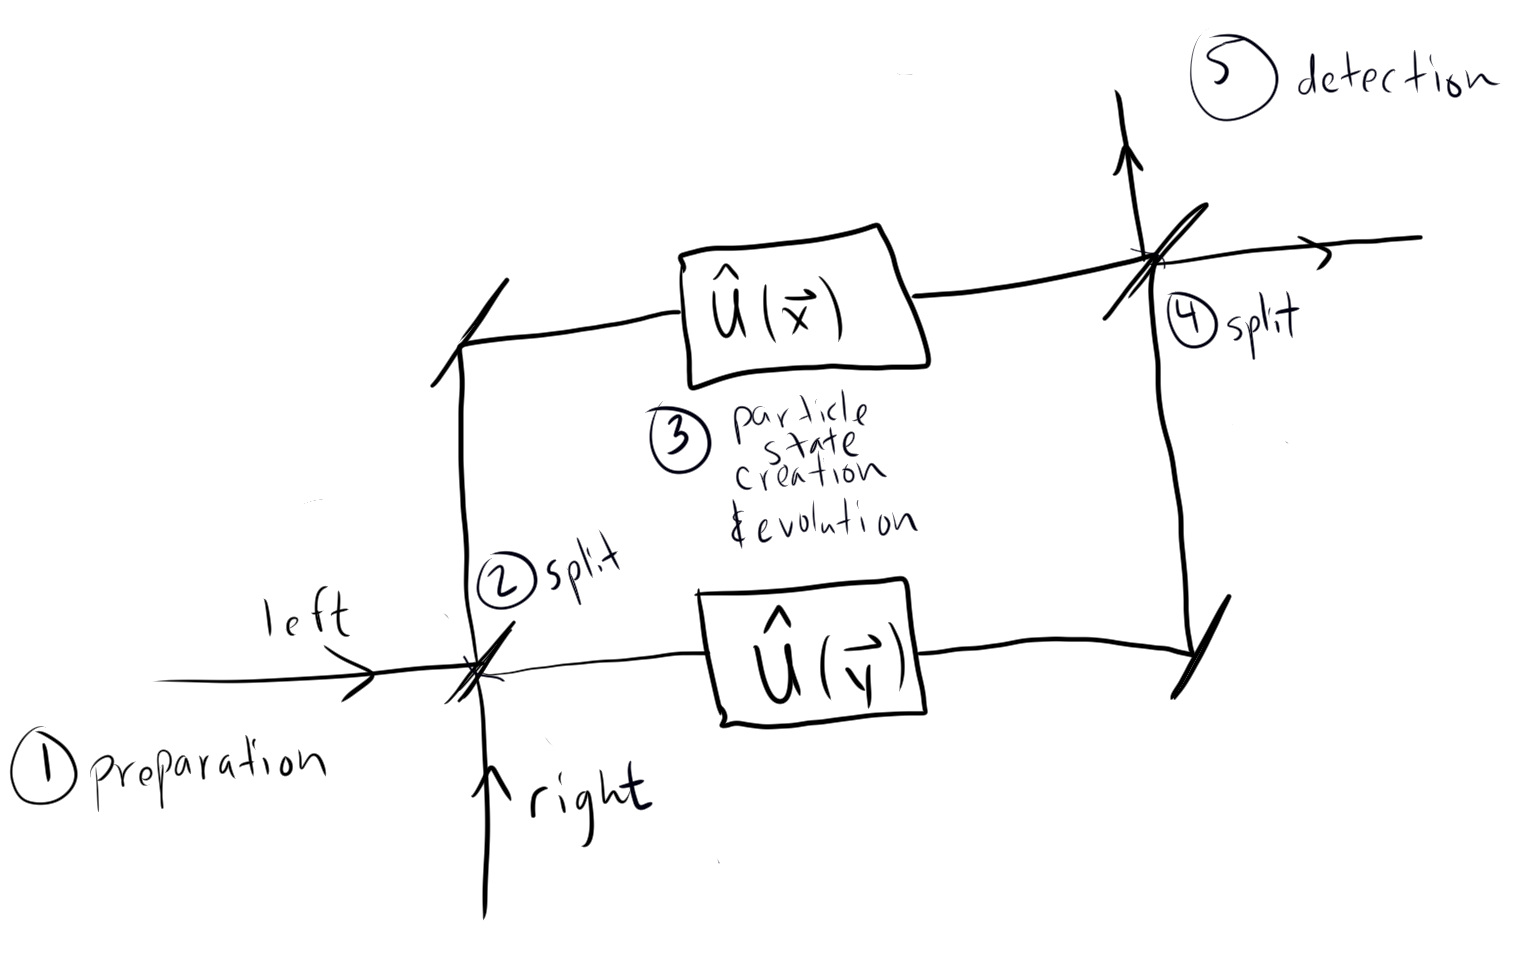
\includegraphics[scale=0.4]{images/interference.png}
	\caption{Schematic of experiment to measure the correlation of two spacetime locations and the Klein-Gordon field under measurement.}
\end{figure}

\begin{enumerate}
\item Prepare the field and auxiliary system (left and right) in the vacuum state
	\begin{equation}
	\ket{0}_{field} \ket{0}_{left} \ket{0}_{right}.
	\end{equation}
\item Apply the Hadamard gate (beam splitter) to the left and right auxiliary states
	\begin{equation}
	\ket{0}_{field} \left( \frac{1}{\sqrt{2}} \left( \ket{0}_{left} \ket{1}_{right} + \ket{1}_{left} \ket{0}_{right} \right) \right).
	\end{equation}
\item Create a particle at $\textbf{x}$ or $\textbf{y}$ via the unitary operator
	\begin{equation}
	\hat{U}(\textbf{x}) \otimes \ket{1}\bra{1}_{left} \otimes \mathbb{I}_{right} + \hat{U}(\textbf{y}) \otimes \mathbb{I}_{left} \ket{1}\bra{1}_{right}
	\end{equation}
	Applied to the state in \textbf{Step 2}, which evolves to the state (dropping "left" and "right" labels)
	\begin{equation}
	\frac{1}{\sqrt{2}} \left( \hat{U}(\textbf{y}) \ket{0}_{field} \ket{0 \, 1} + \hat{U}(\textbf{x}) \ket{0}_{field} \ket{1 \, 0} \right)
	\end{equation}
\item Apply a second beam splitter to the auxiliary states to check for interference in the final state
	\begin{equation}
	\frac{1}{2} \left( \hat{U}(\textbf{x}) + \hat{U}(\textbf{y}) \right) \ket{0}_{field} \ket{0 \, 1} + \frac{1}{2} \left( \hat{U}(\textbf{x}) - \hat{U}(\textbf{y}) \right) \ket{0}_{field} \ket{1 \, 0}
	\end{equation}
\item Detect auxiliary states $\ket{0 \, 1}$ and $\ket{1 \, 0}$.  
\end{enumerate}

\noindent The probability of measuring one of the states, $\ket{0 \, 1}$, for example, is 
\begin{align}
\mathcal{P}(\ket{0 \, 1}) &= \frac{1}{4} \bra{0}_{field} \left( \hat{U}^\dagger(\textbf{x}) + \hat{U}^\dagger(\textbf{y}) \right) \left( \hat{U}(\textbf{x}) + \hat{U}(\textbf{y}) \right)  \ket{0}_{field} \\
&= \frac{1}{2} + \frac{1}{2} Re \left[ \bra{0}_{field} \hat{U}^\dagger(\textbf{x}) \hat{U}(\textbf{y}) \ket{0}_{field} \right] \\
&= \frac{1}{2} + \frac{1}{2} Re \left[ \bra{0}_{field} e^{-i \epsilon \hat{\phi}(\textbf{x})} e^{i \epsilon \hat{\phi}(\textbf{y})} \ket{0}_{field} \right] \\
\mathcal{P}(\ket{0 \, 1}) &= \frac{1}{2} + \frac{1}{2} Re \left[ \bra{0}_{field} e^{-i \epsilon \hat{\phi}(\textbf{x})+ i \epsilon \hat{\phi}(\textbf{y}) +\frac{1}{2} \epsilon^2 [ \hat{\phi}(\textbf{x}), \hat{\phi}(\textbf{y}) ] } \ket{0}_{field} \right] \\
\end{align}

\noindent Where the last line is gotten via the Baker-Campbell-Hausdorff relation, since the two fields operators do not necessarily commute, and the interference between the two measurement events is determined by whether the commutator is zero or nonzero, which is calculated \\
\begin{align}
[ \hat{\phi}(\textbf{x}), \hat{\phi}(\textbf{y}) ] &= \int \frac{d^3 p}{(2\pi)^3} \int \frac{d^3 q}{(2\pi)^3} \frac{1}{\sqrt{4 \omega_p \omega_q}} \left( [\hat{a}_p, \hat{a}_q^\dagger ] e^{-i \textbf{p} \cdot \textbf{x} + i \textbf{q} \cdot \textbf{y}} + [\hat{a}_p^\dagger, \hat{a}_q ] e^{i \textbf{p} \cdot \textbf{x} - i \textbf{q} \cdot \textbf{y}} \right) \\
&= \int \frac{d^3 p}{(2\pi)^3} \frac{1}{\sqrt{2 \omega_p}} \left( e^{-i \textbf{p} \cdot (\textbf{x}-\textbf{y})} - e^{i \textbf{p} \cdot (\textbf{x}-\textbf{y})} \right) \cdot \mathbb{I} \\
[ \hat{\phi}(\textbf{x}), \hat{\phi}(\textbf{y}) ] &= \Delta (\textbf{x} - \textbf{y}) \cdot \mathbb{I}
\end{align}

\noindent Where the commutation relation $[\hat{a}_p, \hat{a}_q^\dagger] = (2\pi)^3 \delta^{(3)} (p-q) \cdot \mathbb{I}$ is used, and the quantity $\Delta (\textbf{x} - \textbf{y})$, the \textbf{correlation function}, which is Lorentz invariant, must be zero when $\textbf{x}$ and $\textbf{y}$ are space-like separated, such that $(\textbf{x} - \textbf{y})^2 < 0$. \\

\noindent Consider the space-like separation, $(\textbf{x} - \textbf{y})^2 < 0$, and enter a reference frame where $\textbf{x} - \textbf{y} = (0, x-y)$, and the correlation function $\Delta (\textbf{x} - \textbf{y})$ becomes zero!
\begin{align}
\Delta (\textbf{x} - \textbf{y}) &= \frac{1}{2} \int \frac{d^3 p}{(2\pi)^3} \frac{1}{\sqrt{|p|^2+m^2}} \left( e^{i p \cdot (x-y)} - e^{-ip \cdot (x-y)} \right) \\
&= \frac{1}{2} \int \frac{d^3 p}{(2\pi)^3} \frac{1}{\sqrt{|p|^2+m^2}} \left( e^{i p \cdot (x-y)} - e^{ip \cdot (x-y)} \right) \\
\Delta (\textbf{x} - \textbf{y}) &= 0
\end{align}

\noindent Where the second line is gotten by applying the Lorentz transformation $(x-y) \rightarrow -(x-y)$, which is allowed for in a space-like interval. \\

\begin{figure}[H]
	\centering
	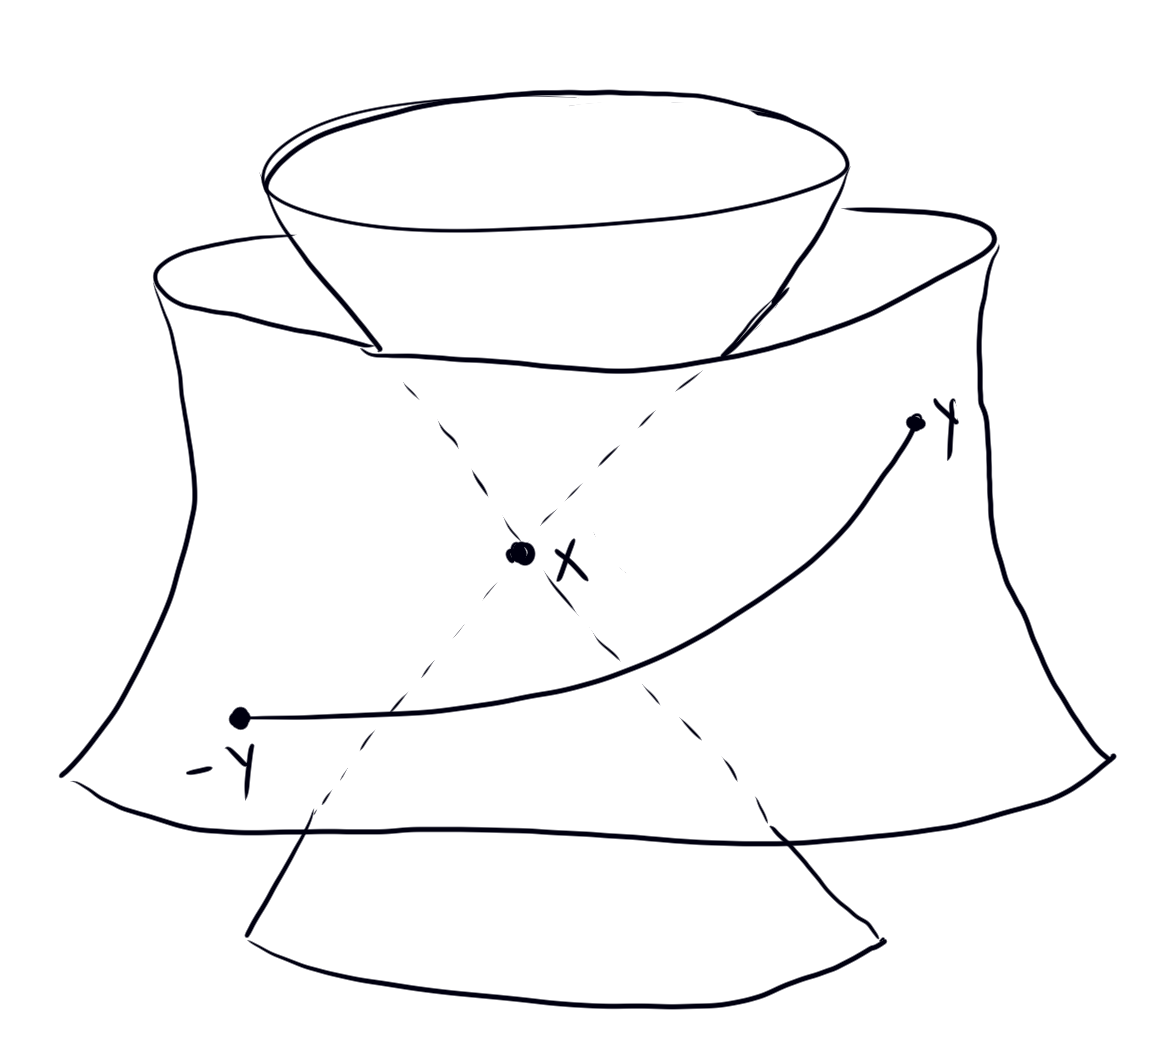
\includegraphics[scale=0.3]{images/inversion.png}
	\caption{Sketch of spatial inversion of spacetime location $\textbf{y}$.}
\end{figure}

\noindent Therefore, information does not travel faster than the speed of light, and the field operators respect causality when they are space-like separated! Note that this does not yet prove that the entire theory is causal. \\

\noindent As a side note, consider the case where the two field measurements are time-like separated, such that $(\textbf{x} - \textbf{y})^2 > 0$, and enter a reference frame where $\textbf{x} - \textbf{y} = (t, 0, 0, 0)$. In this reference frame of time-like separation, the correlation function can \textbf{not} be zero
\begin{align}
\Delta (\textbf{x} - \textbf{y}) &= \int \frac{d^3 p}{(2\pi)^3} \frac{1}{\sqrt{2 \omega_p}} \left( e^{-i\omega_p t} - e^{i\omega_p t} \right) \\
&= \frac{1}{4\pi^2} \int_m^{\infty} dE \, \sqrt{E^2 + m^2} e^{-iEt} \\
\Delta (\textbf{x} - \textbf{y}) &\sim e^{-imt} - e^{imt} \ne 0 .
\end{align}

\noindent Return to consider the (non-physical) two-point correlation function in a space-like interval
\begin{align}
D(\textbf{x}-\textbf{y}) &= \bra{0} \hat{\phi}(\textbf{x}) \hat{\phi}(\textbf{y}) \ket{0} \\
&= \int \frac{d^3 p}{(2\pi)^3} \frac{1}{2 \omega_p} e^{-i \textbf{p} \cdot (\textbf{x}-\textbf{y})} \\
&= \frac{1}{2} \int \frac{d^3 p}{(2\pi)^3} \frac{1}{\sqrt{|p|^2 + m^2}} e^{i p \cdot( x-y)} \\
&= \frac{m}{4\pi^2} \frac{1}{|x-y|} K_1(m|x-y|) \\
D(\textbf{x}-\textbf{y}) &\sim e^{-m|x-y|} \ne 0
\end{align}

\noindent Where $K_1(x)$ denotes the Hankel function. \\

\noindent So, when $\textbf{x}$ and $\textbf{y}$ are space-like separated, this correlation function can not be zero, and can therefore not carry any information, as it would have to travel faster than the speed of light. \\

\noindent An important application of the correlation function is the \textbf{Feynman propagator}, which is used later in perturbative expansions for describing interactions.
\begin{align}
    \Delta_F (\textbf{x} - \textbf{y}) &=
    \begin{cases}
      D(\textbf{x} - \textbf{y}), & x^0 > y^0 \\
      D(\textbf{y} - \textbf{x}), & x^0 < y^0
    \end{cases} \\
\Delta_F (\textbf{x} - \textbf{y}) &= \bra{0} \mathcal{T} [ \hat{\phi}(\textbf{x}) \hat{\phi}(\textbf{y}) ] \ket{0}
\end{align}

\noindent Where $\mathcal{T[\,]}$ is called the \textbf{time-ordering operator}
\begin{equation}
\mathcal{T} [ \hat{\phi}(\textbf{x}) \hat{\phi}(\textbf{y}) ] =
    \begin{cases}
      \hat{\phi}(\textbf{x}) \hat{\phi}(\textbf{y}), & x^0 > y^0 \\
      \hat{\phi}(\textbf{y}) \hat{\phi}(\textbf{x}), & x^0 < y^0
    \end{cases}
\end{equation}

\noindent Another important definition of the Feynman propagator is in terms of complex variables and contour integrals. \\

\noindent \textbf{Lemma:} 
\begin{align}
\Delta_F (\textbf{x} - \textbf{y}) &= \int \frac{d^4 p}{(2\pi)^4} \frac{i e^{-i \textbf{p} \cdot (\textbf{x}-\textbf{y})}}{|\textbf{p}|^2 - m^2 +i \epsilon} \\
&= \int \frac{d^3 p}{(2\pi)^3} \int_C \frac{d p^0}{2\pi} \frac{i e^{-i \textbf{p} \cdot (\textbf{x}-\textbf{y})}}{|\textbf{p}|^2 - m^2 +i \epsilon}
\end{align}

\noindent Where the integrand of the contour integral over the complex variable $p^0$ has two poles at $\pm i\epsilon$, and the contour is taken along the real $p^0$ axis, and closed in the upper or lower half-plane, depending on the value of $p^0$. \\

\begin{figure}[H]
	\centering
	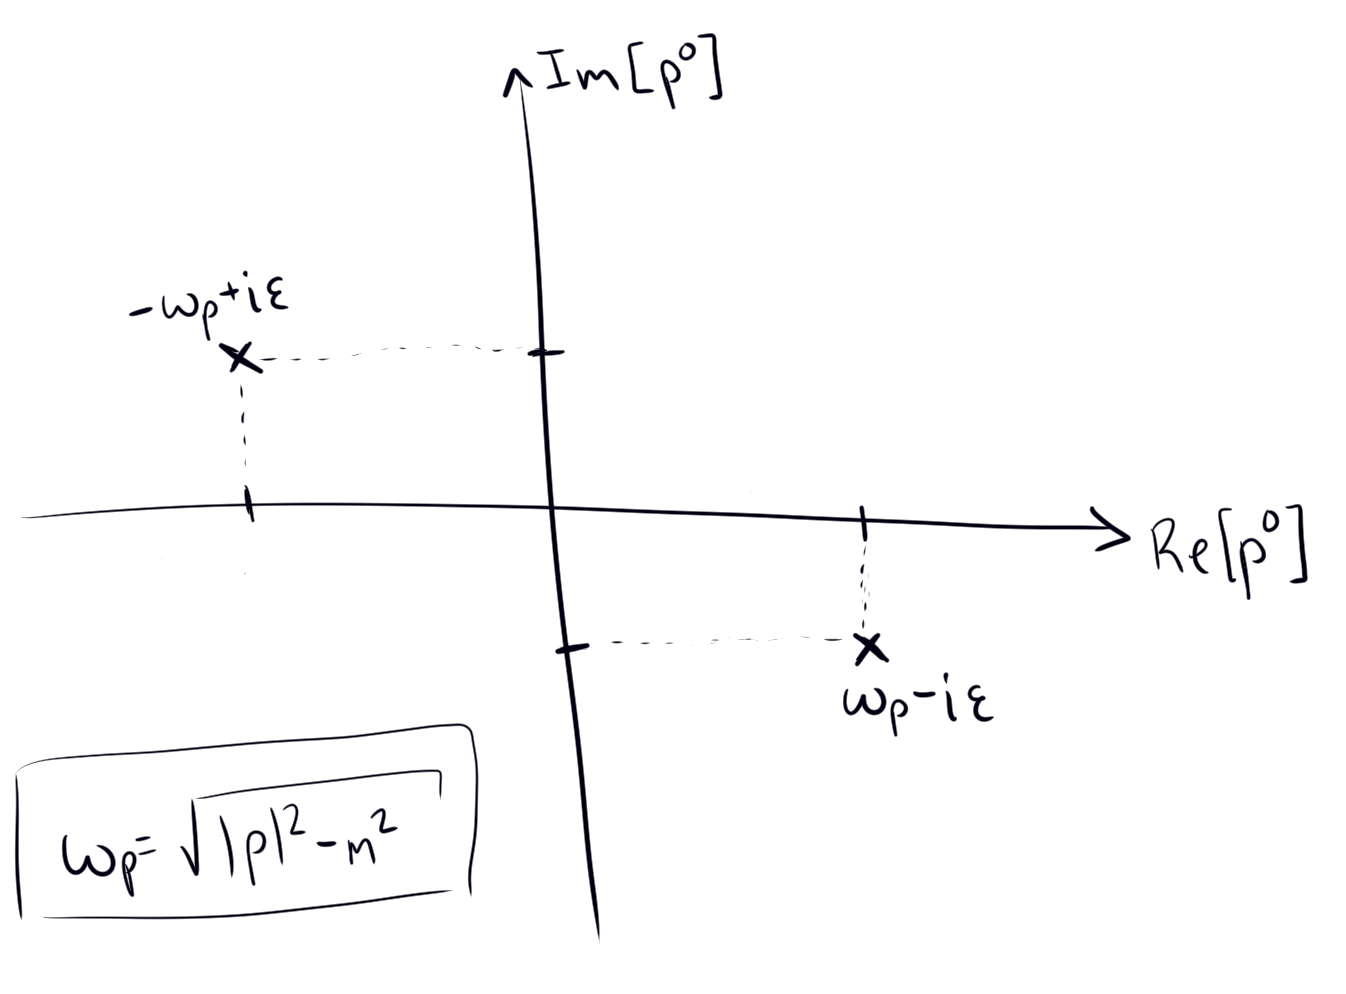
\includegraphics[scale=0.5]{images/poles.png}
	\caption{Poles of the Feynman propagator, where the contour may be taken in the upper half-plane for $t<0$, and in the lower half-plane for $t>0$, where $t=x^0-y_0$.}
\end{figure}

\noindent Lastly, an observation that the Feynman propagator, which is related thus far to the two-point correlation function, is also a Green's function (inverse of a differential operator) for the Klein-Gordon partial differential equation
\begin{align}
(\partial_0^2 - \nabla^2 + m^2) \Delta_F(\textbf{x} - \textbf{y}) &= -i \delta^{(4)} (\textbf{x} - \textbf{y}) \\
\sim \hat{\mathbb{L}} \cdot \hat{\mathbb{L}}^{-1} &= \mathbb{I}
\end{align}

\noindent Where the left-hand side is the product of a linear differential operator, the Klein-Gordon operator, and its inverse, the Feynman propagator, and the right-hand side of the equation is, in essence, the identity.

\clearpage

\section{Lecture 7: Representing Symmetries in QFT}
\label{sec:lec7}

\noindent Here we finish study of the quantum Klein-Gordon field by working out how the Lorentz group is unitarily represented on the space of states on the Klein-Gordon field. Recall that for a relativistic quantum field theory, we must have a (projective) unitary representation of the Poincar\'e group $U(\Lambda, a)$ on a Hilbert space $\mathcal{H}$. Thus far, we have constructed the Hilbert space, with respect to some norm $|| \cdot ||$, as the space of states gotten by applying creation operators to the vacuum state

\begin{equation}
\mathcal{H} = span \{ \hat{a}_{\textbf{p}_1}^\dagger \hat{a}_{\textbf{p}_2}^\dagger \dots \hat{a}_{\textbf{p}_n}^\dagger \ket{\Omega} \} ^{||\cdot||}
\end{equation}

\subsection*{Digression: Continuous Groups of Symmetries}

\noindent The central idea of a group with a continuous manifold structure (e.g., Lie groups) is to study symmetries close to, localized to, the identity and then exponentiate to larger, more global, elements. Important continuous operations on this manifold $\mathcal{M}$ include (closed) composition and inverse. \\

\begin{figure}[H]
	\centering
	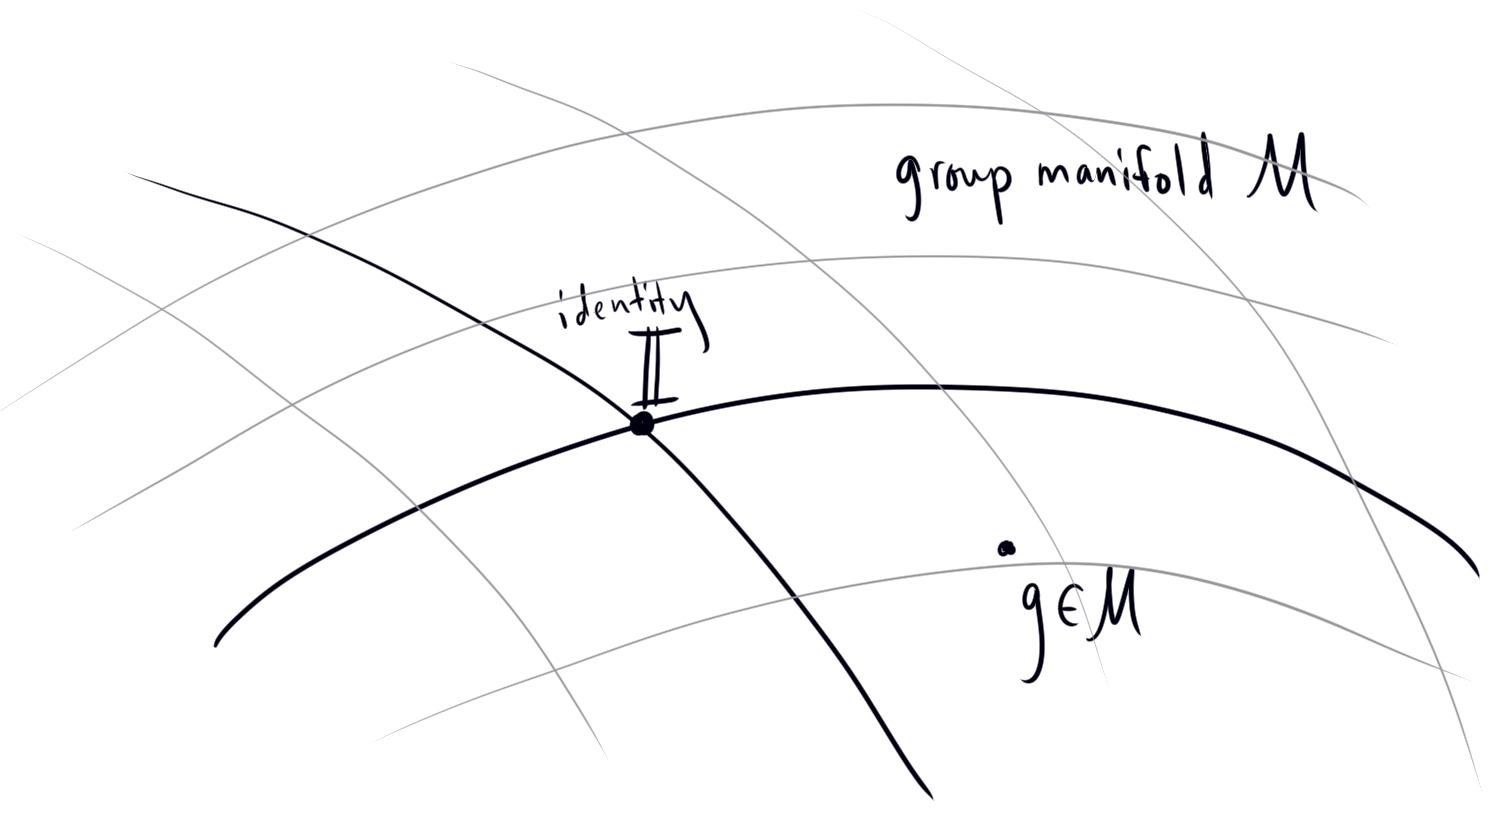
\includegraphics[scale=0.3]{images/groupmanifold.png}
	\caption{Sketch of a group manifold with identity $\mathbb{I}$ and an element of the manifold $g$.}
\end{figure}

\begin{align}
\text{Closure:} \,\,\,\,\, \mathcal{M} \times \mathcal{M} &\rightarrow \mathcal{M} \\
g \times h &\rightarrow g \cdot h \\
\text{Inverse:} \,\,\,\,\,\,\,\,\,\,\,\,\,\,\,\,\,\,\,\, \mathcal{M} &\rightarrow \mathcal{M} \\
g &\rightarrow g^{-1}
\end{align}

\noindent The Poincar\'e group is an example of a continuous Lie group, and to understand its structure, consider elements $g \in \mathcal{M}$ infinitesimally close to the identity $\mathbb{I}$, such that $g - \mathbb{I} \sim \mathcal{O}(\epsilon)$. These infinitesimal elements are elements of the tangent space $T_{\mathbb{I}} \, \mathcal{M}$, which is a linear space and is called a \textit{Lie algebra}. The basis vectors of $T_{\mathbb{I}} \, \mathcal{M}$ are written as $x^j$, $j=1,2,\dots,dim(\mathcal{M})$.

\subsection*{Examples of Tangent Spaces}

\begin{enumerate}
\item $1 \times 1$ unitary matrices $U(1) = \{ \phi \in \mathbb{C} : |\phi|^2 = 1 \}$
\subitem $\rightarrow T_1 \, U(1) = \{ z: (1+\epsilon z)^* (1+\epsilon z) = 1$ to order $\epsilon$,  s.t. $Re[z]=0) \}$

\item $3 \times 3$ Euclidean rotation matrices $O(3) = \{ O \in \mathcal{M}_3(\mathbb{R}) : O^T O = \mathbb{I} \}$
\subitem $\rightarrow T_{\mathbb{I}} \, O(3) = \{ X : (\mathbb{I} + \epsilon X)^T (\mathbb{I} + \epsilon X) = \mathbb{I}$ to order $\epsilon$, s.t. $X + X^T = 0 \}$
\subitem - Note that including inversions promotes $O(3)$ to $SO(3)$.
\subitem - Basis of $O(3) = \\ \{ X = \sum_{j=1}^3 X_j J^j : J^1 = \left(\begin{smallmatrix} 0&1&0 \\ -1&0&0 \\ 0&0&0 \end{smallmatrix}\right), J^2 = \left(\begin{smallmatrix} 0&0&1 \\ 0&0&0 \\ -1&0&0 \end{smallmatrix}\right), J^3 = \left(\begin{smallmatrix} 0&0&0 \\ 0&0&1 \\ 0&-1&0 \end{smallmatrix}\right) \}$

\item $4 \times 4$ Lorentz transformation matrices $G = \{ \Lambda : \eta_{\mu\nu} \Lambda^\mu_{\,\,\,\rho} \Lambda^\nu_{\,\,\,\sigma} = \eta_{\rho\sigma} \}$ 
\subitem \begin{align*}
\rightarrow T_{\mathbb{I}} \, G &= \{ \omega : \eta_{\mu\nu} (\mathbb{I} + \epsilon \omega)^\mu_{\,\,\,\rho} (\mathbb{I} + \epsilon \omega)^\nu_{\,\,\,\sigma} = \eta_{\rho\sigma} \} \\
&= \{ \omega : \text{antisymmetric, s.t. } \omega^{\mu\nu} = -\omega^{\nu\mu} \} \\
&\,\,\,\,\,\,\, {\scriptsize \text{Note the "upstairs" covariant indices on }} \omega \\
&\,\,\,\,\,\,\, {\scriptsize \text{Using "downstairs" contravariant indices}} \\ 
&\,\,\,\,\,\,\, {\scriptsize \text{requires multiplication by the metric } \eta_{\mu\nu} \text{ as above.}} \\
&= \{ \omega : \text{change of basis to } \omega = \sum_{j=1}^6 \frac{1}{2} \Omega_j J^j \} \\
&\,\,\,\,\,\,\, {\scriptsize \text{Change indices via the bijection } j \rightarrow (\rho \, \sigma), \text{with } 0<\rho<\sigma\le 3 } \\
&\,\,\,\,\,\,\,\,\,\,\,\,\,\,\,\,\,\, 1 \rightarrow (0 \, 1); \, 2 \rightarrow (0 \, 2); \, 3 \rightarrow (0 \, 3) \\
&\,\,\,\,\,\,\,\,\,\,\,\,\,\,\,\,\,\, 4 \rightarrow (1 \, 2); \, 5 \rightarrow (1 \, 3); \, 6 \rightarrow (2 \, 3) \\
&= \tag{\textbf{Exercise}} \{ \omega : \text{with index bijection } \omega = \sum_{(\rho\sigma)} \frac{1}{2} \Omega_{(\rho\sigma)}  J^{(\rho\sigma)}  \} \\
&\,\,\,\,\,\,\,\,\,\,\, {\scriptsize \text{This bijection allows the basis to be expressed }}  \\
&\,\,\,\,\,\,\,\,\,\,\, {\scriptsize \text{by the formula } [J^{(\rho\sigma)}]^\mu_{\,\,\nu} = \eta^{\rho\sigma} \delta^{\sigma}_{\,\,\nu} - \eta^{\sigma\mu} \delta^{\rho}_{\,\,\nu}} \\
\end{align*}
\end{enumerate}

\noindent Understanding the structure of a linear space infinitesimally close to the identity yields information about the whole Lie group and the global structure of the manifold. Also note that multiplication on this linear space is a continuous map that strongly determines the group structure on the manifold. \\

\noindent To demonstrate how a Lie algebra on the (linear) tangent space produces a Lie group, and vice versa, consider the element of the tangent space of a manifold $X \in T_{\mathbb{I}} \, \mathcal{M}$, such that $\mathbb{I} + s X \sim e^{\epsilon X} \in \mathcal{M}$, to order $\epsilon$. \\

\noindent Define the function $g(s) = \lim_{n\to\infty} (\mathbb{I} + \frac{s}{n} X)^n = e^{s X} \in \mathcal{M}$. Therefore, every element of the Lie algebra (tangent space to the identity) determines an element of the Lie group (manifold). To go the other way, and determine the Lie algebra from the Lie group, apply the logarithm map.\\

\begin{figure}[H]
	\centering
	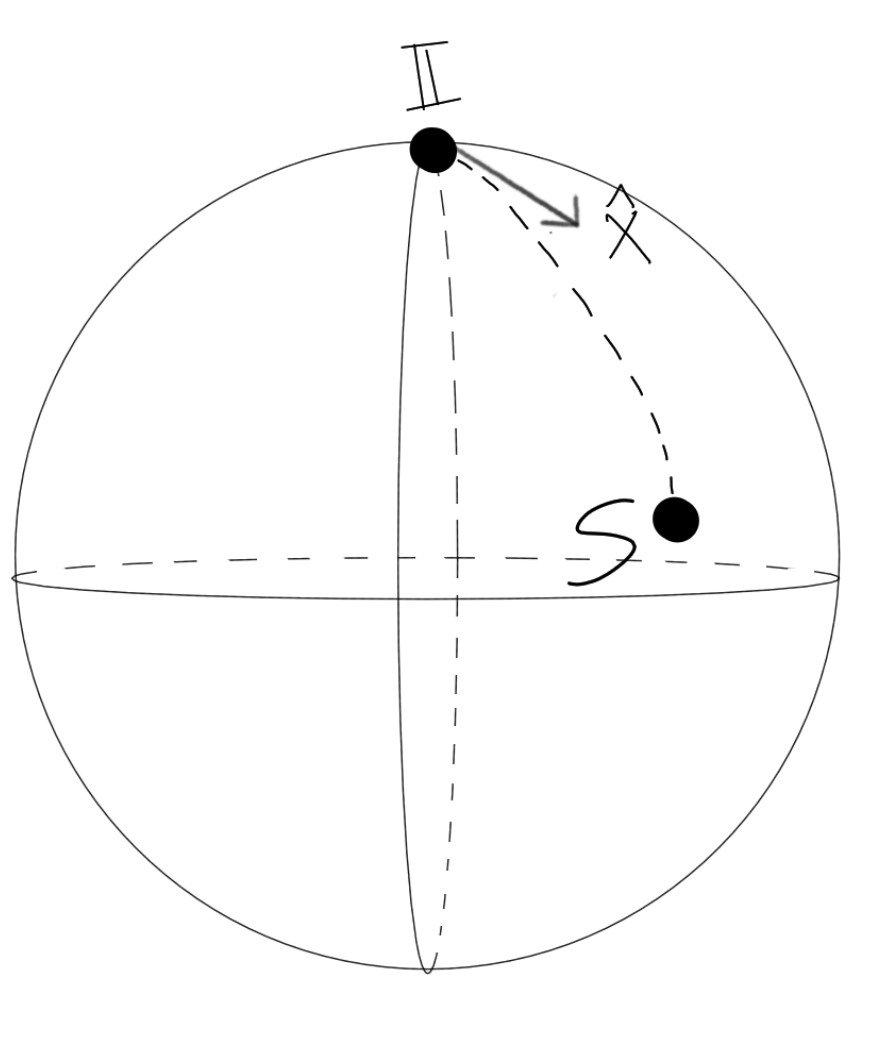
\includegraphics[scale=0.4]{images/exponentiation.png}
	\caption{Figure of exponentiation map on Lie group (e.g., $O(3)$) manifold. Translation from identity a distance $s$ along the $X$ direction. Resulting position on manifold is called the exponential of $s X$.}
\end{figure}

\subsection*{Algebraic structure on tangent space}

\noindent The algebraic structure on the tangent space is defined by the \textit{group commutator} on the manifold, which is also a group. 
\begin{align}
[\, , \,] : \mathcal{M} \times \mathcal{M} &\rightarrow \mathcal{M} \\
(g, h) &\rightarrow [g, h] = ghg^{-1}h^{-1}, \, \forall \, g, h \in \mathcal{M}
\end{align}

\noindent The group commutator also pushes forward to a mapping of the tangent space
\begin{equation}
[\, , \,] : T_{\mathbb{I}} \, \mathcal{M} \times T_{\mathbb{I}} \, \mathcal{M} \rightarrow T_{\mathbb{I}} \, \mathcal{M}
\end{equation}

\noindent Consider the following group commutator which is an element of the manifold
\begin{align}
[\mathbb{I} + \epsilon X, \mathbb{I} + \delta Y] &= (\mathbb{I} + \epsilon X) (\mathbb{I} + \delta Y) (\mathbb{I} - \epsilon X) (\mathbb{I} - \delta Y) \\
&= \mathbb{I} + \epsilon \delta (XY - YX) + \mathcal{O}(\epsilon^2) + \mathcal{O}(\delta^2) + \dots \\
&\sim \mathbb{I} + \epsilon \delta [X, Y]
\end{align}

\noindent Where $\epsilon$ and $\delta$ are small, independent parameters, and the Lie algebra commutator $[X, Y]$ is, therefore, an element of the tangent space of the manifold, such that $[X,Y] \in T_{\mathbb{I}} \, \mathcal{M}$. \\

\subsection*{Examples of Lie algebra commutators}

\begin{enumerate}
\item $U(1)$: trivial
\item $O(3)$: $[J^j, J^k] = -\epsilon^{jk}_{\,\,\, l} J^l$ 
\item Lorentz group: $[J^{\rho\sigma}, J^{\tau\nu}] = \eta^{\sigma\tau}J^{\rho\nu} - \eta^{\rho\tau}J^{\sigma\nu} + \eta^{\rho\nu}J^{\sigma\tau} - \eta^{\sigma\nu}J^{\rho\tau}$

\subitem E.g., \[ [J^{01}]^\mu_{\,\,\, \nu} = 
\left( 
\begin{array}{@{}c|c@{}}
\begin{matrix} 0 & 1 \\ 1 & 0 \end{matrix} & \bigzero \\
\hline
\bigzero & \begin{matrix} 0 & 0 \\ 0 & 0 \end{matrix} 
\end{array} \right), \,\, [J^{12}]^\mu_{\,\,\, \nu} = 
\left( 
\begin{array}{@{}c|c@{}}
\bigzero & \begin{matrix} 0 & 0 \\ -1 & 0 \end{matrix} \\
\hline
\begin{matrix} 0 & 1 \\ 0 & 0 \end{matrix} & \bigzero
\end{array} \right) \]

\subitem \[ [J^{01}, J^{12}] = -J^{13} =  
\left( 
\begin{array}{@{}c|c@{}}
\bigzero & \begin{matrix} 0 & 0 \\ 0 & -1 \end{matrix} \\
\hline
\begin{matrix} 0 & 0 \\ 0 & 1 \end{matrix} & \bigzero
\end{array} \right) \]

\subitem Special names for this particular Lie group elements in the Lorentz transformation
\subsubitem \textbf{Generators of boosts} (pure boost by exponentiating, s.t. $e^{\frac{1}{2} \epsilon_j K^j}$): 
\subsubitem $J^{0j} = K^j$
\subsubitem \textbf{Generators of rotations} (elements of $O(3) \subset$ Lorentz group): 
\subsubitem $J^{12} = J^1, \, J^{13} = J^2, \, J^{23} = J^3$
\end{enumerate}

\subsection*{Representations of Lie groups}

Consider a representation $\pi$ of the Lie algebra $T_\mathbb{I}\,\mathcal{M}$ which is a linear map from the tangent space to the Hilbert space of bounded linear operators, such that the Lie bracket property is preserved, such that $[\pi(X), \pi(Y)] = \pi([X,Y])$
\begin{equation}
\pi : T_\mathbb{I}\,\mathcal{M} \rightarrow \mathcal{B} (\mathcal{H})
\end{equation}

\noindent This representation is exponentiated to a representation of the Lie group manifold $\mathcal{M}$
\begin{equation}
\pi(g = e^{\epsilon X}) = e^{\epsilon \pi(X)}
\end{equation}

\noindent This shows that one can either try to find matrices that obey the Lie group law, or, more easily, focus on the Lie algebra (linear space) and find matrices that obey the Lie bracket property; Lie group representations are often not worked with directly, but the elements of the Lie algebra can just be exponentiated to obtain the representation of the Lie group. \\

\noindent To implement a general Lorentz transformation on the Hilbert space of states allowed in the Klein-Gordon field, Noether's theorem, as well as the \textit{inverse Noether's theorem}, is employed. Noether's theorem allows conserved currents to be derived from symmetry transformations. Information in thrown out when integrating the currents over space $\int d^3 x$ to get the conserved charge, but the time-like component is left alone, and information about the structure of the symmetry transformation is conserved, which can be gotten back by the inverse Noether's theorem. \\

\noindent \textbf{Recap of Noether's theorem:} For each symmetry of a field, with respect to a coordinate transformation $x \rightarrow \exp^{\epsilon J ^{\rho\sigma}}$, there exists a conserved current per $J^{\rho\sigma}$. For example, the group of Lorentz transformations is described by six independent parameters, the generators of the transformation, associated with six conserved currents. The conserved currents from the symmetries of the Lorentz transformation have the form
\begin{equation}
\mathcal{J}^{(\rho\sigma)} = \textbf{x}^\rho T^{\mu\sigma} - \textbf{x}^\sigma T^{\mu\rho}
\end{equation}

\noindent Where $\textbf{x}^\mu$ are 4-vector spacetime coordinates, and $T^{\mu\nu}$ are elements of the energy-momentum tensor. The conserved charges are then gotten by integrating over space
\begin{equation}
Q^{(\rho\sigma)} = \int d^3 x \, \mathcal{J}^{(\rho\sigma)} = \int d^3x \,  (\textbf{x}^\rho T^{0\sigma} - \textbf{x}^\sigma T^{0\rho})
\end{equation}
\\
\textit{"Noether's theorem is really just a fancy telescoping series in disguise."} \\

\noindent The arguably more profound statement regarding conserved charges and symmetries is the inverse Noether's theorem. \\

\noindent \textbf{Inverse Noether's theorem:} Conserved charges are the generators, represent the Lie algebra, of the symmetry transformations from which they came, and generate canonical transformations, or representations of the symmetries, on phase space. Classically, 
\begin{equation}
\{Q^{(\rho\sigma)}, Q^{(\tau\nu)}\}_{PB} = \eta^{\sigma\tau}Q^{\rho\nu} - \eta^{\rho\tau}Q^{\sigma\nu} + \eta^{\rho\nu}Q^{\sigma\tau} - \eta^{\sigma\nu}Q^{\rho\tau}
\end{equation}

\noindent Propose that we "just put hats on" the conserved charges, and check that they obey the Lie algebra of the Lorentz group. It turns out that this works for free theories, and we have, at least, one representation of the Lie algebra of the Lorentz group in the context of one, the Klein-Gordon, quantum field.
\begin{equation}
\hat{Q}^{\mu\nu} = \int d^3 x (x^\mu \hat{T}^{0\nu} - x^\nu \hat{T}^{0\mu})
\end{equation}

\noindent Consider the $0j^{th}$ conserved charge, using the specialized notation, and check that $\hat{Q}^{0j} = \hat{K}^j$ does indeed generate boosts and is time independent.
\begin{align}
\hat{Q}^{0j} = \hat{K}^j &= \int d^3 x \, (x^j \hat{T}^{00} - x^0 \hat{T}^{0j}) \\
\hat{K}^j &= -t \, \hat{P}^j + \int d^3 x \, x^j \hat{\mathscr{H}}(t,x) \\
\frac{d \hat{K}^j }{dt} &= -\hat{P}^j + i [\hat{H}, \int d^3 x \, x^j \hat{\mathscr{H}}(t,x) ] \\
0 &= \hat{P}^j + i[\hat{H}, \hat{K}^j] \\
[\hat{H}, \hat{K}^j] &= -i \hat{P}^j .
\end{align}

\noindent Where $\hat{P}^j$ is the total field momentum, and $\hat{\mathscr{H}}$ is the Hamiltonian density, which does not commute with the Hamiltonian $\hat{H}$. The third line cancels the time dependence of the two right-hand side terms. This shows that an infinitesimal shift in time and an infinitesimal boost is equal to an infinitesimal shift in space. \\

\noindent Similarly for the generators of rotation, which are manifestly time independent, it must be checked that they obey the correct Lie algebra. 
\begin{equation}
\hat{J}^{jk} = \int d^3 x \, \hat{\pi}(x)(x^j \partial_k - x^k \partial_j) \hat{\phi}(x)
\end{equation}

\noindent To perform a Lorentz transformation on the Hilbert state space, a unitary operator is created by putting some parameters $\Omega$ in front of the generators of rotation and exponentiating
\begin{equation}
\hat{U}(\Lambda) = e^{-\frac{1}{2} \Omega_{\rho\sigma} \hat{J}^{\rho\sigma}}
\end{equation}

\noindent There are 9 commutation relations, that must be checked (\textbf{Exercises}), that yield the full Lie algebra of the Poincar\'e group.
\begin{align}
[\hat{J}^j, \hat{J}^k] &= -i \epsilon^{jk}_{\,\,\,\,l} \hat{J}^l \\
[\hat{J}^j, \hat{K}^k] &= -i \epsilon^{jk}_{\,\,\,\,l} \hat{K}^l \\
[\hat{K}^j, \hat{K}^k] &= i \epsilon^{jk}_{\,\,\,\,l} \hat{J}^l \\
[\hat{J}^j, \hat{P}^k] &= -i \epsilon^{jk}_{\,\,\,\,l} \hat{P}^l \\
[\hat{K}^j, \hat{P}^k] &= i \delta^{jk} \hat{H} \\
[\hat{K}^j, \hat{H}] &= i \hat{P}^j \\
[\hat{J}^j, \hat{H}] &=  [\hat{P}^j, \hat{H}] = [\hat{P}^j, \hat{P}^k] = 0
\end{align}

\noindent This now demonstrates how the Klein-Gordon field gives a full (Lie algebra) representation of the Poincar\'e group, and  proves that to perform a Poincar\'e transformation on a state of Klein-Gordon particles, one simply applies a unitary transformation via exponentiation of the above operators, which are the generators of transformations.

\clearpage

\section{Lecture 8: Interactions in QFT}
\label{sec:lec8}

\noindent Thus far, we have studied the Klein-Gordon quantum field, which evolves with time in the Heisenberg picture via the Klein Hamiltonian $H_{KG}$, the generator of time translations
\begin{equation}
\hat{\phi}(t,x) = e^{i\hat{H}_{KG}t} \hat{\phi}(0,x) e^{-i\hat{H}_{KG}t}.
\end{equation}

\noindent We have obtained a full unitary representation of the Poincar\'e group for the Klein-Gordon field by constucting a space of states in terms of the field position operator $\hat{\phi}$ and the field momentum operator $\hat{\pi}$ via the generator of time translation $\hat{H}$, the generators of spatial translation $\hat{P}^j$, and the conserved charges $\hat{Q}^{\mu\nu}$. This is a \textit{free theory}, where the dynamics of two or more spacetime events evolve completely independently of each other with no interactions between particles and field, and is relatively easy to solve. \\

\noindent To attempt to account for interactions, construct a Hilbert space spanned by states of the form $\{  \hat{a}_p^\dagger \hat{a}_q^\dagger \ket{0} \}$, and add a (spatially localized) momentum distribution
\begin{equation}
\ket{\Phi_2} = \int \frac{d^3 p d^3 q}{(2\pi)^6} \, \phi_x(p) \phi_y(q) \cdot \hat{a}_p^\dagger \hat{a}_q^\dagger \ket{0}
\end{equation}

\noindent This states evolves according to the Hamiltonian
\begin{align}
\ket{\Phi_2(t)} &= e^{-i\hat{H}_{KG}t} \ket{\Phi_2} \\
&= \int \frac{d^3 p d^3 q}{(2\pi)^6} \, \phi_x(p) \phi_y(q) e^{-i\hat{H}_{KG}t} \hat{a}_p^\dagger e^{i\hat{H}_{KG}t} e^{-i\hat{H}_{KG}t}  \hat{a}_q^\dagger e^{i\hat{H}_{KG}t}  \ket{0}
\end{align}

\noindent Where $\hat{H}_{KG}$ is quadratic in the creation operators $\hat{a}_p^\dagger$, meaning that the quantity $e^{-i\hat{H}_{KG}t} \hat{a}_p^\dagger e^{i\hat{H}_{KG}t}$ is linear in the creation operators $\hat{a}_p^\dagger$. Therefore, the particles eveolve independently of each other in this attempted formalism, and there are no interactions, which is unphysical for an interacting theory. \\

\noindent Desired characteristics of the interactions that we are attempting to describe are
\begin{enumerate}
\item Model physical experiments
\item Maintain Lorentz invariance
\item Local interactions
\end{enumerate}

\noindent To fulfill these characteristics, we consider studying models with (classical) Lagrangian densities of the form
\begin{equation}
\mathcal{L} = \frac{1}{2} (\partial_\mu \phi(x))(\partial^\mu \phi(x)) - \frac{1}{2}m^2\phi^2(x) - \sum_{n\ge 3}^\infty \frac{\lambda_n}{n!} \phi^n(x)
\end{equation}

\noindent It will later be shown that Lagrangian densities with $n>4$ are irrelevant to observable physics, and $n=3$ leads to instabilities, and neither case is renormalizable. Therefore, the only relevant \textit{interacting scalar quantum field theory} is the $n=4$ case
\begin{equation}
\mathcal{L} = \frac{1}{2} (\partial_\mu \phi(x))(\partial^\mu \phi(x)) - \frac{1}{2}m^2\phi^2(x) - \frac{\lambda}{4!} \phi^4(x)
\end{equation}

\noindent In a quantum field theory, interactions are handled in several ways
\begin{enumerate}
\item Perturbation theory
	\subitem {\small Expand Hamiltonian in Taylor series in terms of a small parameter} 
	\subitem {\small Leads to a solvable model when this parameter is set to zero}
	\subitem {\small Feynman diagrams systematically handle all interactions in infinite series}
\item Variational methods
	\subitem {\small Approximates the system and minimizes error parameters}
\item Monte Carlo sampling
\item Exact solutions
	\subitem {\small Bethe Ansatz in $(1+1)$ dimensions}
	\subitem {\small Topological QFT in $(2+1)$ dimensions}
	\subitem {\small Supersymmetry in higher dimensions}
	\subitem {\small Large N limit}
\end{enumerate}

\subsection*{Perturbation theory}

\noindent Consider the "small" addition $\hat{H}_{int}$ to the free theory Hamiltonian $\hat{H}_0$ to make the full Hamiltonian $\hat{H}$
\begin{equation}
\hat{H} = \hat{H}_0 + \hat{H}_{int}
\end{equation}

\noindent Technically, we demand that $||\hat{H}_{int}||_\infty << 1$, but it often happens that $||\hat{H}_{int}||_\infty \rightarrow \infty$, where $||\hat{H}_{int}||_\infty$ is the largest eigenvalue that dominates the error estimates. Therefore, we pretend that $||\hat{H}_{int}||_\infty << 1$, and solve the time-dependent Schr\"odinger equation 
\begin{equation}
i\frac{d}{dt}\ket{\psi} = \hat{H}\ket{\psi}
\end{equation}

\subsection*{Interaction picture}

\noindent Enter a new reference frame, the \textbf{interaction picture}, or the \textbf{Heisenberg picture}, where all states and operators from the Schr\"odinger picture, denoted by subscript "$S$", are transformed via
\begin{align}
\ket{\psi_I (t)} &= e^{i\hat{H}_0 t} \ket{\psi_S (t)} \\
\mathcal{O} &= e^{i\hat{H}_0 t} \, \mathcal{O}_S  \, e^{-i\hat{H}_0 t}
\end{align}

\noindent The time evolution on the interaction space of states is then
\begin{align}
i \frac{d}{dt} \ket{\psi_I (t)} &=  i \frac{d}{dt} e^{i\hat{H}_0 t} \ket{\psi_S (t)} \\
&= - \hat{H}_0 e^{i\hat{H}_0 t} \ket{\psi_S (t)}  + i e^{i\hat{H}_0 t} \frac{d}{dt} \ket{\psi_S (t)} \\
&= - \hat{H}_0 e^{i\hat{H}_0 t} \ket{\psi_S (t)} + i e^{i\hat{H}_0 t}(-i\hat{H}\ket{\psi_S (t)}) \\
&= (- \hat{H}_0 e^{i\hat{H}_0 t} + e^{i\hat{H}_0 t} (\hat{H}_0 + \hat{H}_{int})) \ket{\psi_S (t)} \\
&= (\cancel{- \hat{H}_0 e^{i\hat{H}_0 t}} + e^{i\hat{H}_0 t} (\cancel{\hat{H}_0} + \hat{H}_{int})) \cdot e^{-i\hat{H}_0 t} e^{i\hat{H}_0 t} \cdot \ket{\psi_S (t)} \\
i \frac{d}{dt} \ket{\psi_I (t)} &= (\hat{H}_{int})_I (t) \ket{\psi_I (t)} 
\end{align}

\noindent Note: From here we drop the subscript "$I$" on the interaction Hamiltonian 
\begin{equation}
(\hat{H}_{int})_I (t) \rightarrow \hat{H}_{int} (t).
\end{equation}

\noindent The interacting time-dependent solution is
\begin{equation}
\ket{\psi_I (t)}  = \hat{U}(t,t_0) \ket{\psi_I (t_0)}. 
\end{equation}

\noindent Where the operator $\hat{U}(t,t_0)$ is the propagator, and satisfies the equation
\begin{equation}
i \frac{d}{dt} \hat{U}(t,t_0) = \hat{H}_{int} (t) \, \hat{U}(t,t_0)
\end{equation}

\noindent Integrating this equation with respect to $t$ yields a constraint on the propagator
\begin{equation}
\hat{U}(t,t_0) = \mathbb{I} - i \int_{t_0}^t dt' \, \hat{H}_{int} (t') \hat{U}(t',t_0)
\end{equation}

\noindent One way to solve for $\hat{U}(t,t_0)$ is to guess a solution and check if both sides of the constraint equation are equal. \\

\noindent Another approach is through \textit{fixed point iteration}
\begin{enumerate}
\item Make a guess for $\hat{U}(t,t_0)$
\item Evaluate how wrong it is
\item Minimize error by adding and/or modifying terms to guess
\item Repeat, by substituting the old right-hand side into the new right-hand side, until the left-hand side and the right-hand side of the constraint approaach each other
\end{enumerate}

\noindent The repeated substitution of the propagator into the constraint equation produces the \textbf{Dyson series}, where the $n^{th}$ has the form
\begin{equation}
\hat{U}(t,t_0) = (-i)^n \int^t_{t_0} dt' \int^{t'}_{t_0} dt'' \dots \int^{t_{(n-1)}}_{t_0} dt^{(n-1)} \, \hat{H}_{int}(t') \hat{H}_{int}(t'') \dots \hat{H}_{int}(t^{(n-1)})
\end{equation}

\noindent By the triangle inequality and the product inequality, the norm of the $n^{th}$ term has an upper bound
\begin{equation}
|| \int \dots ||_{\infty} \le \frac{(t-t_0)^n}{n!} (|| \hat{H}_{int} ||_\infty^*)^n .
\end{equation}

\noindent And, since $\hat{H}_{int}(t)$ is just unitarily rotated from $\hat{H}_{int}$
\begin{equation}
|| \hat{H}_{int} ||_\infty^* = \sup_{t' \in [t,t_0]} || \hat{H}_{int}(t') ||_\infty = (||\hat{H}_{int}||_\infty)_S .
\end{equation}

\noindent If $||\hat{H}_{int}||_\infty << 1$, the series has a nonzero radius of convergence. \\

\noindent \textbf{Theorem:} $\hat{U}(t,t_0) = \mathcal{T}[ e^{-i \int^t_{t_0} dt' \, \hat{H}_{int}(t')}]$, where $\mathcal{T}[\,]$ is the time-ordering operator. \\

\noindent To prove, expand the right-hand side in a Taylor series, apply time-ordering, and check that the two sides are equal. \\

\subsection*{Observables in QFT}

\noindent An important observable in QFT is scattering cross sections in scattering experiments. Namely, the $\mathcal{S}$-matrix is determined by Green's functions ($n$-point correlation functions)
\begin{equation}
G^{(n)}(x_1,x_2,\dots,x_n) = \bra{\Omega} \mathcal{T} [ \hat{\phi}_{1H} \hat{\phi}_{2H} \dots \hat{\phi}_{nH} ] \ket{\Omega}
\end{equation}

\noindent Where $\ket{\Omega}$ is the vacuum state of the Hamiltonian, and the subscript "$H$" denotes the Heisenberg picture, such that $\hat{\phi}_{jH} = \hat{\phi}(\textbf{x}_j) = \hat{\phi}(t_j,x_j)$. \\

\noindent \textbf{Claim:} 
\begin{equation}
G^{(n)}(x_1,x_2,\dots,x_n) = \frac{ \bra{0} \mathcal{T}[ \hat{\phi}_{1I} \hat{\phi}_{2I} \dots \hat{\phi}_{nI}\hat{\mathcal{S}}] \ket{0}}{\bra{0} \hat{\mathcal{S}} \ket{0}}
\end{equation}

Where $\bra{\phi}\hat{\mathcal{S}}\ket{\psi} = \lim_{t_\pm \rightarrow \pm \infty} \bra{\phi} \hat{U}(t_+, t_-) \ket{\psi}$, and $\hat{H}_0\ket{0} = 0$. \\

\noindent \textbf{Proof:} \\
\noindent Assume that $t_1>t_2>\dots>t_n$. \\
\noindent Then the right-hand side of the numerator reads
\begin{align}
&\bra{0} \hat{U}(\infty,t_1) \hat{\phi}_{1I} \hat{U}(t_1,t_2) \hat{\phi}_{2I} \dots \hat{\phi}_{nI} \hat{U}(t_n,-\infty) \ket{0} \\
&= \bra{0} \hat{U}(\infty,t_1) \hat{\phi}_{1H} \hat{\phi}_{2H} \dots \hat{\phi}_{nH} \hat{U}(t_0,-\infty) \ket{0}
\end{align}
\noindent Where $\hat{\phi}_H(t,x) = \hat{U}^\dagger(t,t_0) \hat{\phi}_I(t,x) \hat{U}(t,t_0)$ \\
\noindent Now dealing with 
\begin{align}
\hat{U}(t_0,-\infty) \ket{0} &= \lim_{t'\to -\infty} \lim_{t \to t_0} e^{i \hat{H}_0(t-t_0)} e^{-i \hat{H}(t-t')} e^{-i \hat{H}_0(t'-t)} \ket{0} \\
&= \lim_{t' \to -\infty} (\ket{\Omega}\bra{\Omega} + \sum_{n>0} e^{-i E_n (t_0 - t')} \ket{E_n}\bra{E_n})\ket{0}
\end{align}
\noindent Where the nonvanishing terms are written in the eigenbasis of $\hat{H}$. \\
\noindent Quantum fields have a continuous spectra, such that $\sum_{n>0} \sim \int dE$. \\
\noindent Invoke the Riemann-Lebesgue Lemma ($\lim_{k\to\infty} \hat{\psi}(k) = \lim_{k\to\infty} \int \psi(x)e^{ikx} dx = 0$), and consider
\begin{equation}
\lim_{t' \to -\infty} \int dE \braket{E|0} e^{-iE(t-t_0)} \braket{\phi|E} = 0
\end{equation}
\noindent The numerator is now equal to 
\begin{equation}
\braket{0|\Omega}\braket{\Omega|0}\bra{\Omega}\hat{\phi}_{1H}\dots\hat{\phi}_{nH}\ket{\Omega}
\end{equation}
\noindent Where $\braket{0|\Omega}\braket{\Omega|0}$ is equal to the denominator and cancels. QED.\\

\noindent Essentially, interacting quantum field theories come down to throwing in a Taylor series for the $\mathcal{S}$-matrix and $\hat{\phi}_{iI}$, and truncating some terms.

\clearpage

\section{Lecture 9: Interactions and Feynman Diagrams}
\label{sec:lec9}

\noindent The story so far
\begin{itemize}
\item Built a free (non-interacting) relativistic quantum field theory, namely, the Klein-Gordon field, with Hamiltonian $\hat{H}_{KG}$.

\item Added (Lorentz invaraint) interactions via the Hamiltonian
	\subitem \begin{equation} \hat{H}_{int} = \frac{\lambda}{4!} \int d^3 x \, \hat{\phi}^4(\textbf{x}), \, \lambda >> 1 \end{equation}.

\item Used perturbation theory to solve the Hamiltonian $\hat{H} = \hat{H}_{KG} + \hat{H}_{int}$.

\item Studied observable quantities via the $n$-point correlation function
	\subitem \begin{equation} G^{(n)}(\textbf{x}_1, \dots, \textbf{x}_n) = \bra{\Omega} \mathcal{T}[\hat{\phi}_H(\textbf{x}_1) \dots \hat{\phi}_H(\textbf{x}_n) ] \ket{\Omega} \end{equation}.
	\subitem Where $\ket{\Omega}$ is the full, interacting vacuum state, and $\hat{\phi}_H(\textbf{x}_i) = \hat{\phi}_{iH} = \hat{\phi}_I(\textbf{x}_i) = \hat{\phi}_{iI}$ is the field operator in the Heisenberg, interaction, picture, where the observables (e.g., field operators) closer to direct observation.

\item Claimed and "proved" that the $n$-point correlation function can be calculated in terms of the ground state expectation values of the field operators, and the scattering $\mathcal{S}$-matrix .
	\subitem \begin{equation} G^{(n)}(\textbf{x}_1, \dots, \textbf{x}_n) = \frac{\bra{0} \mathcal{T}[\hat{\phi}_{1I} \dots \hat{\phi}_{nI} \mathcal{S} ]\ket{0} }{\bra{0} \mathcal{S} \ket{0}} \end{equation}
	\subitem Where $\bra{\phi}\mathcal{S}\ket{\psi} = \lim_{t\to\infty} \bra{\phi} \mathcal{T}[e^{-i \int^t_{-t} \hat{H}_{int}(t') dt'}] \ket{\psi}, \, \forall \ket{\phi}, \ket{\psi}$
\end{itemize}

\noindent Now, to calculate quantities like the numerator of the $n$-point correlation function consider the field operator in the interaction picture (dropping the subscript "$I$")
\begin{equation}
\hat{\phi}_I(\textbf{x}) = \hat{\phi}(\textbf{x}) = \int \frac{d^3 p}{\sqrt{2 \omega_p}} (\hat{a}_\textbf{p} e^{-i \textbf{p} \cdot \textbf{x}} + \hat{a}^\dagger_\textbf{p} e^{i \textbf{p} \cdot \textbf{x}} ) = \hat{\phi}^+(\textbf{x}) + \hat{\phi}^-(\textbf{x})
\end{equation}

\noindent Where $\textbf{p} = (\omega_p, p)$, with $\omega_p = \sqrt{p^2 + m^2}$, such that $\textbf{p}\cdot\textbf{x} = p^0x^0 - p\cdot x$, and the newly defined operators annihilate the ground state, such that 
\begin{equation} 
\hat{\phi}^+(\textbf{x})\ket{0} = 0 \,\,\,\, \text{and} \,\,\,\, \bra{0}\hat{\phi}^-(\textbf{x}) = 0. 
\end{equation}

\noindent For example, consider the time-ordering of the two particle case (note the notation change for the four-vector in this section $\textbf{x} \rightarrow x$)
\begin{align*}
\mathcal{T}[\hat{\phi}(x)\hat{\phi}(y)]_{x^0>y^0} &= \hat{\phi}(x)\hat{\phi}(y) \\
&= \hat{\phi}^+(x)\hat{\phi}^+(y) + \hat{\phi}^+(x)\hat{\phi}^-(y) \\
&\,\,\,\,\,\, + \hat{\phi}^-(x)\hat{\phi}^+(y) + \hat{\phi}^-(x)\hat{\phi}^-(y) \\
&= \hat{\phi}^+(x)\hat{\phi}^+(y) + \left(\hat{\phi}^-(y)\hat{\phi}^+(x) + [\hat{\phi}^+(x), \hat{\phi}^-(y)]\right) \\
&\,\,\,\,\,\, + \hat{\phi}^-(x)\hat{\phi}^+(y) + \hat{\phi}^-(x)\hat{\phi}^-(y)  \\ 
\mathcal{T}[\hat{\phi}(x)\hat{\phi}(y)]_{x^0>y^0} &= \hat{\phi}^+(x)\hat{\phi}^+(y) + \left(\hat{\phi}^-(y)\hat{\phi}^+(x) + D(x-y)\cdot\mathbb{I}\right) \\
&\,\,\,\,\,\, + \hat{\phi}^-(x)\hat{\phi}^+(y) + \hat{\phi}^-(x)\hat{\phi}^-(y) 
\end{align*}

\noindent Then the ground state expectation value of two interacting field operators is simply the Feynman propagator
\begin{align}
\bra{0} \mathcal{T}[\hat{\phi}(x)\hat{\phi}(y)] \ket{0} &= \Delta_F(x-y) \\
&= i \int \frac{d^4 p}{(2\pi)^4} \frac{e^{-i p\cdot(x-y)}}{p^2 - m^2 + i\epsilon} \,\, , \,\, \epsilon>0 \\
&=
	\begin{cases}
      		D(x-y), & x^0 > y^0 \\
      		D(y-x), & x^0 \le y^0
    	\end{cases}
\end{align}

\subsection*{Wick Contraction and Normal Ordering}

\noindent Introduce some notation for extracting Feynman propagators from quantities like the expectation value of time-ordered field operators, called the \textbf{Wick contraction}. For two field operators, $\hat{\phi}(x)$ and $\hat{\phi}(y)$, and any three other operators $\hat{A}$, $\hat{B}$, and $\hat{C}$, write 
\begin{align}
\wick[offset=1.5em]{\c {\hat{\phi}(x)} \c {\hat{\phi}(y)}} &= \Delta_F(x-y) \cdot \mathbb{I} \\
\wick[offset=1.5em]{A \c {\hat{\phi}(x)} B \c {\hat{\phi}(y)} C} &= \Delta_F(x-y) \cdot \hat{A}\hat{B}\hat{C}
\end{align}

\noindent Also introduce \textbf{normal ordering}, denoted by $\mathcal{N}[\,]$ that sends all "dagger" operators to the left. For example,
\begin{equation}
\mathcal{N}[\hat{a}_p \hat{a}_q^\dagger \hat{a}_r \hat{a}_s^\dagger ] = \hat{a}_q^\dagger \hat{a}_s^\dagger \hat{a}_p \hat{a}_r
\end{equation}

\noindent Observe the relationship between time-ordering and normal-ordering using the Wick contraction
\begin{align}
\mathcal{T}[\hat{\phi}(x) \hat{\phi}(y)] &= \mathcal{N}[\hat{\phi}(x) \hat{\phi}(y) + \Delta_F(x-y)\cdot\mathbb{I}] \\
&= \mathcal{N}[\hat{\phi}(x) \hat{\phi}(y) + \wick[offset=1.5em]{\c {\hat{\phi}(x)} \c {\hat{\phi}(y)}}
\end{align}

\noindent A more involved example of the time-ordering of four field operators, where the only nonzero terms at the end of acting on states will be the "double contractions", since 
\begin{align*}
\mathcal{T}[\hat{\phi}(x_1) \hat{\phi}(x_2) \hat{\phi}(x_3) \hat{\phi}(x_4)] &= \mathcal{N}[\hat{\phi}_1 \hat{\phi}_2 \hat{\phi}_3 \hat{\phi}_4 + \text{"all possible contractions"}]\\
&= \mathcal{N}[\hat{\phi}_1 \hat{\phi}_2 \hat{\phi}_3 \hat{\phi}_4 + \wick[offset=1.5em]{\c {\hat{\phi}_1} \c {\hat{\phi}_2} \hat{\phi}_3 \hat{\phi}_4} + \wick[offset=1.5em]{\c {\hat{\phi}_1} {\hat{\phi}_2} \c {\hat{\phi}_3} \hat{\phi}_4} \\
&\,\,\,\,\,\, + \wick[offset=1.5em]{\c {\hat{\phi}_1} {\hat{\phi}_2} {\hat{\phi}_3} \c {\hat{\phi}_4}} + + \wick[offset=1.5em]{{\hat{\phi}_1} \c {\hat{\phi}_2} \c {\hat{\phi}_3} {\hat{\phi}_4}} + \wick[offset=1.5em]{{\hat{\phi}_1} {\hat{\phi}_2} \c {\hat{\phi}_3} \c {\hat{\phi}_4}} + \wick[offset=1.5em]{{\hat{\phi}_1} \c {\hat{\phi}_2} {\hat{\phi}_3} \c {\hat{\phi}_4}} \\
&\,\,\,\,\,\, + \wick[offset=1.5em]{\c1 {\hat{\phi}_1} \c2 {\hat{\phi}_2} \c1 {\hat{\phi}_3} \c2 {\hat{\phi}_4}} + \wick[offset=1.5em]{\c1 {\hat{\phi}_1} \c2 {\hat{\phi}_2} \c2 {\hat{\phi}_3} \c1 {\hat{\phi}_4}} + \wick[offset=1.5em]{\c1 {\hat{\phi}_1} \c1 {\hat{\phi}_2} \c2 {\hat{\phi}_3} \c2 {\hat{\phi}_4}} ]
\end{align*}

\noindent The ground state matrix elements of $\mathcal{T}[\hat{\phi}_1 \hat{\phi}_2 \hat{\phi}_3 \hat{\phi}_4]$ is then
\begin{align*}
\bra{0} \mathcal{T}[\hat{\phi}_1 \hat{\phi}_2 \hat{\phi}_3 \hat{\phi}_4] \ket{0} &= \cancel{\bra{0} \mathcal{N}[\hat{\phi}_1 \hat{\phi}_2 \hat{\phi}_3 \hat{\phi}_4] \ket{0}} + \cancel{\bra{0} \mathcal{N}[\wick[offset=1.5em]{\c {\hat{\phi}_1} \c {\hat{\phi}_2} \hat{\phi}_3 \hat{\phi}_4}] \ket{0}} + \cancel{\dots} \\
&\,\,\,\,\,\, + \Delta_F(x_1-x_2)\Delta_F(x_3-x_4) + \Delta_F(x_1-x_3)\Delta_F(x_2-x_4) \\
&\,\,\,\,\,\, + \Delta_F(x_1-x_4)\Delta_F(x_2-x_3)
\end{align*}

\noindent Where these are the values of the associated Feynman diagrams, which we write down in a "reverse" way, extracting the diagram from the calculated value. Later, we will extract the values from the diagrams.

\begin{figure}[H]
	\centering
	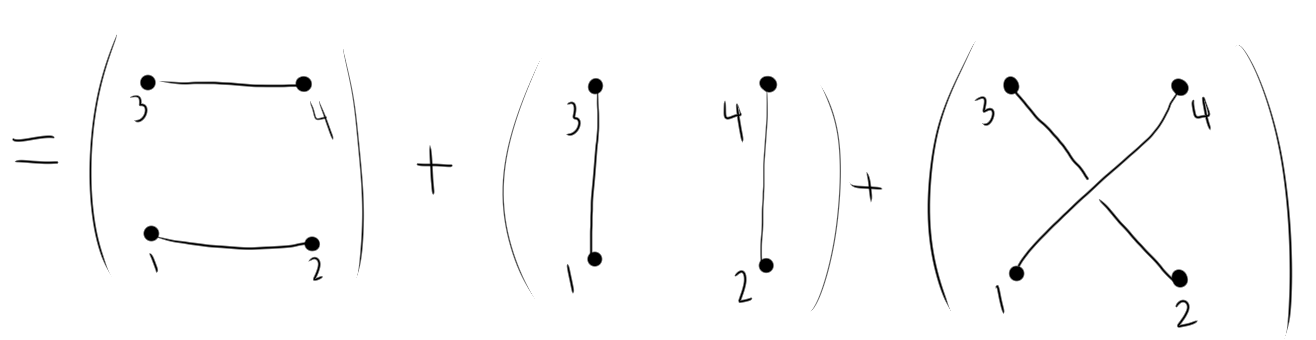
\includegraphics[scale=0.5]{images/feynman1.png}
	\caption{Feynman diagrams representing the nonzero values in the four particle example above.}
\end{figure}

\noindent Now stated in its general form \\

\noindent \textbf{Wick's Theorem}: $\mathcal{T}[\hat{\phi}_1 \dots \hat{\phi}_n] = \mathcal{N}[\hat{\phi}_1 \dots \hat{\phi}_n + \text{"all possible contractions"}]$. \\

\noindent \textbf{Proof:} \\
\noindent Induct on $n$, with the base case $n=2$ confirmed to be true, and check that the $n-1$ case implies the full $n$ case. \\
\noindent Assume, without loss of generality, that everything is time-ordered, such that $x_1^0 > x_2^0 > \dots > x_n^0$. \\
\noindent Then the left-hand side of Wick's theorem becomes
\begin{equation}
\mathcal{T}[\hat{\phi}_1 \dots \hat{\phi}_n] = \hat{\phi}_1 \hat{\phi}_2 \dots \hat{\phi}_n .
\end{equation}
\noindent Use the inductive hypothesis for $n-1$ case on this equation
\begin{align*}
\hat{\phi}_1 \hat{\phi}_2 \dots \hat{\phi}_n &= (\hat{\phi}_1^+ + \hat{\phi}_1^-) \mathcal{N} [ \hat{\phi}_2 \dots \hat{\phi}_n + \left(\text{\stackanchor{{\small all possible contractions}}{{\small excluding $\hat{\phi}_1$.}}}\right) ] \\
&= \hat{\phi}_1^+ \mathcal{N}[\hat{\phi}_2 \dots \hat{\phi}_n + \left(\text{\stackanchor{{\small all possible contractions}}{{\small excluding $\hat{\phi}_1$.}}}\right)] \\
&\,\,\,\,\,\, + \mathcal{N}[ \hat{\phi}_1^- \hat{\phi}_2 \dots \hat{\phi}_n + \hat{\phi}_1^- \left(\text{\stackanchor{{\small all possible contractions}}{{\small excluding $\hat{\phi}_1$.}}}\right) ] .
\end{align*}
\noindent Since $\hat{\phi}_1^-$ is already normal-ordered. \\
\noindent Focus on the first part of the first term of $\hat{\phi}_1 \hat{\phi}_2 \dots \hat{\phi}_n$ above
\begin{align*}
\hat{\phi}_1^+ \mathcal{N}[\hat{\phi}_2 \dots \hat{\phi}_n] &= \mathcal{N}[\hat{\phi}_2 \dots \hat{\phi}_n] \hat{\phi}_1^+ + [\hat{\phi}_1^+, \mathcal{N}[\hat{\phi}_2 \dots \hat{\phi}_n]] \\
&= \mathcal{N}[\hat{\phi}_1^+ \hat{\phi}_2 \dots \hat{\phi}_n] \\
&\,\,\,\, + \mathcal{N}[ [\hat{\phi}_1^+, \hat{\phi}_2]\hat{\phi}_3 \dots \hat{\phi}_n + \hat{\phi}_2 [\hat{\phi}_1^+,\hat{\phi}_3] \hat{\phi}_4 \dots \hat{\phi}_n + \dots + \hat{\phi}_2\hat{\phi}_3\dots\hat{\phi}_{n-1}[\hat{\phi}_1^+,\hat{\phi}_n]] \\
\hat{\phi}_1^+ \mathcal{N}[\hat{\phi}_2 \dots \hat{\phi}_n] &= \mathcal{N}[ \hat{\phi}_1^+ \hat{\phi}_2 \dots \hat{\phi}_n + \wick[offset=1.5em]{\c {\hat{\phi}_1^+} \c {\hat{\phi}_2} \hat{\phi}_3 \dots \hat{\phi}_n} + \wick[offset=1.5em]{\c {\hat{\phi}_1^+} {\hat{\phi}_2} \c {\hat{\phi}_3} \dots \hat{\phi}_n} + \dots + \wick[offset=1.5em]{\c {\hat{\phi}_1^+} {\hat{\phi}_2} \hat{\phi}_3 \dots \c {\hat{\phi}_n}} ] .
\end{align*}
\noindent Where the second equality follows from $[\hat{\phi}_j^\dagger, \hat{\phi}_k] \propto \mathbb{I}$. \\
\noindent Now, focus on the rest of the first term of $\hat{\phi}_1 \mathcal{N}[\hat{\phi}_2 \dots \hat{\phi}_n]$
\begin{align*}
\hat{\phi}_1^+ \mathcal{N}[ \left(\text{\stackanchor{{\small all possible contractions}}{{\small excluding $\hat{\phi}_1$.}}}\right) ] &= [ \hat{\phi}_1^+, \mathcal{N}[\dots]] + \mathcal{N}[\dots]\hat{\phi}_1^+ \\
&= \mathcal{N}[  \left(\text{\stackanchor{{\small all possible contractions}}{{\small including $\hat{\phi}_1^+$.}}}\right) ] + \mathcal{N}[\hat{\phi}_1^+ \left(\text{\stackanchor{{\small all possible contractions}}{{\small excluding $\hat{\phi}_1$.}}}\right)]
\end{align*}

\clearpage

\section{Lecture 10: Feynman Rules for $\varphi^4$ Theory}
\label{sec:lec10}

\noindent In perturbative, interacting field theories, we must calculate the $n$-point correlation function
\begin{equation}
G^{(n)}(x_1,\dots,x_n) = \frac{\bra{0} \mathcal{T} [\hat{\phi}_1 \dots \hat{\phi}_n \mathcal{S}]\ket{0}}{\bra{0} \mathcal{S} \ket{0}}
\end{equation}

\noindent Where the scattering matrix elements and the interacting Hamiltonian are
\begin{align}
\bra{\phi} \mathcal{S} \ket{\psi} &= \lim_{t\to\infty} \bra{\phi} \mathcal{T}[e^{-i\int^t_{-t} \hat{H}_I(t')dt'}] \ket{\psi} \\
\hat{H}_I(t) &= \frac{\lambda}{4!} \int d^3 x \,\hat{\phi}^4(\textbf{x})
\end{align}

\noindent The numerator and denominator of the correlation function must be expanded perturbatively in the small parameter $\lambda$. 
\begin{align}
G^{(n)} &= \frac{a_0 + \lambda a_1 + \lambda^2 a_2 + \dots}{b_0 + \lambda b_1 + \lambda^2 b_2 + \dots} \text{, where } a_j, b_j \in \mathbb{C} \\
&= \frac{1}{b_0} (a_0 + \lambda a_1 + \dots) (1 - \lambda \frac{b_1}{b_0} + \lambda^2 \frac{b_2}{b_0} + \dots) \\
&=_{\mathcal{O}(\lambda)} \frac{1}{b_0} (a_0 + \lambda a_1) (1-\lambda \frac{b_1}{b_0}) \\
G^{(n)} &= \frac{a_0}{b_0} + \lambda (\frac{a_1}{b_0} - \frac{b_1 a_0}{b_0^2}) \text{ to order } \lambda
\end{align}

\noindent This gives the intermediate task of calculating the coefficients of the perturbative expansion: $a_0$, $a_1$, $b_0$, and $b_1$. \\

\noindent Consider the $n=2$ case
\begin{equation}
G^{(2)}(x, y) = \lim_{t\to\infty} \frac{\bra{0} \mathcal{T} [\hat{\phi}(x) \hat{\phi}(y) e^{-i\int^t_{-t} \hat{H}_I(t')dt'}]\ket{0}}{\bra{0} \mathcal{T}[e^{-i\int^t_{-t} \hat{H}_I(t')dt'}]\ket{0}}
\end{equation}

\noindent Expand the exponentials, keeping to order $\lambda$, and insert into numerator. The numerator is then
\begin{align}
\bra{0} \mathcal{T} [\hat{\phi}(x) \hat{\phi}(y) \mathcal{S}]\ket{0} &= \bra{0} \mathcal{T} [\hat{\phi}(x) \hat{\phi}(y) e^{-i\int^t_{-t} \hat{H}_I(t')dt'}]\ket{0} \\
&= \bra{0} \mathcal{T} [\hat{\phi}(x) \hat{\phi}(y) \left( \mathbb{I} - \frac{i\lambda}{4!} \int d^4 z \, \hat{\phi}^4(z) \right)]\ket{0} \\
&= \bra{0} \mathcal{T} [\hat{\phi}(x) \hat{\phi}(y)] \ket{0} - \frac{i\lambda}{4!} \int d^4 z \, \bra{0} \mathcal{T} [\hat{\phi}(x) \hat{\phi}(y) \hat{\phi}^4(z)] \ket{0} \\
\bra{0} \mathcal{T} [\hat{\phi}(x) \hat{\phi}(y) \mathcal{S}]\ket{0} &= \Delta_F(x-y) - \frac{i\lambda}{4!} \int d^4 z \, \bra{0} \mathcal{N} [\hat{\phi}(x) \hat{\phi}(y) \hat{\phi}^4(z) + \text{all contractions}] \ket{0}
\end{align}

\noindent The last line is gotten by applying Wick's theorem, and recall that any terms with \textit{uncontracted} operators will evaluate to \textbf{zero} in the vacuum expectation value (e.g., $\bra{0}\mathcal{N}[\dots]\ket{0}$), and only the \textit{fully contracted} terms will contribute, such as $\bra{0}\wick[offset=1.5em]{\c1 {\hat{\phi}(x)} \c2 {\hat{\phi}(y)} \c3 {\hat{\phi}(z)} \c2 {\hat{\phi}(z)} \c1 {\hat{\phi}(z)} \c3 {\hat{\phi}(z)}}\ket{0}$, and $\bra{0}\wick[offset=1.5em]{\c1 {\hat{\phi}(x)} \c1 {\hat{\phi}(y)} \c2 {\hat{\phi}(z)} \c2 {\hat{\phi}(z)} \c3 {\hat{\phi}(z)} \c3 {\hat{\phi}(z)}}\ket{0}$. \\

\noindent Now, "all good physics and math ends in linear algebra, combinatorics, or both", and we use combinatorics to calculate how many fully contracted terms we expect to see in the expansion. 
\begin{itemize}
\item There are $(2n-1)!!$ full contractions per expansion, where $n$ is the number of unique particles. In this case, $n=3$ for $x$, $y$, and $z$ spacetime coordinates.
\item There are 2 unique contraction types out of the $(2\cdot3-1)!! = 15$ full contractions.
	\subitem $\Delta_F(x-y) \Delta_F^2(z-z)$
	\subitem $\Delta_F(x-z) \Delta_F(y-z) \Delta_F(z-z)$
\item There are 3 contractions of the first type
	\subitem Connect $x\to y$ in 1 way and $z\to z$ twice, each in only 1 way.
\item There are 12 contractions of the second type
	\subitem Connect $x\to z$ in 4 ways, followed by $y\to z$ in 3 ways, and $4\cdot 3=12$.
\end{itemize}

\noindent Return to the numerator of the correlation function, and pretending that $\Delta_F(z-z)$ is finite, for now,
\begin{align*}
\bra{0} \mathcal{T} [\hat{\phi}(x) \hat{\phi}(y) \mathcal{S}]\ket{0} &= \Delta_F(x-y) \\
&\,\,\,\,\,\, + \left(-\frac{i\lambda}{4!}\right) \int d^4 z \, \bra{0} \mathcal{N} [\cancel{\hat{\phi}(x) \hat{\phi}(y) \hat{\phi}^4(z)} + \cancel{\text{\tiny {\stackanchor{all partial}{contractions}}}} + \text{\tiny {\stackanchor{all full}{contractions}}}] \ket{0} \\
&= \Delta_F(x-y) + 3 \cdot \left(-\frac{i\lambda}{4!}\right)\int d^4 z \, \Delta_F(x-y) \Delta_F^2(z-z) \\
&\,\,\,\,\,\, + 12 \cdot \left(-\frac{i\lambda}{4!}\right)\int d^4 z \, \Delta_F(x-z) \Delta_F(y-z) \Delta_F(z-z)
\end{align*}

\noindent And in diagrammatic form

\begin{figure}[H]
	\centering
	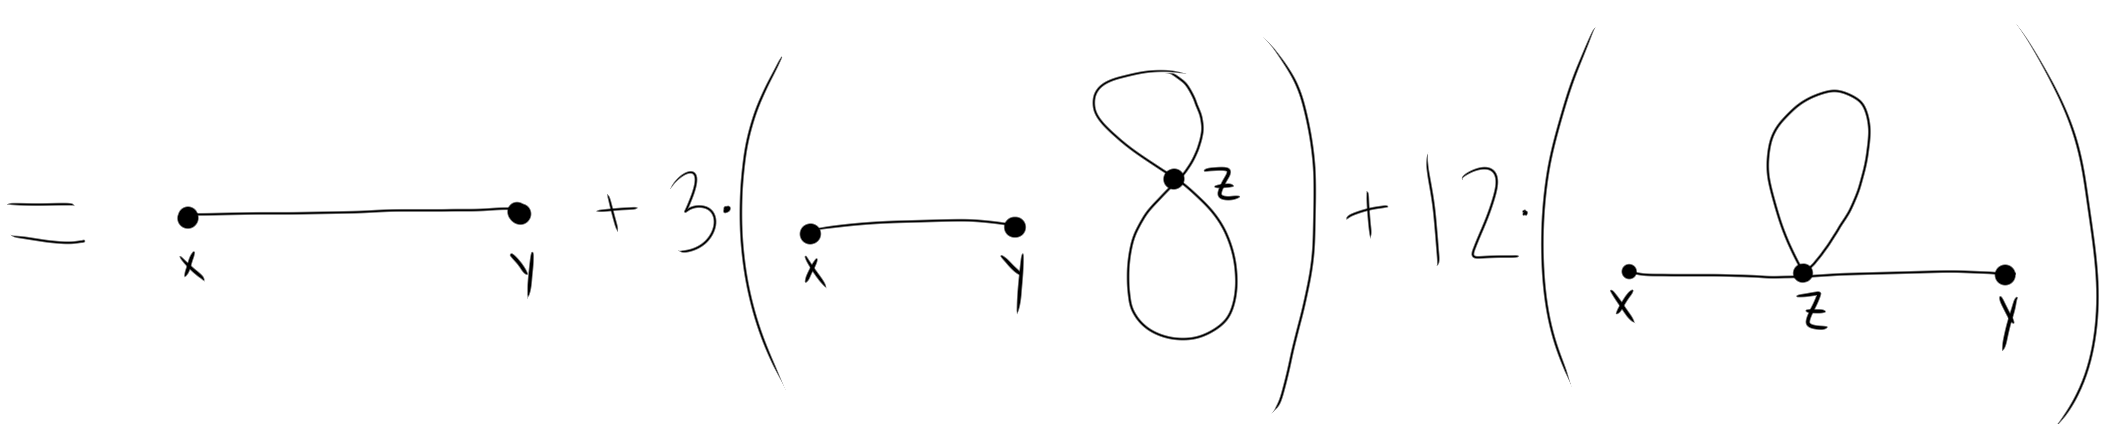
\includegraphics[scale=0.3]{images/feynman2.png}
	\caption{Feynman diagram representation of the above integral values for the $\varphi^4$ interacting theory.}
\end{figure}

\noindent Similarly calculate the denominator of the two-point correlation function to obtain the following

\begin{figure}[H]
	\centering
	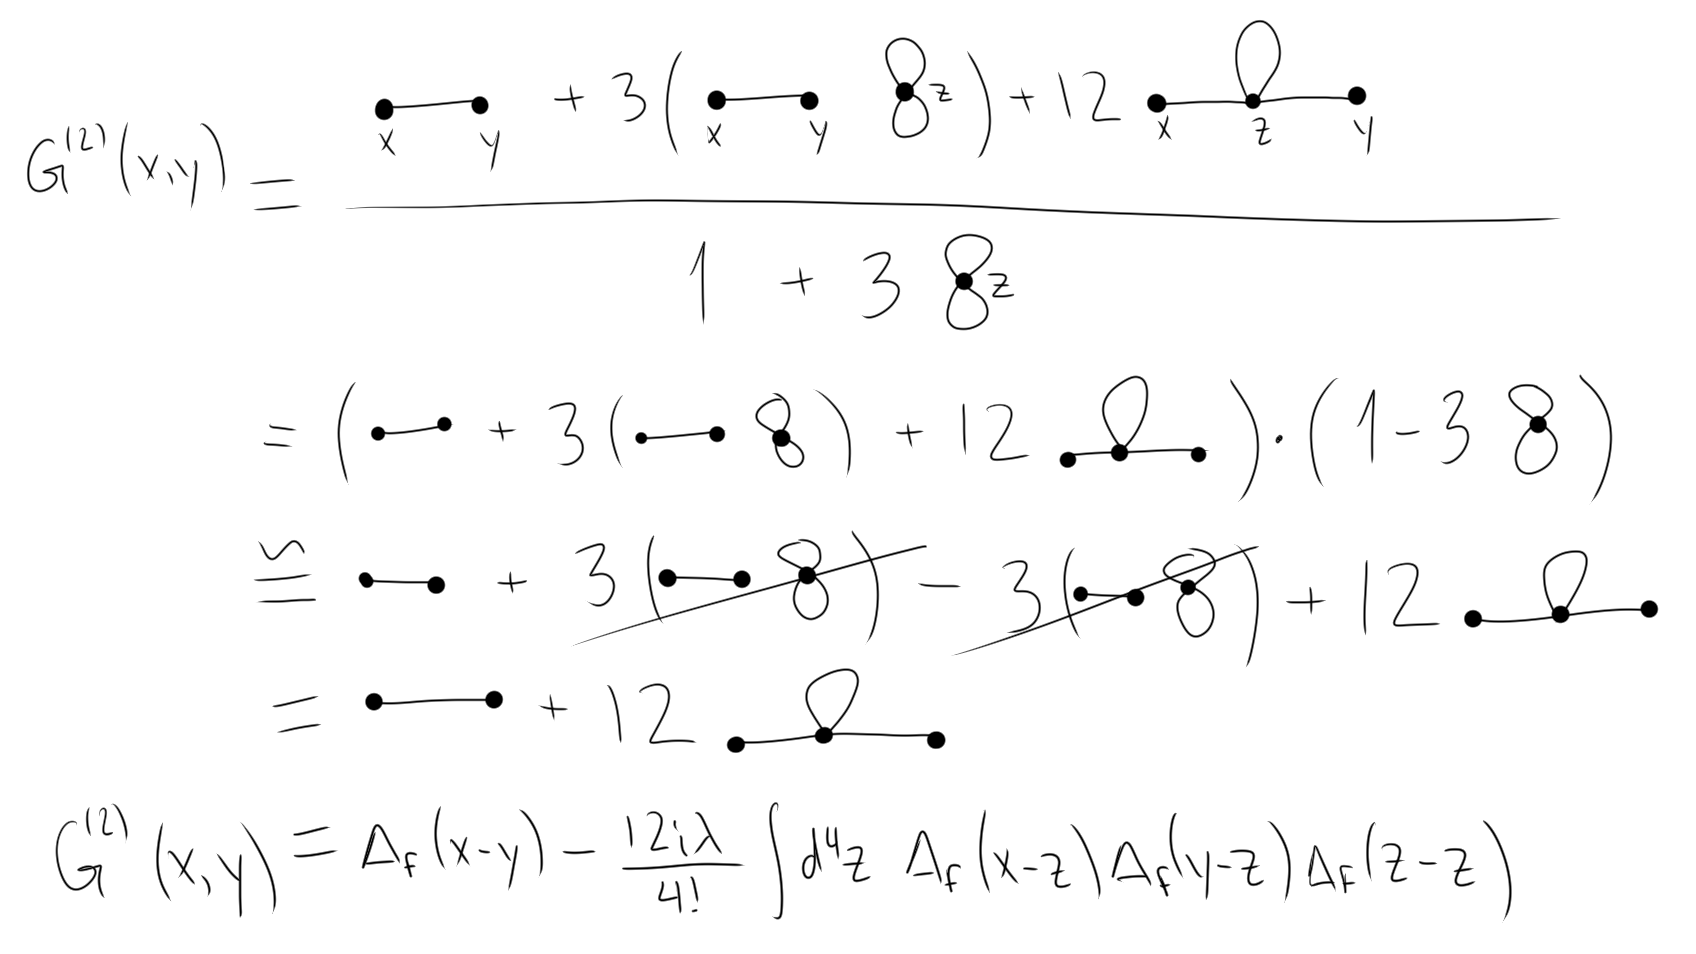
\includegraphics[scale=0.4]{images/twopoint.png}
	\caption{Feynman diagram calculation for the two-point correlation function for the $\varphi^4$ theory. Note that this "miraculous" cancellation of divergent terms (the "self-interacting figure-eight") actually follows from a more general result.}
\end{figure}

\noindent The arguments of the correlation function are the \textbf{external vertices}, and the spacetime coordinates of the interacting Hamiltonian are the \textbf{internal vertices}.

\noindent To calculate the value of a diagram, associate a factor, the Feynman propagator, $\Delta_F(x-y)$ to each edge connecting external vertices (e.g., $x$ and $y$), and associate the factor $-i\lambda \int d^4 z$ (dividing by the symmetry factor $4!$) to each internal vertex (e.g., $z$). \\

\noindent For example,

\begin{figure}[H]
	\centering
	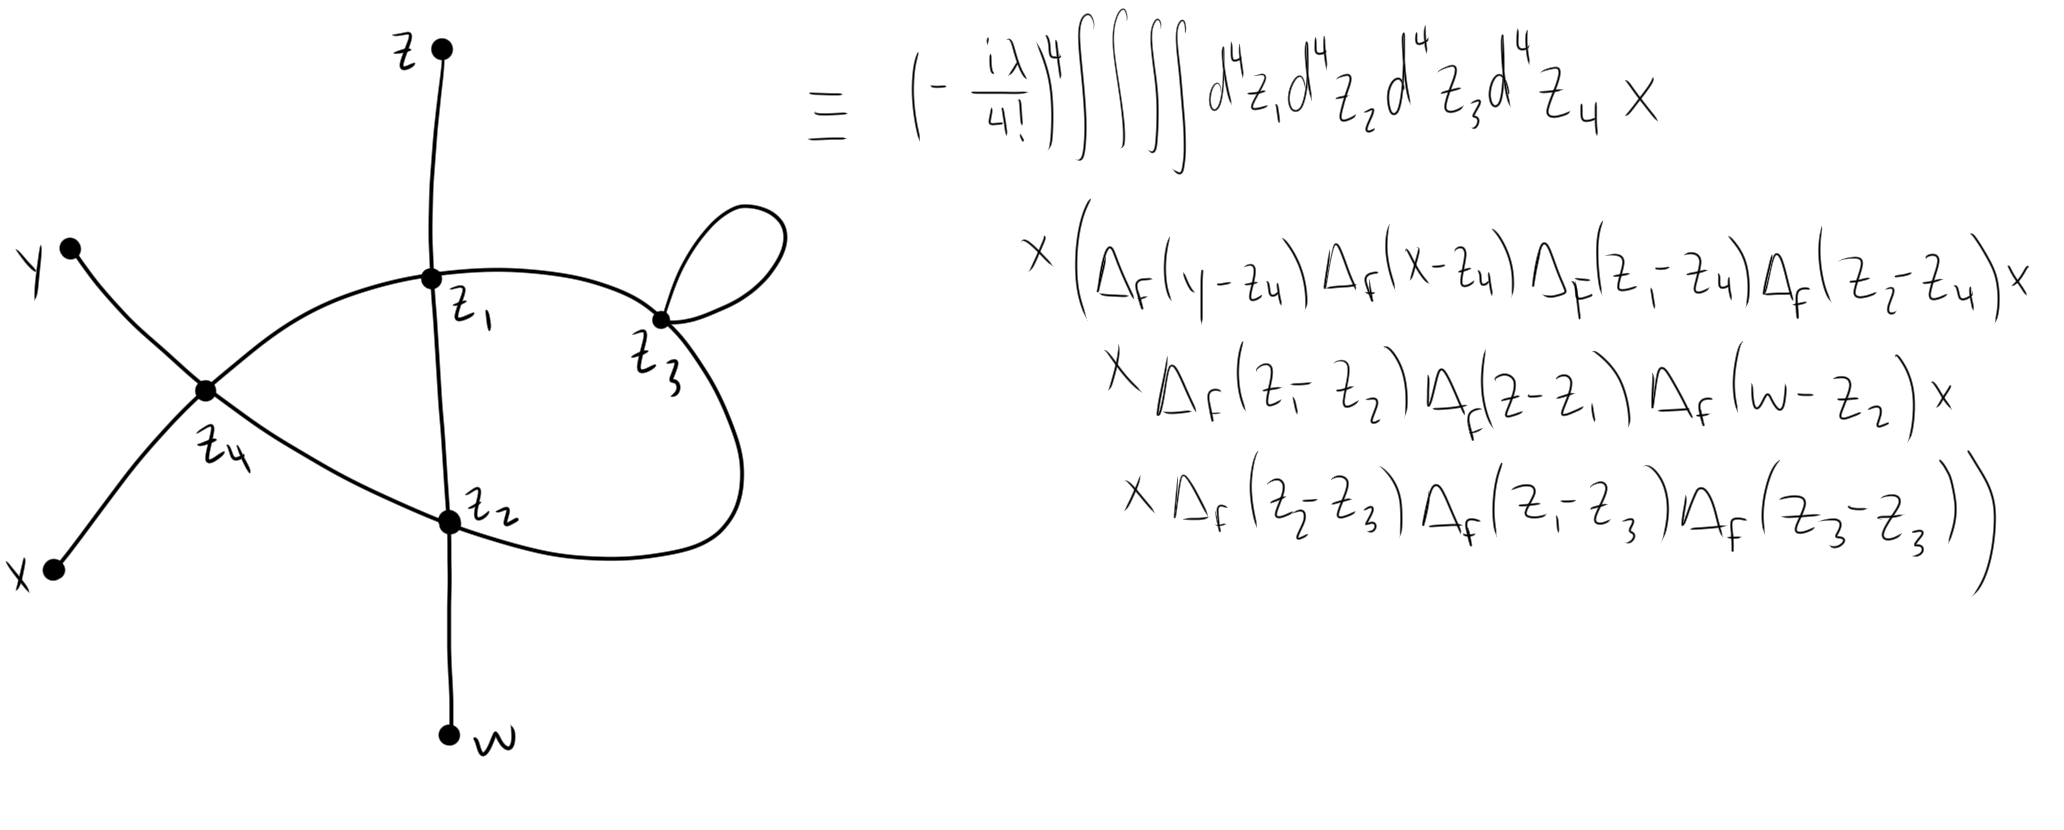
\includegraphics[scale=0.3]{images/4int4ext.png}
	\caption{Example Feynman diagram and associated values with 4 external vertices and 4 internal vertices.}
\end{figure}

\noindent In summary, to calculate $G^{(2)}(x,y)$ to arbitrary order, sum over all possible diagrams with 2 external vertices, subject to the (canonical) Feynman rules for $\varphi^4$ theory.

\begin{equation}
G^{(2)}(x,y) = \frac{\bra{0}\mathcal{T}[\hat{\phi}(x)\hat{\phi}(y)\mathcal{S}]\ket{0}}{\bra{0}\mathcal{S}\ket{0}} = \left(\text{\small {\stackanchor{sum of all possible diagrams}{with two external vertices}}}\right)
\end{equation}

\begin{figure}[H]
	\centering
	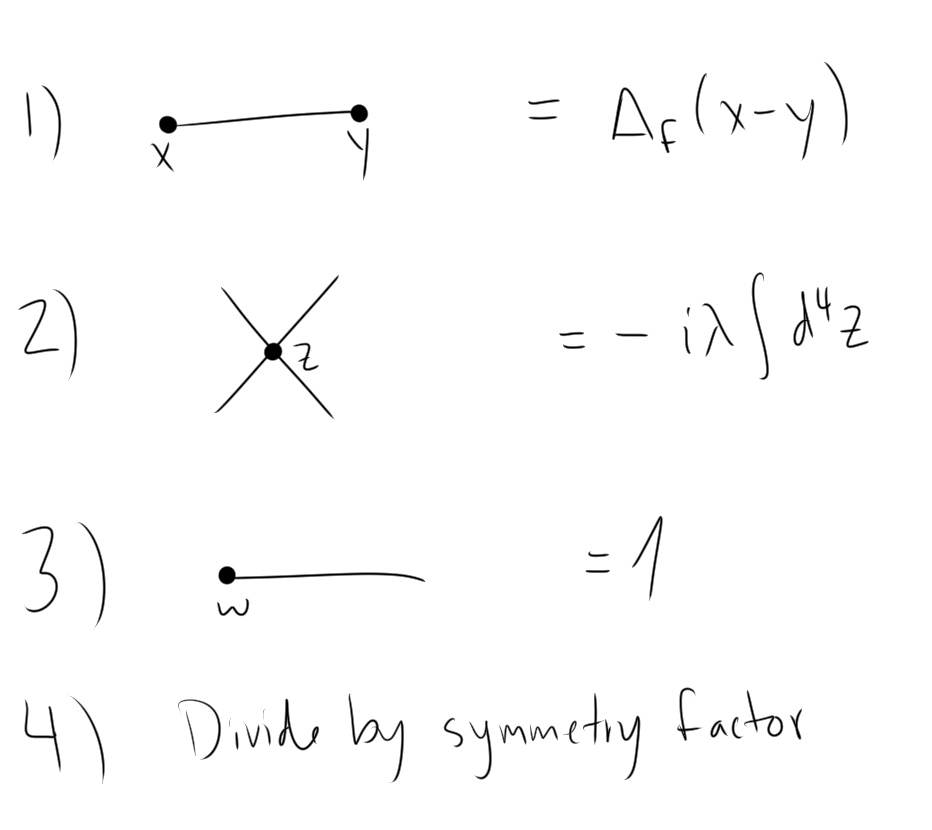
\includegraphics[scale=0.5]{images/phi4rules.png}
	\caption{\textbf{Canonical Feynman rules for $\varphi^4$ theory}.}
\end{figure}

\noindent Note the abscence of the inverse $4!$ factor in rule number 2, as it is added based on observation, and not considered a component on the \textit{canonical} rules. \\

\noindent Higher order terms in the expansion of the two-point correlation function become successively more complicated and often redundant. For example, The self-interacting "figure-eight" diagram of an internal vertex can occur in $4!\cdot8=192$ ways. The redundancy is encoded in the \textbf{symmetry factor} (see rule 4 above) of the diagram. Typically, in practice and computation, distinct diagrams are written down and overcounting is determined via the symmetry factor.

\clearpage

\section{Lecture 11: Feynman Rules and Vacuum Bubbles}
\label{sec:lec11}

\noindent The Feynman rules demonstrated in the last lecture are specifically for the $\varphi^4$ theory of interacting quantum fields in \textit{position space}, and allow the calculation of $n$-point correlation (Green's) functions, which are not directly observable, but related to scattering amplitudes which are directly observable. We did not rigorously prove, but demonstrated (with $n=2$) the feasibility of and accepted as "definition", that the $n$-point correlation function is equal to the sum of all possible diagrams with $n$ external vertices, subject to the Feynman rules in position space. Keep note that we did not consider $n>2$ or $\lambda>1$ in the following equality.
\begin{align}
G^{(n)}(x_1,\dots,x_n) &= \frac{\bra{0}\mathcal{T}[\hat{\phi}(x_1) \dots \hat{\phi}(x_n)\mathcal{S}]\ket{0}}{\bra{0}\mathcal{S}\ket{0}} \\
&= \left(\text{\small {\stackanchor{sum of all possible diagrams with $n$ external vertices}{subject to Feynman rules in position space}}}\right)
\end{align}

\noindent A ubiquitous issue and deep concern in quantum field theory is the appearance infinities in calculations. Nature seems to suggest that there are no infinities, unless one asks the wrong question. (Are there actually any physical quantities that can be proven to be infinite by experiment, such as the energy levels of the hydrogen atom or the results of continuous scattering theory?) Many infinities that appear due to the application of the Feynman rules will be trivially dispelled (\textit{cf.}, in quantum mechanics when an infinite ground state energy is calculated, simply apply a shift to make it finite). \textbf{Vacuum bubbles} are diagrams with no external vertices (e.g., self interactions) that evaluate to infinity, but will cancel in calculating the $n$-point correlation function $G^{(n)}(x_1,\dots,x_n)$, as we saw in the $n=2$ case in the last lecture.\\

\subsection*{Feynman Rules in Momentum Space ($\varphi^4$ Theory)}

\noindent Remember that the perturbation expansion of the $\mathcal{S}$-matrix and the Green's function can be calculated in momentum space via the Feynman rules in momentum space. The momentum space Feynman propagator has the form
\begin{equation}
\Delta_F(x,y) = \int \frac{d^4 p}{(2\pi)^4} \frac{i e^{-i p \cdot (x-y)}}{p^2-m^2 + i\epsilon}
\end{equation}

\noindent Calculating the perturbation expansion in momentum space may make additional cancellations more apparent. The Feynman rules for $\varphi^4$ theory in momentum space are as follows
\begin{enumerate}
\item For each propagator with momentum $p$, add a factor of $\frac{i}{p^2-m^2+i\epsilon}$.
\item For each (internal) vertex, add a factor of $-i\lambda$.
\item For each external vertex, add a factor of $e^{-ip\cdot x}$.
\item Impose momentum conservation at each vertex.
\item Integrate over undetermined momenta.
\item Divide by symmetry factor.
\end{enumerate}

\begin{figure}[H]
	\centering
	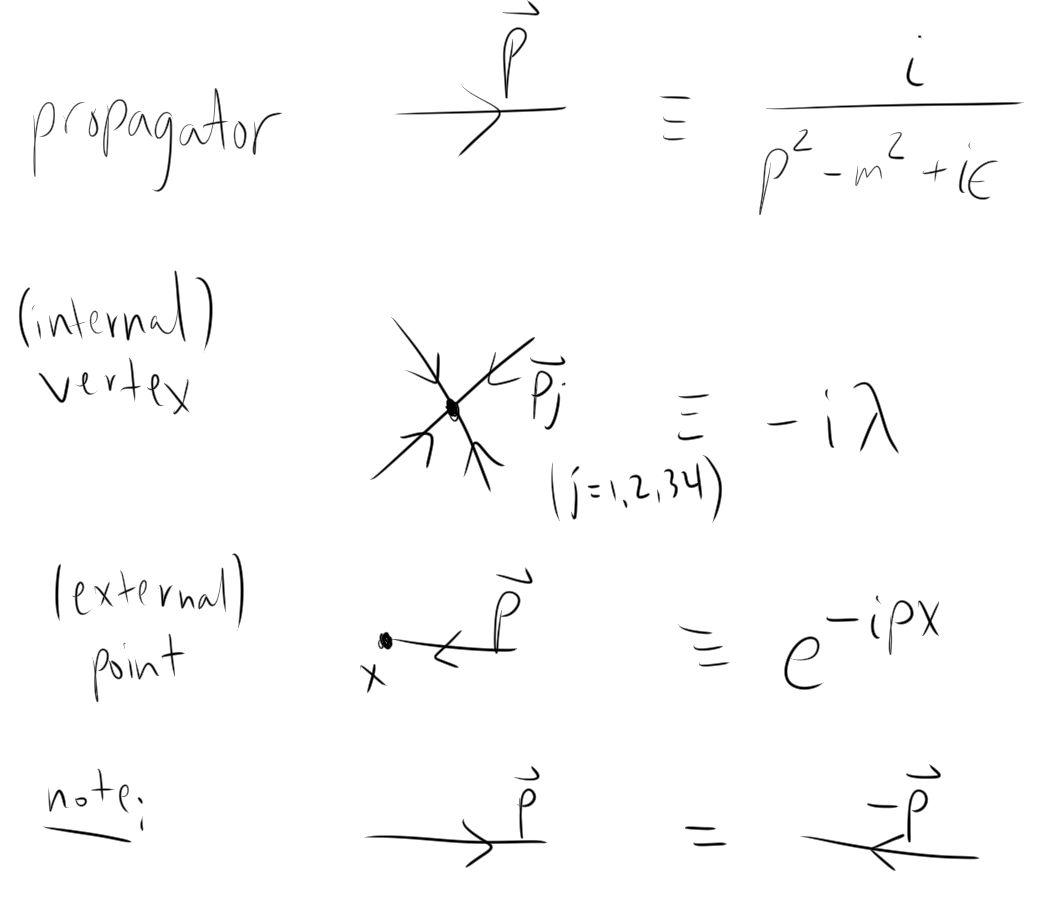
\includegraphics[scale=0.6]{images/feynmanmom.png}
	\caption{Diagrammatic representation for the Feynman rules in momentum space.}
\end{figure}

\noindent Returning to the $n=2$ case, a general diagram consists of a product of \textit{connected} components and \textit{disconnected} components. Note that the external vertices ($x$ and $y$ in the $n=2$ case) are always connected, since their degrees are odd. For example,

\begin{figure}[H]
	\centering
	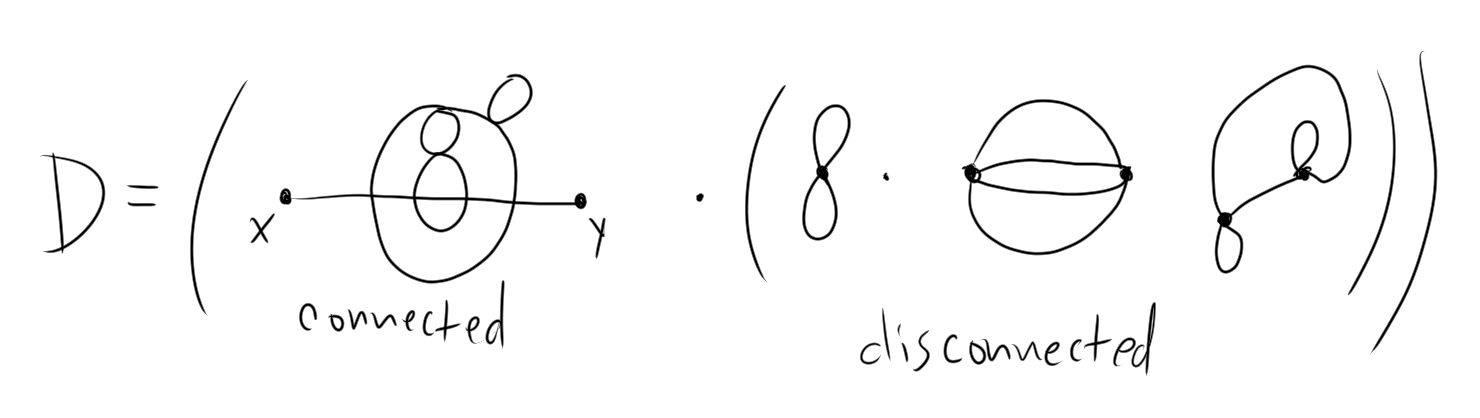
\includegraphics[scale=0.4]{images/n2diagrams.png}
	\caption{Typical diagram for $n=2$ case.}
\end{figure}

\noindent All possible disconnected pieces form a countable set. 

\begin{figure}[H]
	\centering
	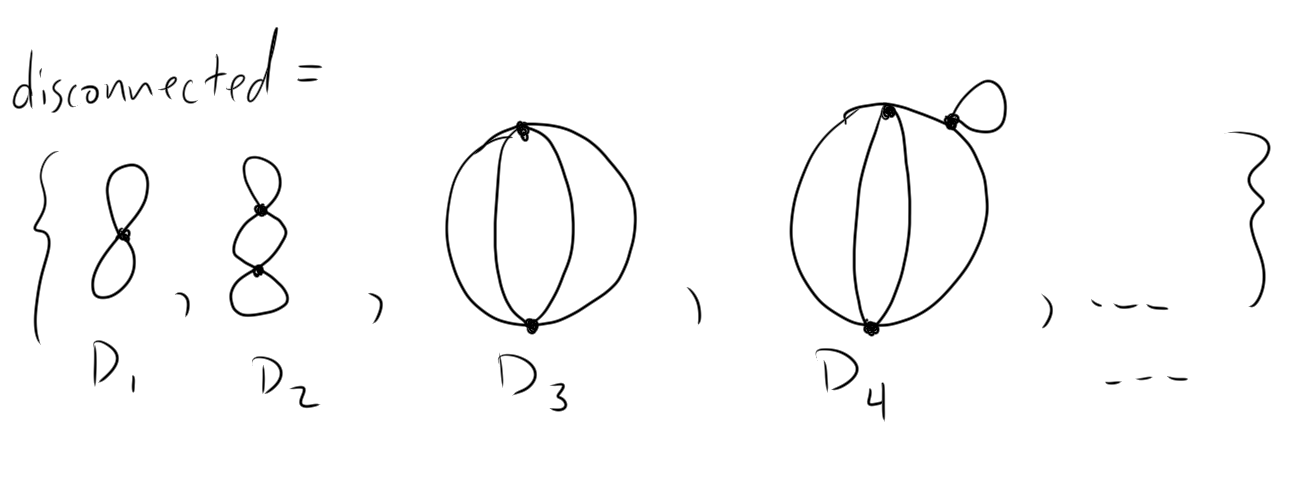
\includegraphics[scale=0.4]{images/countable.png}
	\caption{Countable set of all possible disconnected pieces.}
\end{figure}

\noindent Each type of disconnected diagram $D_j$ has a unique value $v(D_j)=v_j$, which are all \textit{infinite}. To interpret this result, place a \textbf{cutoff} on the theory. It must be checked that the results, after evaluating the diagrams of the expansion, do not depend on the cutoff imposed. \\

\noindent Suppose that a given diagram $D$ has $n_j$ components of type $D_j$, including the connected component. The value of the diagram is the product of the values of the connected and disconnected components.
\begin{equation}
v_j = v_{connected} \cdot \prod_{j=1}^{\infty} \frac{1}{n_j !} v_j^{n_j}
\end{equation}

\noindent Where $n_j !$ is the symmetry factor. \\

\noindent For the $n=2$ diagram example above, we have the product of the connected piece with disconnected types $D_1$, $D_3$, and $D_2$, respectively, with $n_j=1$ for each diagram type $j$. Therefore the value of the diagram is
\begin{equation}
v(D) = v_{connected} \cdot v_1 \cdot v_3 \cdot v_2
\end{equation}

\begin{figure}[H]
	\centering
	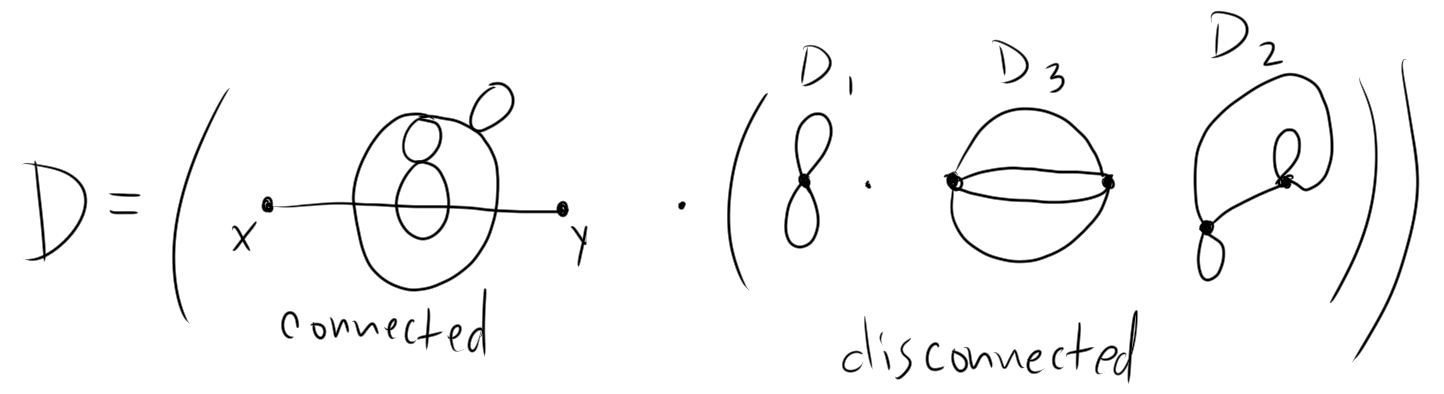
\includegraphics[scale=0.4]{images/n2diagramslabel.png}
	\caption{Typical diagram for $n=2$ case with disconnected pieces labelled by type.}
\end{figure}

\noindent This allows us to write down a more closed form for the series expansion for $G^{(2)}(x,y)$, and ditch the "all possible diagrams" bit. The numerator of $G^{(2)}(x,y)$ is then
\begin{align}
\text{Numerator(}G^{(2)}(x,y)\text{)} &= \sum_{connected} \sum_{\{n_j\}} v_{connected} \cdot \prod_{j=1}^\infty \frac{1}{n_j !} v_j^{n_j} \\
&= \sum_{conn.} v_{conn.} \sum_{\{n_j\}} \prod_{j=1}^\infty \frac{1}{n_j !} v_j^{n_j} \\
&= \sum_{conn.} v_{conn.} \prod_{j=1}^\infty \sum_{\{n_j\}} \frac{1}{n_j !} v_j^{n_j}  \\
\text{Numerator(}G^{(2)}(x,y)\text{)} &= \sum_{conn.} v_{conn.} \cdot e^{\sum_{j=1}^{\infty} v_j}
\end{align}

\noindent Note that we justify these manipulations of not-necessarily-convergent series by the implemented cutoff, which makes each value finite. Similarly, the denominator is simply the sum over the same exponential
\begin{equation}
\text{Denominator(}G^{(2)}(x,y)\text{)} = e^{\sum_{j=1}^{\infty} v_j}
\end{equation}

\noindent This cancels exactly with the same term in the numerator, pulled out of the sum over connected parts. Therefore, the $2$-point correlation function, which generalizes to $n>2$, is equal to the sum of all connected components subject to the Feynman rules.
\begin{equation}
G^{(2)}(x,y) = \left(\stackanchor{sum over all connected diagrams}{subject to Feynman rules}\right)
\end{equation}

\begin{figure}[H]
	\centering
	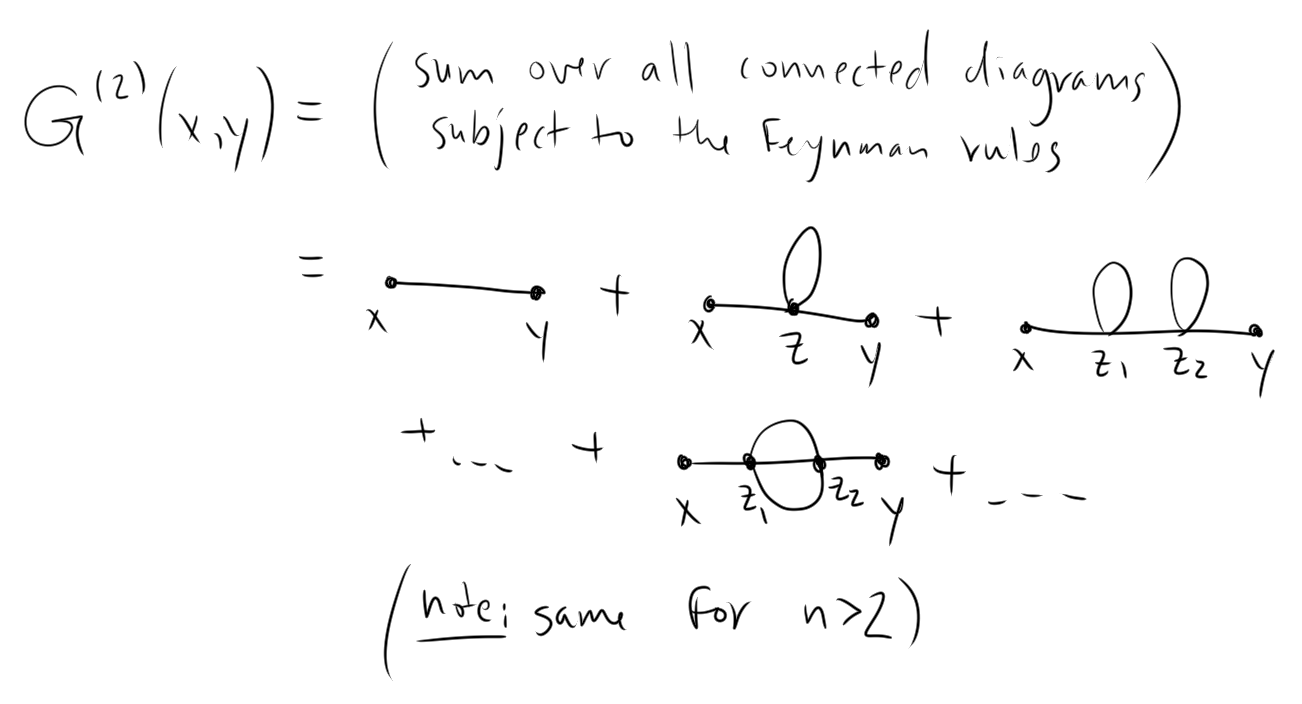
\includegraphics[scale=0.6]{images/allconnected.png}
	\caption{The sum over all connected diagrams subject to the Feynman rules.}
\end{figure}

\subsection*{Cutoffs in QFT}

\noindent Consider the Klein-Gordon Hamiltonian
\begin{equation}
\hat{H}_{KG} = \frac{1}{2} \int d^3 x \left( \hat{\pi}^2(x) + (\nabla \hat{\phi} (x))^2 + m^2 \hat{\phi}^2(x) \right)
\end{equation}

\noindent This assumes an infinitie number of degrees of freedom, one per each point in spacetime $x \in \mathcal{M}_4$. Now, for example, our theory and understanding of spacetime breaks down below the Planck scale. We can either continue to work in ignorance, or remember that we are dealing in \textit{effective} theories that, hopefully, represent something more fundamental. For example, the Navier-Stokes equation is an effective theory for quantum chromodynamics (QCD). An \textbf{effective theory} is a description which explains all observations up to a given scale $s$, often expressed in inverse length, and may break down beyond the given scale. \\

\noindent To impose a cutoff on the Hamiltonian, add a "fixing" term $\hat{H}_\Lambda$ which is well-behaved up to the scale $\Lambda$, and must match predictions of the original Hamiltonian $\hat{H}$
\begin{equation}
\hat{H} \to \hat{H}' = \hat{H} + \hat{H}_\Lambda
\end{equation}

\noindent To modify the new Hamitonian for other scales, Wilson's \textbf{renormalization theory} may be used, where the "fixing" Hamiltonian $\hat{H}_\Lambda$ is parameterized by the field operators and their derivatives
\begin{align}
\hat{H}_\Lambda &= \sum_{polynomials} \mathcal{P}(\hat{\phi}, \nabla \hat{\phi}, \nabla^2 \hat{\phi}, \dots, \hat{\pi}, \nabla \hat{\pi}, \nabla^2 \hat{\pi}, \dots) \\
&= c_0 \hat{\phi} + c_1 \hat{\phi}^2 + \dots + d_0 \hat{\pi} + d_1 \hat{\pi}^2 + \dots + e_1 (\nabla \hat{\phi})^2 + \dots
\end{align}

\noindent Only a finite number of the coefficients are nonzero and have an effect on observations beyond the scale $\Lambda$. By effect, the value of the term in the sum over field operator polynomials is not suppressed by inverse powers of $\Lambda$. Such terms that are not suppressed and have an effect on observations are called \textbf{relevant terms}. Any cutoff that is imposed must differ only by relevant terms. \\

\noindent For example, the relevant terms up to 4 dimensions is 
\begin{equation}
\{ \hat{\phi}, \hat{\phi}^2, \nabla^2 \hat{\phi}, \hat{\pi}, \hat{\pi}^2, \hat{\phi}^3, \hat{\phi}^4 \}.
\end{equation}

\noindent The simplest cutoff to impose on the momentum states of the free Klein-Gordon Hamiltonian is
\begin{equation}
\hat{H}_{KG} = \int \frac{d^3 p}{(2\pi)^3} \omega_p \hat{a}_p^\dagger \hat{a}_p \to \hat{H}_{KG}+\hat{H}_\Lambda = \int_{|p|<\Lambda} \frac{d^3 p}{(2\pi)^3} \omega_p \hat{a}_p^\dagger \hat{a}_p
\end{equation}

\noindent And the simplest cutoff for $\varphi^4$ interaction is
\begin{equation}
\hat{H}_{\varphi^4} = \frac{\lambda}{4 !} \int d^3 x \, \hat{\phi}^4(x) \to \hat{H}_{\varphi^4} + \hat{H}_\Lambda = \int_{|p_j|<\Lambda} d^3 p_1 d^3 p_2 d^3 p_3 d^3 p_4 (\dots)
\end{equation}

\noindent The new Hamiltonian for the quantum Klein-Gordon field with $\varphi^4$ interactions, and an imposed cutoff at scale $\Lambda$ is then written as
\begin{align}
\hat{H} \to \hat{H'} &= \hat{H}_{KG} + \hat{H}_{\varphi^4} + \hat{H}_\Lambda \\
&= \int_{|p|<\Lambda} \frac{d^3 p}{(2\pi)^3} \omega_p \hat{a}_p^\dagger \hat{a}_p + \int_{|p_j|<\Lambda} d^3 p_1 d^3 p_2 d^3 p_3 d^3 p_4 (\dots)
\end{align}

\clearpage

\section{Lecture 12: The $\mathcal{S}$-matrix in $\varphi^4$ Theory}
\label{sec:lec12}

\noindent Recall that some diagrams evaluate to infinity in the calculation of the time-ordered $n$-point correlation function
\begin{equation}
G^{(n)}(\textbf{x}_1,\dots,\textbf{x
}_n) = \bra{\Omega} \mathcal{T}[\hat{\phi}(\textbf{x}_1) \dots \hat{\phi}(\textbf{x}_n) ] \ket{\Omega} = \left( {\tiny \stackanchor{sum over all connected diagrams}{with $n$ external points/legs} } \right)
\end{equation}

\subsection*{Example: $n=4$ Diagrams}

\noindent For example, the $n=4$ case sums over diagrams like the following

\begin{figure}[H]
	\centering
	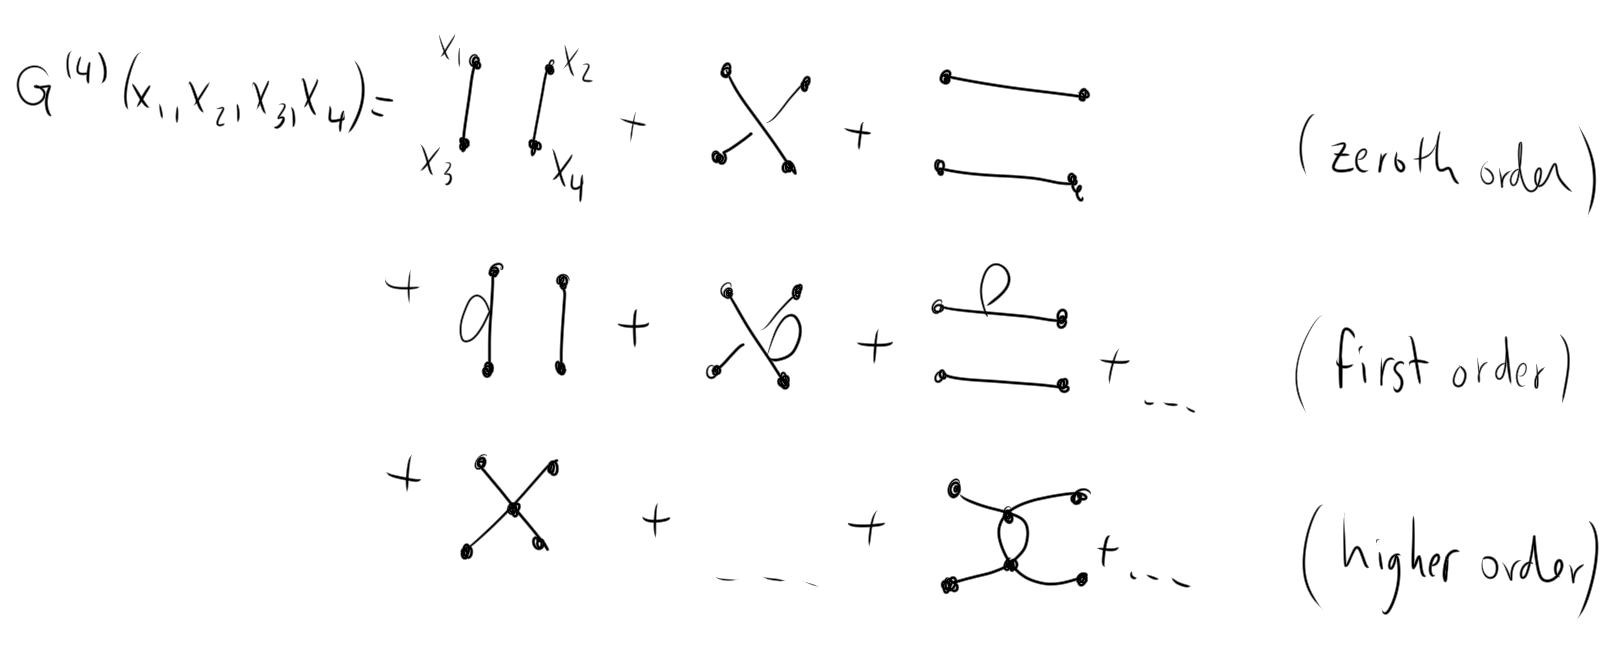
\includegraphics[scale=0.4]{images/g4.png}
	\caption{Sum over connected diagrams for $n=4$ case.}
\end{figure}

\noindent Diagrams with one loop (\textit{first order}) evaluate to infinity, but are easily eschewed. Two vertex diagrams (last one in figure above) is a much more difficult infinity to tame, and causes divergences, typically of the form, in momentum space,
\begin{equation}
\mathcal{I} = \int \frac{d^4 p} {(2\pi)^4} \, \frac{i}{\textbf{p}^2-m^2+i\epsilon}
\end{equation}

\noindent To attempt to tame the infinity, impose a cutoff at scale $\Lambda$
\begin{equation}
\mathcal{I} \to \mathcal{I}(\Lambda) = \int_{|p| < \Lambda} \frac{d^4 p} {(2\pi)^4} \, \frac{i}{\textbf{p}^2-m^2+i\epsilon} .
\end{equation}

\noindent To cope with arbitrary choices of $\Lambda$, arbitrary coupling constants can be employed to compensate and remove possible $\Lambda$-dependencies in calculations. Further explanation can be found in the renormalization theory of scalar particles.

\subsection*{Scattering Theory}

\noindent Scattering theory is an effective theory for large time limits $|t| >> \text{constant}$. The probability of a scattering event occuring, the scattering amplitude, in the case of well-collimated beams with incoming momenta $\textbf{k}_A$ and $\textbf{k}_B$, and outgoing momenta $\textbf{p}_j, \, j=1,\dots,n$, is related to the quantity
\begin{equation}
_{out}\braket{\textbf{p}_1 \textbf{p}_2 \dots \textbf{p}_n | \textbf{k}_A \textbf{k}_B}_{in} = \bra{\textbf{p}_1 \textbf{p}_2 \dots \textbf{p}_n} \mathcal{S} \ket{\textbf{k}_A \textbf{k}_B} .
\end{equation}

\begin{figure}[H]
	\centering
	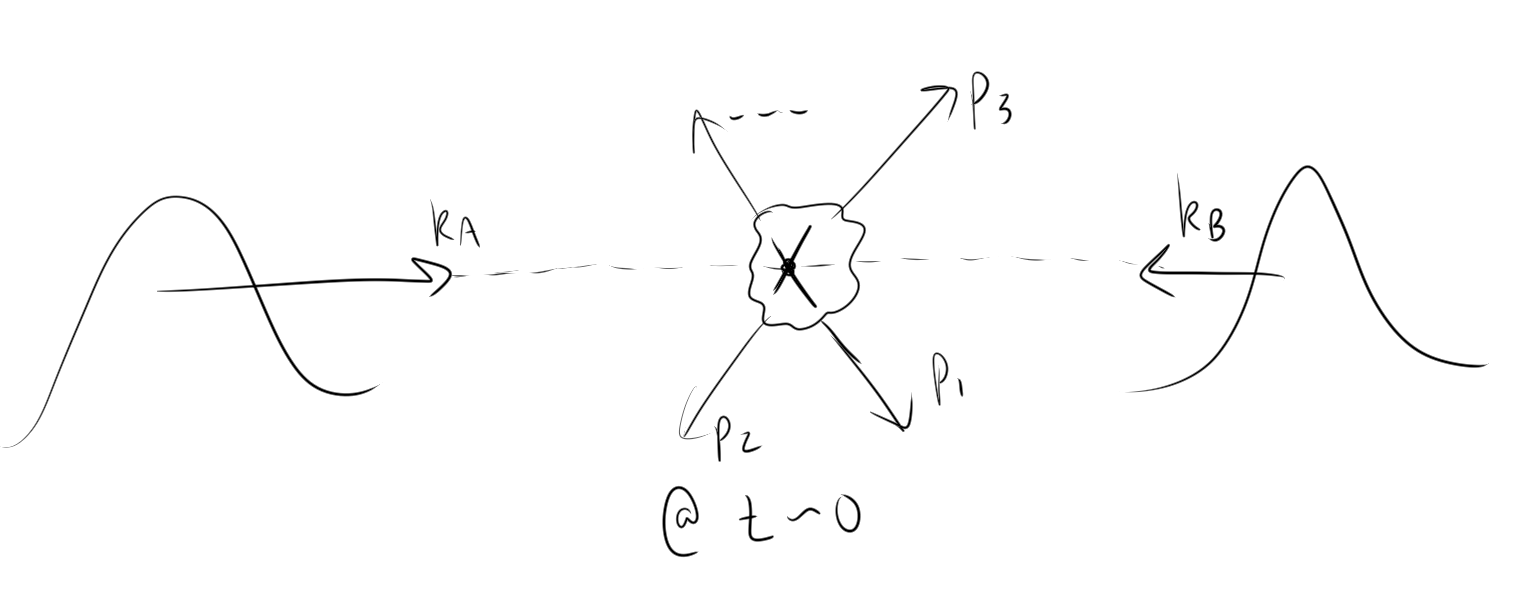
\includegraphics[scale=0.4]{images/scattering.png}
	\caption{Schematic of scattering experiment with incoming momenta and outgoing momenta as described above.}
\end{figure}

\noindent For the free, non-interacting, theory, we have the equation for incoming momenta related to the free vacuum state, denoted by $\ket{\,}_0$,
\begin{equation}
\ket{k_A k_B}_{in} = \sqrt{2 \omega_{k_A} \omega_{k_B}} \hat{a}_{k_A}^\dagger \hat{a}_{k_B}^\dagger \ket{0}_0 .
\end{equation}

\noindent The task at hand is to calculate the scattering amplitude $\bra{\textbf{p}_1 \textbf{p}_2 \dots \textbf{p}_n} \mathcal{S} \ket{\textbf{k}_A \textbf{k}_B}$. Define the $\mathcal{S}$-matrix as
\begin{equation}
\mathcal{S} = \mathbb{I} + i \hat{\mathbb{T}}.
\end{equation}

\noindent Where the identity $\mathbb{I}$ is the dominant term in small intercation, where almost nothing happens, and the operator $\hat{\mathcal{T}}$ is the dominant in larger interactions. Introduce the quantity $\mathcal{M}$ to factor out the conservation of momentum in the scattering process, where all momenta are "on shell", such that $\textbf{p}^0 = \omega_p$. 
\begin{equation}
\bra{\textbf{p}_1 \dots \textbf{p}_n} i\hat{\mathbb{T}} \ket{\textbf{k}_A \textbf{k}_B} = (2\pi)^4 \delta^{(4)}((\textbf{k}_A + \textbf{k}_B) - \sum_{j=1}^{n} p_j) \cdot i \mathcal{M}((\textbf{k}_A, \textbf{k}_B) \to \textbf{p}_f).
\end{equation}

\noindent Recall that the differential scattering cross section of $2\to 2$ particles in the center of mass frame is
\begin{equation}
\left( \frac{d\sigma}{d\Omega}\right)_{CM} = \frac{|\mathcal{M}|^2}{64 \pi^2 E^2_{CM}}
\end{equation}

\noindent To compute the scattering amplitude $\bra{\textbf{p}_1 \textbf{p}_2 \dots \textbf{p}_n} \mathcal{S} \ket{\textbf{k}_A \textbf{k}_B}$, take "on faith" that for small interactions
\begin{equation}
\ket{k_A k_B}_{int} \propto \lim_{t\to\infty} e^{-i\hat{H}t} \ket{k_A k_B}_0 .
\end{equation}

\noindent And compare this to the result related to the Riemann-Lebesgue lemma
\begin{equation}
\ket{\Omega}_{int} = \lim_{t\to\infty} e^{-i\hat{H}t} \ket{0}_0 . 
\end{equation}

\noindent An argument for the plausibility for the second equality of $\ket{\Omega}_{int}$, where $\hat{H} = \hat{H}_{KG} + \hat{H}_{int}$, $\hat{H}_{KG}\ket{0}_0 = 0$, and $\hat{H}\ket{\Omega}_{int} = 0$, is as follows. Suppose that the Hamiltonian is parameterized by $s \in [0,1]$, such that $\hat{H}(s) = \hat{H}_{KG} + s \hat{H}_{int}$, and that the free Hamiltonian $\hat{H}_{KG}$ has a spectral gap of $\Delta(s)=m$. When $s=0$, we have the free, Klein-Gordon Hamiltonian, and when $s=1$, we have the interacting, $\varphi^4$ Hamiltonian. Then it's plausible that the spectral gap in the spectrum of eigenvalues of $\hat{H}(s)$ will always be nonzero for at least just one eigenvalue, and the spectrum is adiabatically connected (can't instantaneously go from massful to massless, but interactions can be turned on/off gradually). \\

\begin{figure}[H]
	\centering
	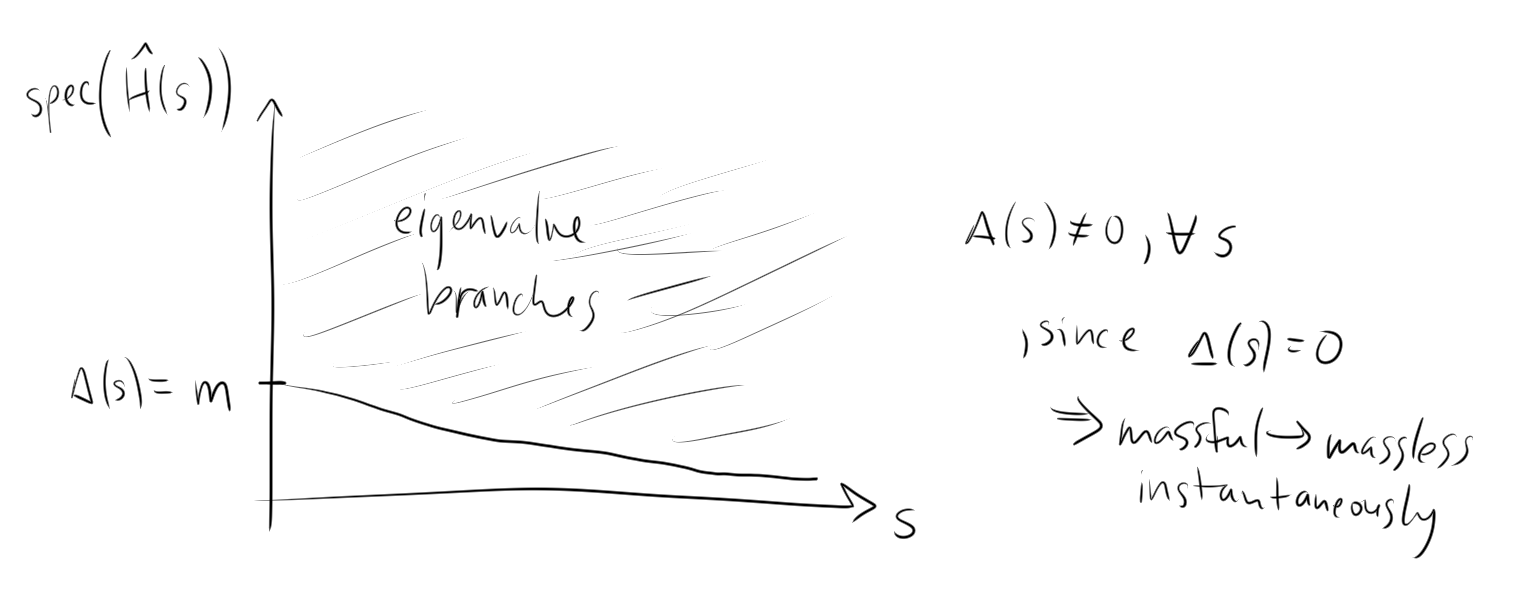
\includegraphics[scale=0.4]{images/eivs.png}
	\caption{Schematic of the spectral gap for the parameterized Hamiltonian.}
\end{figure}

\noindent For the proportionality factor of $\ket{k_A k_B}_{int}$ to be true for small interactions, which is far more radical, it is required that there are nonzero spectral gaps, for some $s>0$, at each momentum eigenstate of momenta $\textbf{k}_A$ and $\textbf{k}_B$, and there are no other nearby eigenvalues that may be mistaken for the incoming momenta. In practice, these incoming particles can create bound states, for example, and make this distinction difficult. If all of this is justifiable, and we accept the proportionality $\ket{k_A k_B}_{int} \propto \lim_{t\to\infty} e^{-i\hat{H}t} \ket{k_A k_B}_0$, then we can create equalities and proportionalities, although difficult, to quantities that we can actually calculate
\begin{equation}
\lim_{t\to\infty} \,_{0}\bra{\textbf{p}_1 \dots \textbf{p}_n} e^{-i hat{H} \cdot 2t} \ket{\textbf{k}_A \textbf{k}_B}_0 \propto \lim_{t\to\infty} \,_{0}\bra{\textbf{p}_1 \dots \textbf{p}_n} \mathcal{T}[ e^{-i \int^t_{-t} \hat{H}_{int}(t')dt'}] \ket{\textbf{k}_A \textbf{k}_B}_0
\end{equation}

\noindent This is exactly the same as the argument for the Dyson series expansion for $G^{(n)}$ with the vacuum states, and, just as in that case, the proportionality difficulty can be eliminated, and we have the following (not yet justified) equality
\begin{equation}
\bra{\textbf{p}_1 \dots \textbf{p}_n} i\hat{\mathbb{T}} \ket{\textbf{k}_A \textbf{k}_B} = \lim_{t\to\infty} \left( \,_{0}\bra{\textbf{p}_1 \dots \textbf{p}_n} \mathcal{T}[ e^{-i \int^t_{-t} \hat{H}_{int}(t')dt'}] \ket{\textbf{k}_A \textbf{k}_B}_0 \right)_{\tiny \stackanchor{connected,}{amputated}}
\end{equation}

\noindent The condition of "connected, amputated" is analogous to "connected" as in the $G^{(n)}$ case. \\

\noindent We can begin to justify this equality through some calculations. Consider the $\mathcal{O}(1)$ term, corresponding to the identity operator in  $\mathcal{S} = \mathbb{I} + i \hat{\mathbb{T}}$, for the $2\to 2$ scattering process.
\begin{align}
_{out}\braket{\textbf{p}_1 \textbf{p}_2 | \textbf{k}_A \textbf{k}_B}_{in} &=_{\mathcal{O}(1)} \,_{0}\braket{\textbf{p}_1 \textbf{p}_2 | \textbf{k}_A \textbf{k}_B}_{0} \\
&= \sqrt{2\omega_{p_1}\omega_{p_2}\cdot 2 \omega_{k_A}\omega_{k_B}} \bra{0} \hat{a}_{p_1} \hat{a}_{p_2} \hat{a}_{k_A}^\dagger \hat{a}_{k_B}^\dagger \ket{0} \\
&= 2\omega_A \cdot 2\omega_B (2\pi)^6 (\delta(\textbf{p}_1-\textbf{k}_A)\delta(\textbf{p}_2-\textbf{k}_B) + \delta(\textbf{p}_1-\textbf{k}_B)\delta(\textbf{p}_2-\textbf{k}_A))
\end{align}

\begin{figure}[H]
	\centering
	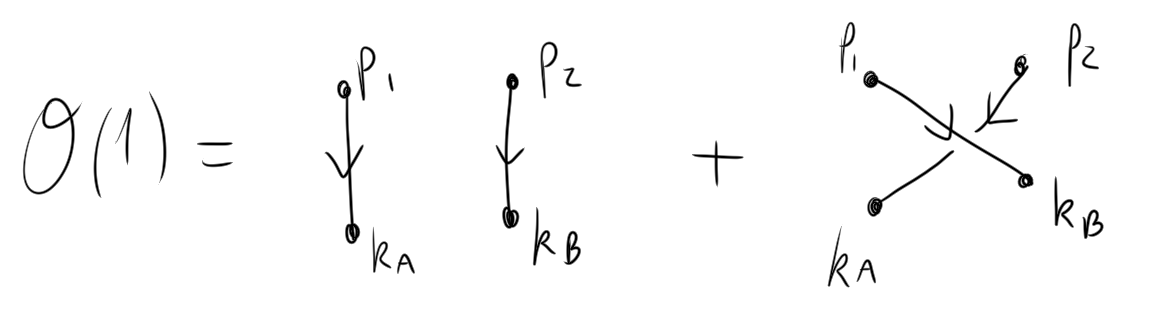
\includegraphics[scale=0.4]{images/o1.png}
	\caption{Diagram of the $\mathcal{O}(1)$ term as calculated above.}
\end{figure}

\noindent The next term to $\mathcal{O}(\lambda)$, applying Wick's theorem, and retaining all contractions, since we are not just working with the vacuum state anymore,
\begin{align}
\bra{\textbf{p}_1 \textbf{p}_2} i\hat{\mathbb{T}} \ket{\textbf{k}_A \textbf{k}_B}  &=_{\mathcal{O}(\lambda)} \,_{0}\bra{\textbf{p}_1 \textbf{p}_2} \mathcal{T}[ \frac{-i\lambda}{4!} \int d^4 x \, \hat{\phi}_I^4(\textbf{x}) ] \ket{\textbf{k}_A \textbf{k}_B}_{0} \\
&= \,_{0}\bra{\textbf{p}_1 \textbf{p}_2} \mathcal{N}[ \frac{-i\lambda}{4!} \int d^4 x \, \hat{\phi}_I^4(\textbf{x}) + {\tiny \stackanchor{all}{contractions}}\, ] \ket{\textbf{k}_A \textbf{k}_B}_{0}
\end{align}

\noindent To see what kinds of terms that survive to order $\lambda$, consider the interacting creation field operator interacting with the free four-momentum eigenstate
\begin{align}
\hat{\phi}_I^\dagger(\textbf{x}) \ket{\textbf{p}}_0 &= \int \frac{d^3 k}{(2\pi)^3} \, \frac{1}{\sqrt{2 \omega_k}} e^{-i \textbf{k}\cdot\textbf{x}} \hat{a}_k \ket{p} \\
&= \int \frac{d^3 k}{(2\pi)^3} \, \frac{1}{\sqrt{2 \omega_k}} e^{-i \textbf{k}\cdot\textbf{x}} \hat{a}_k \cdot \sqrt{2 \omega_p} \hat{a}_p^\dagger \ket{0} \\
&= \int \frac{d^3 k}{(2\pi)^3} \, \frac{1}{\sqrt{2 \omega_k}} e^{-i \textbf{k}\cdot\textbf{x}} \cdot (2\pi)^3 \delta^{(3)}(k-p) \sqrt{2\omega_p} \ket{0} \\
\hat{\phi}_I^\dagger(\textbf{x}) \ket{\textbf{p}}_0 &= e^{-i p\cdot x} \ket{0} .
\end{align}

\noindent To deal with momentum eigenstates, such as $\ket{\textbf{k}_A \textbf{k}_B}$, include them in \textit{extended contractions} by defining
\begin{align}
\wick[offset=1.5em]{\c {\hat{\phi}_I^\dagger(\textbf{x})} \c {\ket{p}} } &= e^{-i \textbf{p}\cdot \textbf{x}} \\
\wick[offset=1.5em]{\c {\bra{p}} \c {\hat{\phi}_I^\dagger(\textbf{x})}} &= e^{i \textbf{p}\cdot \textbf{x}}
\end{align}

\noindent Now, we can prove (\textbf{Exercise}) an extended version of Wick's theorem, where the time-ordered product of field operators in the presence of incoming and outgoing momentum eigenstates is equal to the sum over all possible contractions, including contractions of the field operators with the states as well.
\begin{equation}
_{0}\bra{\textbf{p}_1 \dots \textbf{p}_n} \mathcal{T}[{\small\text{field operators}}] \ket{\textbf{k}_1 \dots \textbf{k}_n} _{0} = \sum {\tiny \stackanchor{all possible full contractions}{including momentum eigenstates}}
\end{equation}

\noindent This allows us to approximate the $\mathcal{S}$-matrix transition amplitudes, justified up to the assumption about momentum eigenstates in the free theory being related to momentum eigenstates in the interacting theory.

\clearpage

\section{Lecture 13: Feynman Diagram Expansions in $\varphi^4$ Theory}
\label{sec:lec13}

\noindent In overview, thus far we have take a progression of reasonable, small steps to building a relativistic quantum field theory. We established Lorentz invariance as a symmetry of the theory, which may not quite be a fundamental symmetry of nature, but has not been violated by any experiments to date. Next, we established a unitary representation of the Poincar\'e group (difficult since the Poincar\'e group is not compact, unlike rotation groups), where space and time can transform into other via Lorentz boosts, meaning that energy and momentum can also exchange roles under Poincar\'e symmetries. This also causes difficulties in writing down quantum mechanical Hamiltonians that behave appropriately, but, fortunately, we can invoke locality in the theory, which is also seemingly fundamental to nature. Motivated by classical examples, such as the Klein-Gordon equation, a free theory, we write the relativistic quantum field theory, namely the quantum Klein-Gordon field, by "just putting hats" on the operators, and it worked. \\

\noindent To account for interactions, we added a perturbative $\varphi^4$ term to the quantum Klein-Gordon Hamiltonian
\begin{equation}
\hat{H}_{KG} \to \hat{H}_{KG} + \hat{H}_{\varphi^4}
\end{equation}

\noindent Where $\hat{H}_{\varphi^4}$ is Lorentz invariant, but is also an unbounded operator on any Hilbert space, such that $||\hat{H}_{\varphi^4} || \to \infty$. Though this is not mathematically rigorous, our forefathers and foremothers have shown through physical rigor, as well as time and time again by using tools outside of the realm of their mathematical applicability, that this is an acceptable perturbative term to account for field interactions. \\

\subsection*{Examples of Mathematically Non-Rigorous Applications}

\begin{itemize}
\item The building block of perturbation theory assumes that the interacting theory vacuum state is proportional to the free theory vacuum state via the time-evolution operator of the interacting theory
	\subitem $\ket{\Omega} \propto \lim_{t\to\infty} e^{-i\hat{H}_{\varphi^4}t} \ket{\Omega_0}$.
	\begin{itemize} 
	\item Even for finite dimensional systems, this limit does not exist and is oscillatory. The limit can make sense for Hamiltonians with a continuous spectra with a few particles.
	\end{itemize}
\item The momentum eigenstates require preparation of delta functions in the momenta, and are assumed to be related similar to the vacuum states
	\subitem $\ket{\textbf{p}_1 \dots \textbf{p}_n} = \lim_{t\to\infty} e^{-i\hat{H}_{\varphi^4}t} \ket{\textbf{p}_1 \dots \textbf{p}_n}_0$.
\item The Dyson series, a Taylor expansion of the interacting theory time evolution operator can not be expected to converge
	\subitem $e^{-i\hat{H}_{\varphi^4}t} = e^{-i\hat{H}_{KG}t} -i \int_0^t dt' \, e^{-i\hat{H}_{KG}t'} \hat{H}_I e^{i\hat{H}_{KG}t'} + \dots$.
\end{itemize}

\noindent We are often punished by infinities, where we would prefer finite numbers. Some infinities are trivially removable with no operational consequence, such as the ground state energy shift in the Klein-Gordon theory, such that $E_0 \to E_0 + \infty$ . Other infinities can be factored away by rescaling observables, such as in the case of vacuum bubbles (e.g., $\frac{\infty}{\infty} = 1$). Yet other infinities just don't go away, such as in the diagram of two internal vertices. \\

\noindent Perhaps the choice of interaction terms is the cause of all of these infinities, and we can impose a cutoff to the theory that will eliminate some infinities. For example, in the $\varphi^4$ theory
\begin{equation}
\hat{H}_{\varphi^4} \to \hat{H}_{\varphi^4}(\Lambda)
\end{equation}

\noindent Where $\Lambda$ is a cutoff up to some family of models/theories, and the norm of the cutoff Hamiltonian is proportional to the cutoff, which may be large, but not infinity, such that $||\hat{H}_{\varphi^4}(\Lambda) || \propto \Lambda$. \\

\noindent For example, consider the quantum harmonic oscillator cutoff, where $||\hat{H}(N)|| = N$
\begin{equation}
\hat{H} = \sum_{n=0}^{\infty} (n+\frac{1}{2}) \ket{n}\bra{n} \to \hat{H}(N) = \sum_{n=0}^N (n+\frac{1}{2}) \ket{n}\bra{n} + \sum_{n>N} (N+\frac{1}{2}) \ket{n}\bra{n}
\end{equation}

\noindent The major concern with imposing cutoffs is whether observables depend on the cutoff or not. To eschew this issue, we allow unobservable parameters, coupling constants, to shift and absorb all the cutoff dependence. \\

\subsection*{Renormalization}

\noindent This practice is called \textbf{renormalization}, and it works. We make the hypothesis that the Hamiltonian depends on some number of parameters, called coupling constants, such that $\hat{H} = \hat{H}(z_1,\dots,z_n)$. The mapping from the coupling constants to observables is not expected to be, and is usually not, bijective. For example,
\begin{equation}
\hat{H}_{\varphi^4}(\lambda, m) = \int d^3 x \, \left( \nabla^2 \hat{\phi} + m^2 \hat{\phi}^2 + \frac{\lambda}{4!} \hat{\phi}^4 \right)
\end{equation}

\noindent This Hamiltonian corresponds to a list of observables $\mathcal{O}_j(z_1,\dots, z_n)$, $j=1,2,\dots$, with complicated (nonlinear) dependencies with the coupling constants, which usuaslly exist on a smooth manifold before mapping to observables. \\

\noindent For example, consider the spectral gap $\mathcal{O} = E_1-E_0$, where $\mathcal{O} = \mathcal{O}(z_1+c,z_2,\dots,z_n)$, and $\hat{H} = z_1\cdot \mathbb{I} + \hat{H}'(z_2,\dots,z_n)$. \\

\noindent Add the cutoff dependence to the observables, such that 
\begin{equation}
\hat{H}_\Lambda (z_1,\dots, z_n) \to \mathcal{O}_{expt.} = \mathcal{O}_j(z_1,\dots,z_n;\Lambda)
\end{equation}

\noindent If "lucky", each of the coupling constants can absorb all of the $\Lambda$-dependence, and none of the observables will depend directly on the cutoff
\begin{equation}
\mathcal{O}_{expt.} = \mathcal{O}_j(z_1,\dots,z_n;\Lambda) = \mathcal{O}_j(z_1(\Lambda) , \dots , z_n(\Lambda)) .
\end{equation}

\noindent If the above is true, then the theory is renormalizable, and is now defined by a highly overdetermined set of equations, such that there are a finite number of parameters $z_i$ and an infinite list of equations (observables) $\mathcal{O}_j$ to solve. Renormalizable theories effectively have no cutoff, since the remaining infinities are eliminated by changing the order of limits.
\begin{enumerate}
\item Take the limit as the cutoff tends to infinity, $\Lambda \to \infty$, then compute observable quantities.
\item Vice versa.
\end{enumerate}

\subsection*{Typical Terms in Scattering Experiments}

\noindent Scattering experiments generate interaction terms such as the following
\begin{equation}
\,_0 \bra{p_1 p_2 \dots p_n} \mathcal{T} \, [\frac{\lambda}{4!} \int d^4 x \, \hat{\phi}_I^4(x)]\ket{q_A q_B}_0 \,.
\end{equation}

\noindent Apply (generalized) Wick's theorem to calculate the contractions, and sum over three types of terms (to order $\lambda$) encountered. Note that $\hat{\phi}_I (x) = \hat{\phi}$ in the following. Wick's theorem applied to $\mathcal{T}[\hat{\phi}^4 (x)]$ yields a sum over the normal ordering of all of the following contractions, such that 
\begin{equation}
\mathcal{T}[\hat{\phi}^4 (x)] = \text{fully contracted} + \text{partially contracted} + \text{uncontracted}
\end{equation}
\begin{align*}
\textbf{Fully contracted}: &\,\,\,\, \mathcal{N}[ \wick[offset=1.2em]{\c1 {\hat{\phi}} \c1 {\hat{\phi}} \c2 {\hat{\phi}} \c2 {\hat{\phi}} }] + \text{other fully contracted} \\
\textbf{Partially contracted}: &\,\,\,\, \mathcal{N}[ \wick[offset=1.2em]{\c {\hat{\phi}} \c {\hat{\phi}} {\hat{\phi}} {\hat{\phi}}} + \wick[offset=1.2em]{\c {\hat{\phi}} {\hat{\phi}} \c {\hat{\phi}} {\hat{\phi}}}] + \text{other partially contracted} \\
\textbf{Uncontracted}: &\,\,\,\, \mathcal{N} [ \hat{\phi} \hat{\phi} \hat{\phi} \hat{\phi}].
\end{align*}

\noindent The diagrammatic contributions to the integrals from each type of contracted term to the $\mathcal{S}$-matrix have the following forms (for the $n=2$ case) \\

\noindent \textbf{Type 1, fully contracted:} 

\begin{equation}
\frac{-i\lambda}{4!} \int d^4 x \,_0 \bra{p_1 p_2} \wick[offset=1.2em]{\c1 {\hat{\phi}} \c1 {\hat{\phi}} \c2 {\hat{\phi}} \c2 {\hat{\phi}} } \ket{q_A q_B}_0 =
\end{equation}
\begin{figure}[H]
	\centering
	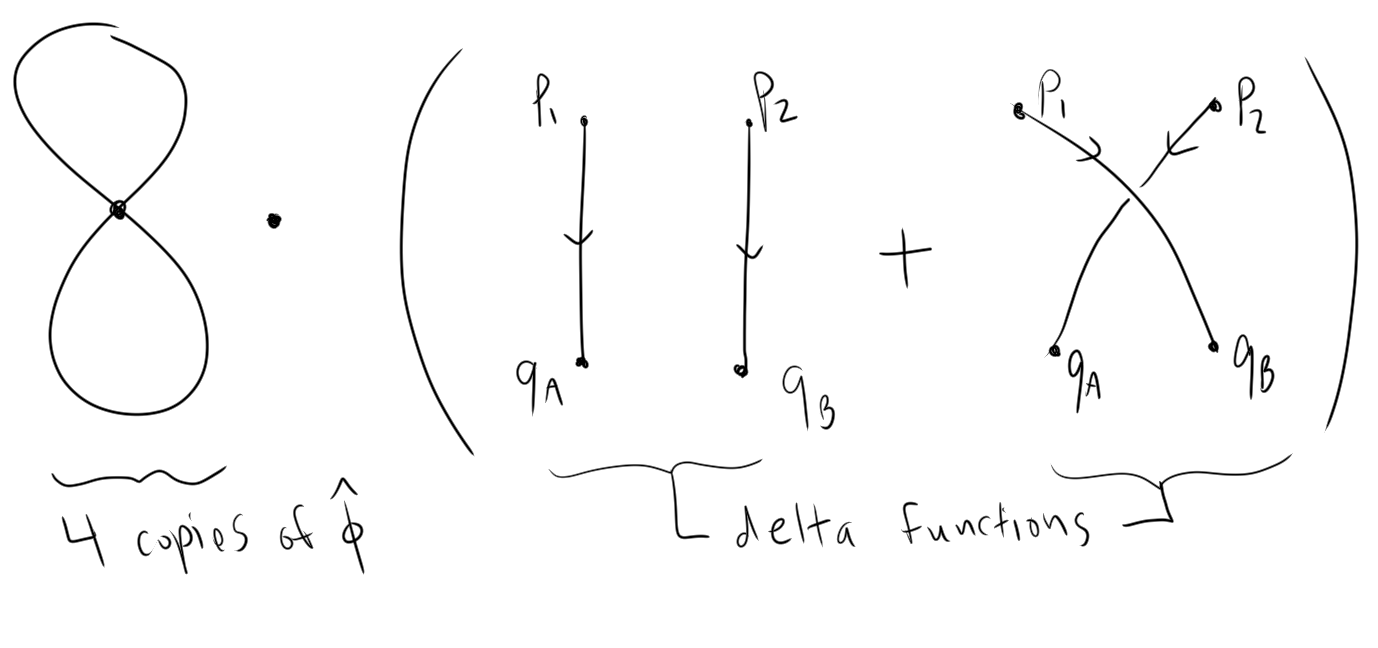
\includegraphics[scale=0.4]{images/fullcont.png}
	\caption{Diagrammatic contributions of fully contracted terms: a product of fully connected diagrams, from four copies of the field operator (figure eight), and delta functions imposing a sort of momentum conservation.}
\end{figure}

\noindent The full contraction is just a $\mathbb{C}$ number, making the integral over the inner product of momentum eigenstates. \\

\noindent \textbf{Type 2, partially contracted:}

\begin{equation}
\frac{-i\lambda}{4!} \int d^4 x \,\,_0\bra{p_1 p_2} \wick[offset=1.2em]{\c {\hat{\phi}} \c {\hat{\phi}}} \,\mathcal{N}[\hat{\phi} \hat{\phi}] \ket{q_A q_B}_0 = \frac{-i\lambda}{4!} \int d^4 x \, ( \, (1) + (2) + (3) \, )
\end{equation}

\noindent The partial contractions have three more types of normal orderings, as labelled above: $(1) + (2) + (3)$
\begin{enumerate}
\item \textbf{Right:} $\wick[offset=1.5em]{\c {\hat{\phi}} \c {\hat{\phi}}} \,\,_0\bra{p_1 p_2} \wick[offset=1.5em]{\c1 {\hat{\phi}} \c2 {\hat{\phi}} \ket{ \c1 {q_A} \c2{q_B} }_0 } + $ all other contractions to the right.
\item \textbf{Left:} $\wick[offset=1.5em]{\c {\hat{\phi}} \c {\hat{\phi}}} \, \wick[offset=1.5em]{ \,_0\bra{ \c1 {p_1} \c2 {p_2} } \c2 {\hat{\phi}} \c1 {\hat{\phi}}} \ket{q_A q_B}_0  + $ all other contractions to the left.
\item \textbf{Both:} $\wick[offset=1.5em]{\c {\hat{\phi}} \c {\hat{\phi}}} \, \wick[offset=1.5em]{ \,_0\bra{ \c1 {p_1} p_2} \c1 {\hat{\phi}} \c2 {\hat{\phi}} \ket{ \c2 {q_A} q_B }_0 } + $ all other contractions one left and one right.
\end{enumerate}

\begin{figure}[H]
	\centering
	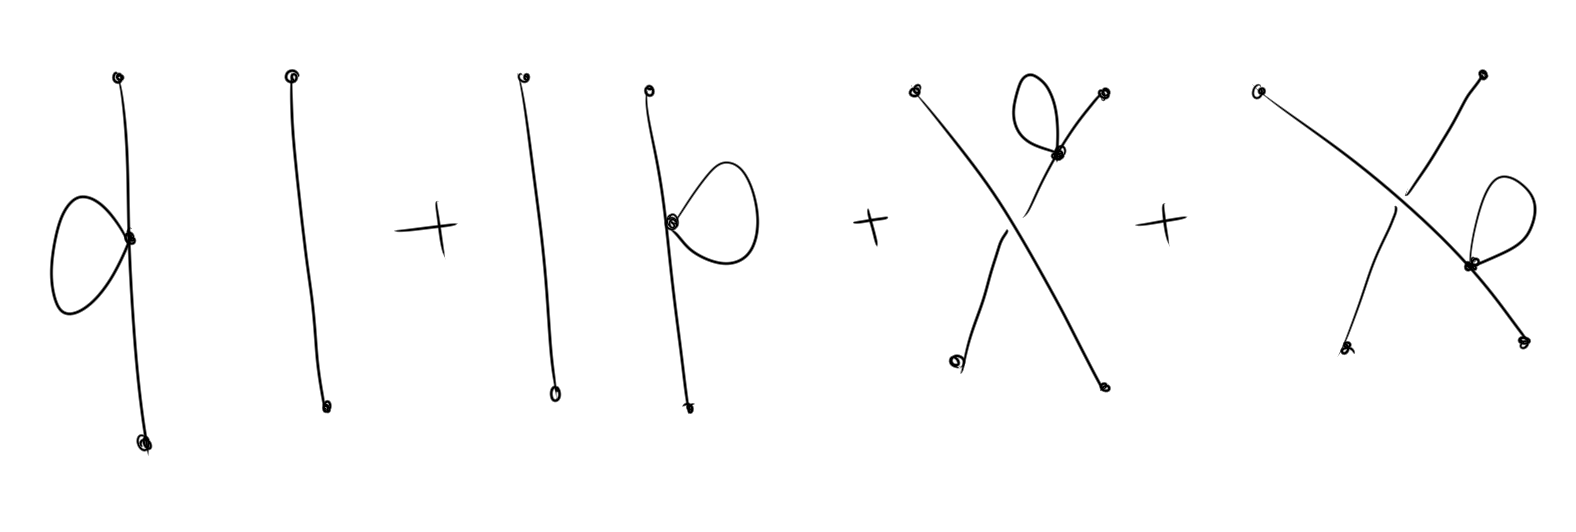
\includegraphics[scale=0.4]{images/partcont.png}
	\caption{Diagrammatic contributions of partially contracted terms.}
\end{figure}

\noindent Note that the contraction of the interacting field operators and the momentum eigenstates, as in the three cases above, contribute incoming/outgoing momenta, a vertex, and three external legs.

\begin{figure}[H]
	\centering
	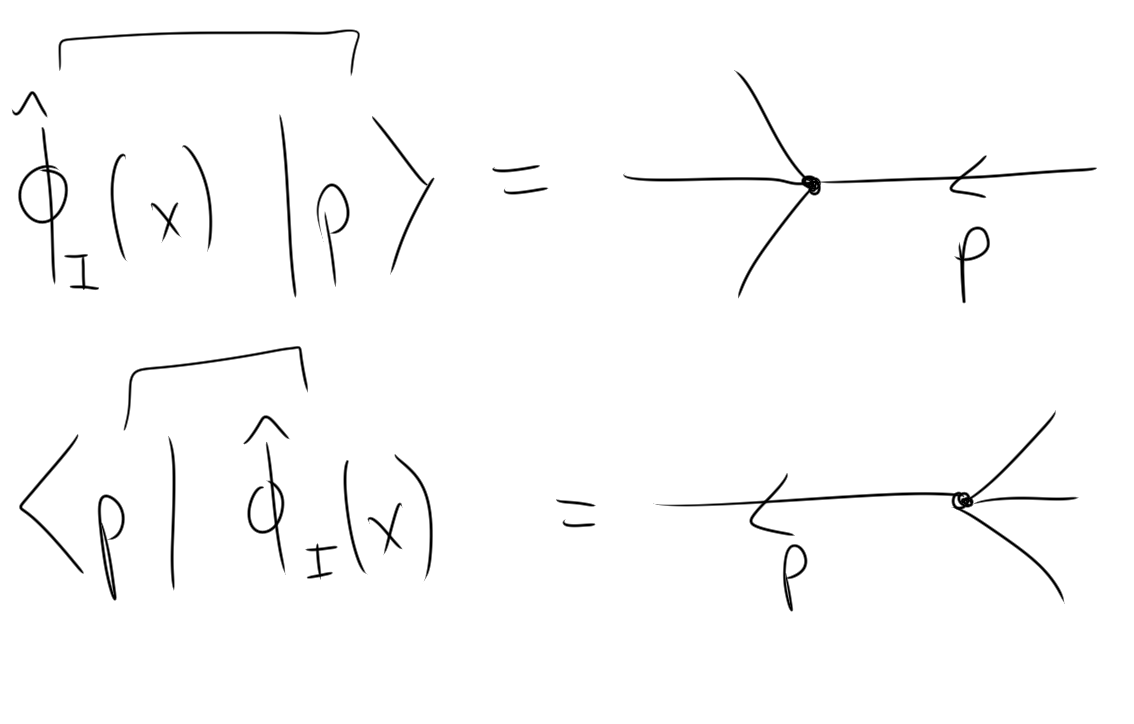
\includegraphics[scale=0.3]{images/opstatecont.png}
	\caption{Diagrammatic contributions of contractions between intertacting field operators and momentum eigenstates.}
\end{figure}

\noindent \textbf{Type 3, uncontracted:} 

\begin{align*}
\frac{-i\lambda}{4!} \int d^4 x \,\,_0\bra{p_1 p_2} \mathcal{N}[\hat{\phi} \hat{\phi} \hat{\phi} \hat{\phi}] \ket{q_A q_B}_0 &= \, \frac{-i\lambda}{4!} \cdot 4! \cdot \int d^4 x e^{-i(q_A + q_B - p_1 - p_2) \cdot x} \\
&= -i \lambda (2 \pi)^4 \delta^{(4)} (q_A + q_B - p_1 - p_2) \\
&= \text{Diagram below.}
\end{align*}

\begin{figure}[H]
	\centering
	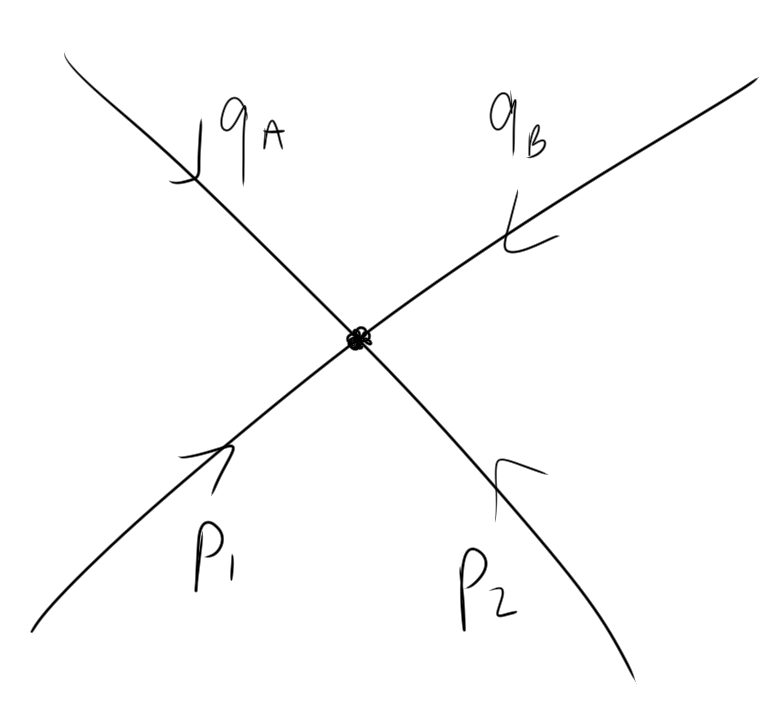
\includegraphics[scale=0.3]{images/momcons.png}
	\caption{Uncontracted term contributes diagram that enforces momentum conservation.}
\end{figure}

\noindent Adding all of the terms together in the full expansion of the interacting component of the $\mathcal{S}$-matrix, namely $\,_0\bra{p_1 p_2} i\hat{\mathbb{T}} \ket{q_A q_B}_0$, we get a series lke the following

\begin{figure}[H]
	\centering
	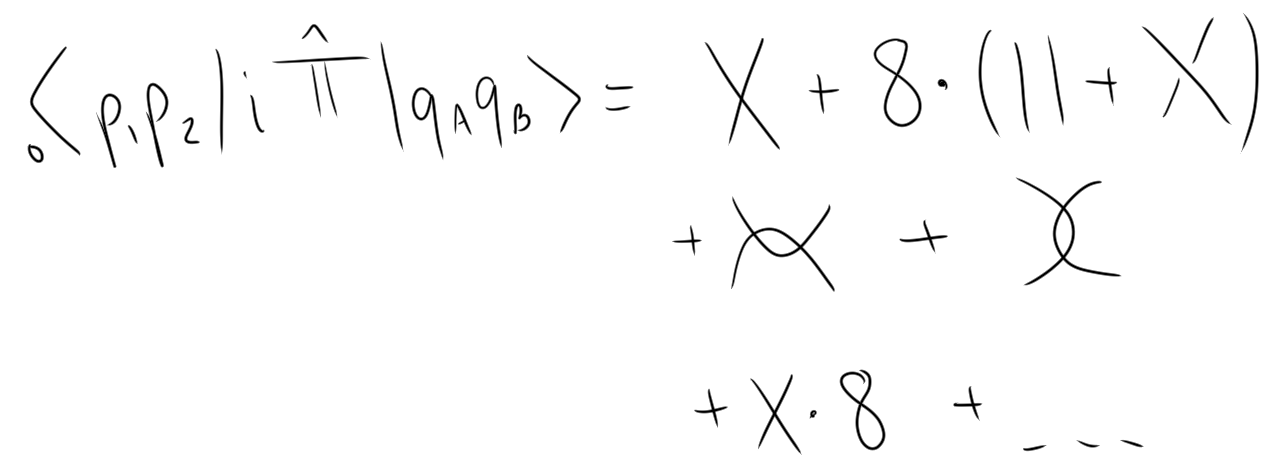
\includegraphics[scale=0.4]{images/tmatrix.png}
	\caption{Full diagrammatic expansion of the interacting component fo the $\mathcal{S}$-matrix.}
\end{figure}

\noindent These are the three types of diagrams, with respect to connectedness, that are always encountered: fully connected, partially connected, and vacuum bubble times cully connected.

\begin{figure}[H]
	\centering
	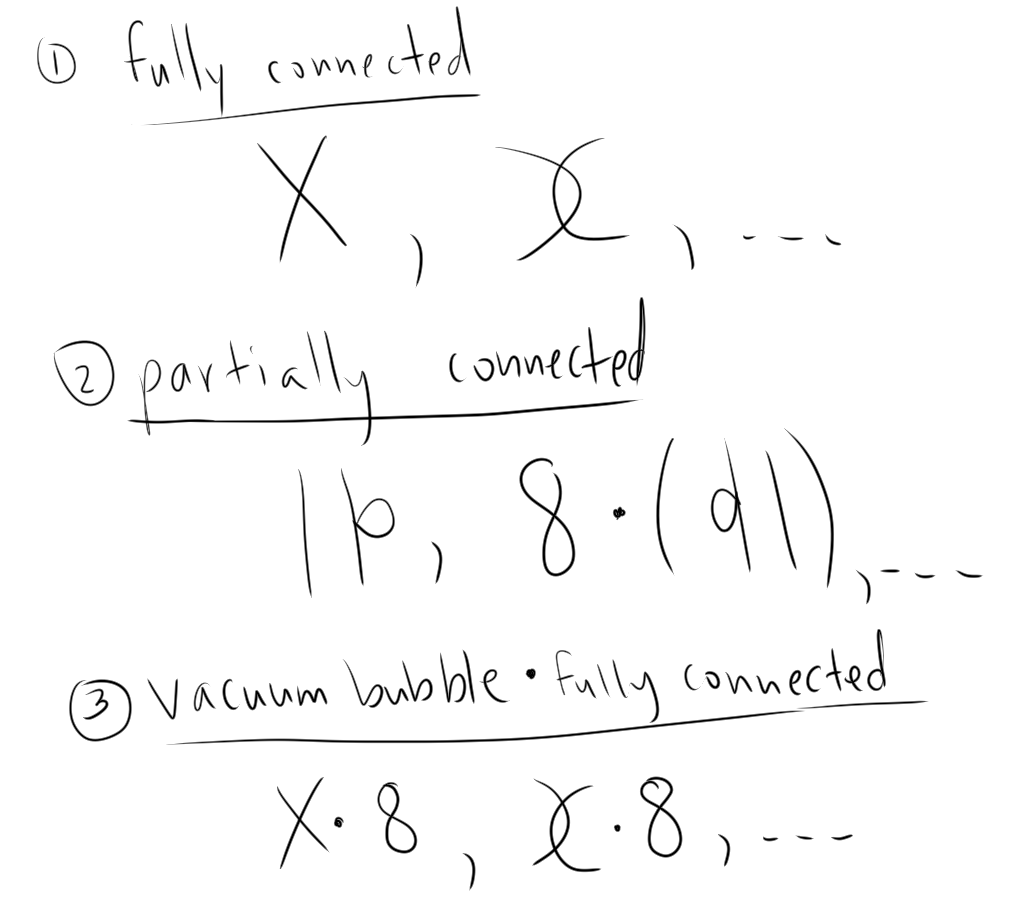
\includegraphics[scale=0.6]{images/connectiontypes.png}
	\caption{Three types of connectedness encountered in diagrammatic expansions of the interacting component of the $\mathcal{S}$-matrix.}
\end{figure}
 
\subsection*{Vacuum Bubbles and Fully Connected Diagrams}

\noindent Claim, here without proof, that products of vacuum bubbles and fully connected diagrams exponentiate, and, further, the only diagrams which contribute to the $\mathcal{S}$-matrix are the fully connected diagrams. There still exist fully connected diagrams (integrals) that result in infinities. To quell these infinities, either impose a cutoff scale, \textbf{or} argue that such a diagram does not contribute to the $\mathcal{S}$-matrix. \\

\begin{figure}[H]
	\centering
	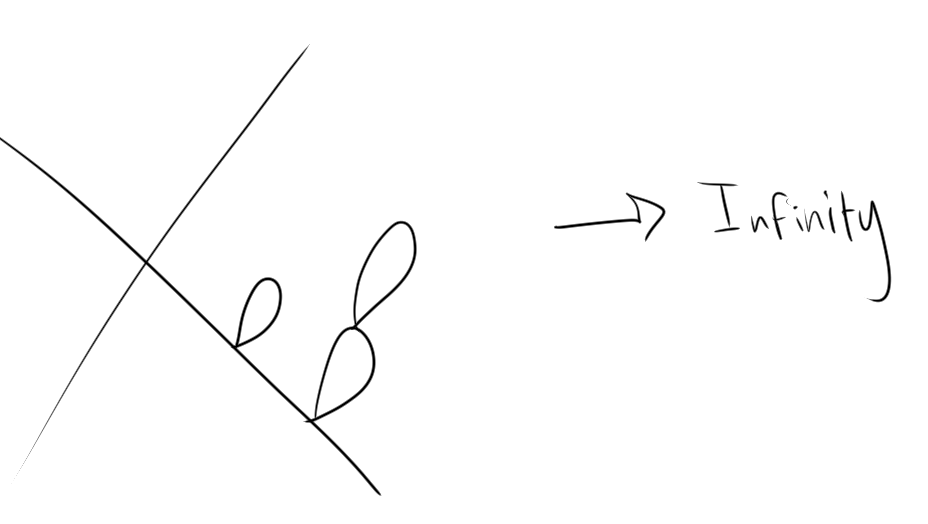
\includegraphics[scale=0.4]{images/fullconninf.png}
	\caption{An example of a fully connected diagram that results in infinity.}
\end{figure}

\noindent \textbf{External leg corrections} may be used to "amputate" parts of a diagram that will remove infinities from the external legs. This process represents a projection from the free momentum eigenstates to the interacting momentum eigenstates, just as in the projection of the vacuum state $\ket{\Omega}$. Thus, external leg corrections factorize the diagram. 
\begin{equation}
\ket{q_B}_0 \to \ket{q_B}
\end{equation}

\begin{figure}[H]
	\centering
	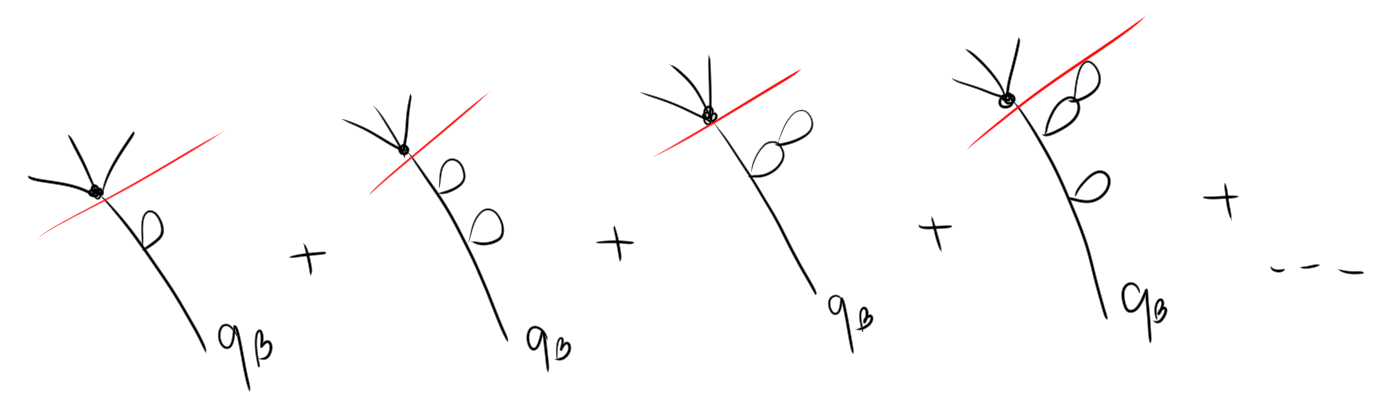
\includegraphics[scale=0.4]{images/extlegcorr.png}
	\caption{Single cuts made from the body of the diagram are called \textit{external leg corrections}, and "amputate" off infinities.}
\end{figure}

\noindent Amputation can not remove all infinities, since it is defined via the external leg corrections. Self-interactions on internal legs are not removable via amputation.

\begin{figure}[H]
	\centering
	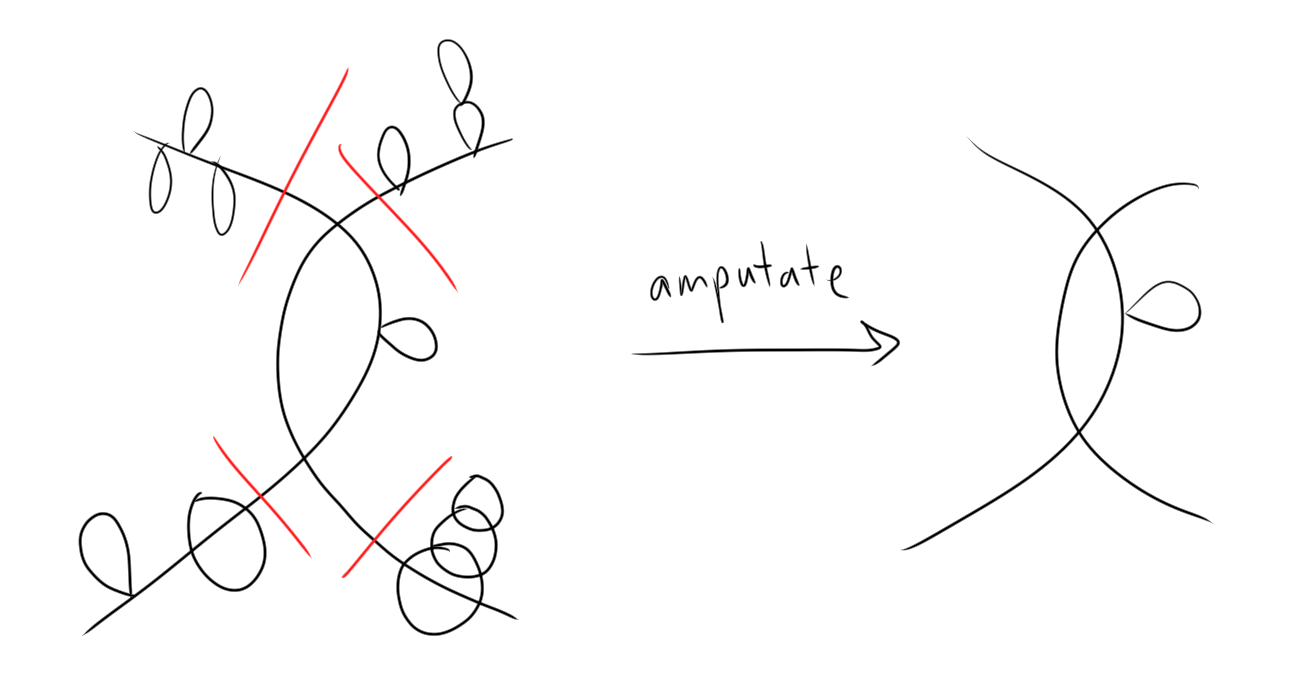
\includegraphics[scale=0.4]{images/amputation.png}
	\caption{An example of an amputation process where not all infinities can be removed, since it is not on an external leg.}
\end{figure}

\noindent And the final statement of the Feynman rule for the $\varphi^4$ interaction theory reads

\begin{equation}
i \mathcal{M} (2\pi)^4 \delta^{(4)} (q_A + q_B - \sum_f p_f) = \left( \stackanchor{\stackanchor{sum of all connected and}{amputated Feynamn diagrams}}{\stackanchor{with incoming momenta $q_A$, $q_B$}{and outgoing momenta $p_f$}} \right)
\end{equation} 

\clearpage

\section{Lecture 14: The Dirac Field}
\label{sec:lec14}


\noindent We've built a relativistic quantum field theory for the (complex) scalar field, or spinless particles, around the Klein-Gordon equation and its Lorentz group invariant, conserved quantities, or the generators of Lorentz transformations (e.g., boosts and rotations), which obey the Lie algebra bracket

\begin{equation}
[J^{\rho \sigma}, J^{\tau \nu}] = \eta^{\sigma \tau} J^{\rho\nu} - \eta^{\rho \tau} J^{\sigma \nu} + \eta^{\rho\nu} J^{\sigma \tau} - \eta^{\sigma \nu} J^{\rho \tau} .
\end{equation} 

\noindent We now build a relativistic quantum field theory for fermions, particles of spin-$\frac{1}{2}$, which requires a (complex) vector, or spinor, field to describe the dynamics of the fermionic field. Our strategy is similar to the scalar field case:

\begin{itemize}
\item Build a relativistic classical field theory.
\item Quantize the field (by guess).
\item Check for the (projective) representation of the Lorentz group.
\end{itemize}

\noindent To begin with building the relativistic classical field theory, given a set of objects obeying the Lie bracket above, we construct a Lagrangian by first constructing the representation of the Lorentz group via $g=e^{-\frac{i}{2} \omega_{\mu\nu}J^{\mu\nu}}$, where $\omega_{\mu\nu}$ are the Lorentz boost parameters, and then calculating Lagrangian densities invariant under the representation $g$.

\subsection*{Dirac's Motivation}

\noindent Dirac desired to factorize the Klein-Gordon equation, and craft an equation of motion linear in spacetime derivatives $\partial_\mu \equiv \partial / \partial x^\mu$, the square root of the Klein-Gordon equation, such that any solution to the Dirac equation is also a solution to the Klein-Gordon equation, but not necessarily vice versa. Linearity in the spacetime derivatives ensures that the associated probability current is positive definite, and the positive energy solutions may be separated from the negative energy solutions inherent to solutions of the Klein-Gordon equation. \\

\noindent The Dirac equation, which we will motivate and derive, reads

\begin{equation}
(i \gamma^\mu \partial_\mu - m) \psi = 0 .
\end{equation}

\noindent Where the coefficients of the spacetime derivatives $i\gamma^\mu$ can not be just four scalar quantities, as the vector of coefficients would then define a direction, and the Dirac equation would not be Lorentz invariant. The $\gamma^\mu$ must actually be $4\times 4$ matrices, and the field $\psi$ must be a four-vector. \\

\noindent To recover the Klein-Gordon equation from the Dirac equation, multiply the Dirac equation by $(i \gamma^\nu \partial_\nu + m)$, and compare to the Klein-Gordon equation $(\partial^2 + m^2)\psi=0$ to see that the "squared" Dirac equation becomes the Klein-Gordon equation if the \textit{gamma matrices} obey the following anticommutation relation

\begin{equation}
\{ \gamma^\mu, \gamma^\nu \} = 2 \eta^{\mu\nu} \cdot \mathbb{I}_{n \times n}.
\end{equation}

\noindent Where $\eta^{\mu\nu}$ is the Minkowski metric tensor.

\subsection*{Generators of Fermionic Field (Lorentz) Transformations}

\noindent To calculate the generators of the Lorentz transformations of the fermionic field (spin-$\frac{1}{2}$ particles), suppose that we have that set of 4 $n \times n$ matrices $\gamma^\mu$ that satisfy the anticommutation relation $\{ \gamma^\mu, \gamma^\nu \} = 2 \eta^{\mu\nu} \cdot \mathbb{I}_{n \times n}$. Obtain a solution in terms of the gamma matrices that obeys the Lie algebra bracket above

\begin{equation}
J^{\mu\nu} \to S^{\mu\nu} \equiv \frac{i}{4} [\gamma^\mu, \gamma^\nu].
\end{equation}

\noindent It is an \textbf{(exercise)} to check that these generators obey Lie algebra bracket above for the Lorentz transformation, and that four dimensions is the minimum of the gamma matrices dimensionality for nontrivial solutions. \\

\noindent The gamma matrices that correctly form the Lorentz group in $(3+1)$d spacetime were crafted by Dirac via the Pauli spin (sigma) matrices

\begin{equation}
\gamma^0 = \left( \begin{array}{c|c} 0 & \mathbb{I} \\ \hline \mathbb{I} & 0 \end{array} \right) \,\,\,\,\,\,\,\, \gamma^j = \left( \begin{array}{c|c} 0 & \sigma^j \\ \hline -\sigma^j & 0 \end{array} \right) .
\end{equation}

\noindent Where the Pauli sigma matrices read
\begin{equation}
\sigma^1 = \left( \begin{array}{cc} 0 & 1 \\ 1 & 0 \end{array} \right) \,\,\,\, \sigma^2 = \left( \begin{array}{cc} 0 & -i \\ i & 0 \end{array} \right) \,\,\,\, \sigma^3 = \left( \begin{array}{cc} 1 & 0 \\ 0 & -1 \end{array} \right) .
\end{equation}

\noindent The timelike components $S^{0j}$ yield three ($j=1,2,3$) boost generators of the Lorentz group (of the Lie algebra above)
\begin{equation}
S^{0j} = \frac{i}{4} \left[ \gamma^0, \gamma^j \right] = -\frac{i}{2} \left(\begin{array}{cc} \sigma^j & 0 \\ 0 & -\sigma^j \end{array} \right) .
\end{equation}

\noindent The other six generators from the spacelike components have the form
\begin{equation}
S^{jk} = \frac{i}{4} \left[ \gamma^j, \gamma^k \right] = \frac{1}{2} \epsilon^{jkl} \left(\begin{array}{cc} \sigma^l & 0 \\ 0 & -\sigma^l \end{array} \right)
\end{equation}

\noindent Where the sigma matrices obey the commutation relation: $[\sigma^j,\sigma^k] = 2i\epsilon^{jkl} \sigma^l$. \\

\subsection*{Construction of Gamma Matrices}

\noindent To build the operators that obey the desired anticommutation relation, and also form a \textit{Clifford algebra}, implement the \textbf{Jordan-Wigner transformation}, which maps the Pauli sigma matrices to fermionic creation and annihilation operators.

\subsubsection*{Jordan-Wigner Transformation}

\noindent Suppose that you want to represent operators that obey the (fermionic) anticommutation relation
\begin{equation}
\{\mu^a, (\mu^b)^\dagger\} = \delta^{ab}, \,\,\,\, a,b \, = \, 1,2,\dots,n.
\end{equation}

\noindent Consider the operator $\sigma^+ = \left(\begin{array}{cc} 0 & 0 \\ 1 & 0 \end{array} \right)$, and the construction of successive operators which all operate on the same $n$-dimensional space, permissing the expanse of $n$ direct products with the unit operator
\begin{align*}
\mu^1 &= \sigma^+ \otimes \mathbb{I} \otimes \mathbb{I} \otimes \mathbb{I} \otimes \mathbb{I} \otimes \dots \otimes \mathbb{I} \\
\mu^2 &= \sigma^3 \otimes \sigma^+ \otimes \mathbb{I} \otimes \mathbb{I} \otimes \mathbb{I} \otimes \dots \otimes \mathbb{I} \\
\mu^3 &= \sigma^3 \otimes \sigma^3 \otimes \sigma^+ \otimes \mathbb{I} \otimes \mathbb{I} \otimes \dots \otimes \mathbb{I} \\
\mu^4 &= etc. \, \dots
\end{align*}

\noindent These $\mu^j$ operators obey the fermioic anticommutation relations, since $\{\sigma^j, \sigma^k \} = 2 \delta^{jk}$, and form a matrix representation of the anticommutation relation given in the Jordan-Wigner transformation.

\noindent An inefficient method to construct a representation of the gamma matrices, though reducible to the above $\mu^j$ matrices, which honors the anticommutation relation, starts with the composition of the timelike gamma matrix
\begin{equation}
\gamma^0 = \sigma^1 \otimes \mathbb{I} .
\end{equation}

\noindent Next, we know that $\sigma^2$ anticommutes with $\sigma^1$ via $\{\sigma^j, \sigma^k \} = 2 \delta^{jk}$, and thus we construct the following, noting that to satisfy $(\gamma^j)^2 <0$, scalar multiplication by the imaginary unit $i$ is required
\begin{equation}
\gamma^j \equiv i \sigma^2 \otimes \sigma^j .
\end{equation}

\subsection*{The Dirac Spinor}

\noindent The set of matrices $\gamma^\mu$ satisfying the anticommutation relation $\{ \gamma^\mu, \gamma^\nu \} = 2 \eta^{\mu\nu} \cdot \mathbb{I}_{n \times n}$ are called the \textbf{Dirac matrices}, and the four-component object that transforms correctly under the Lorentz group is called the \textbf{Dirac spinor}
\begin{equation}
\psi \to e^{-\frac{i}{2} \omega_{\mu\nu} S^{\mu\nu}} \psi
\end{equation}
This is the definition of the spinor in different reference frames, and defines the \textbf{spinor field} as a mapping
\begin{equation}
\psi: \mathbb{R}^{1,3} \to \mathbb{C}^4.
\end{equation}

\noindent Transforming as
\begin{equation}
\psi_a(x) = \sum_{b=0}^3 [ \Lambda_{1/2} ]_{ab} \,\, \psi_b(\Lambda^{-1}x), \,\, \Lambda \in SO(3)
\end{equation}

\noindent Where $\Lambda$ is the usual representation for the Lorentz transformation, and $\Lambda_{1/2}$ has the same representation structure and obeys the same Lie algebra of the Lorentz transformation, but different elements: the $4\times4$ matrix Lie algebra bracket $S^{\mu\nu}$ built out of the gamma matrices
\begin{align}
\Lambda &= e^{-\frac{i}{2} \omega_{\mu\nu} J^{\mu\nu}} \\
\Lambda_{1/2} &= e^{-\frac{i}{2} \omega_{\mu\nu} S^{\mu\nu}}
\end{align}

\noindent Every representation of the Lorentz group can be used to build Lorentz invariant field equations, such that $\mathcal{D}\psi=0$. To build the field equations for $\psi_a(x)$, first guess and check (\textbf{Exercise}) that the Klein-Gordon equation is satisfied
\begin{equation}
(\partial^2 + m^2) \psi_a(x) = 0, \, \forall \, a
\end{equation}

\noindent The next guess, by Dirac, is to find a satisfactory field equation that is linear in spacetime derivatives. This requires the following identity as an auxiliary computation between the gamma matrices and the two generators, first confirmed by Dirac (\textbf{Exercise})
\begin{equation}
[\gamma^\mu, S^{\rho\sigma}] = (J^{\rho\sigma})^\mu_{\,\,\,\nu} \, \gamma^\nu
\end{equation}

\noindent This is reminiscient of how the four-vector transforms under the Lorentz transformation, and we motivatedly write, to first order in $\omega$
\begin{align}
(1+\frac{i}{2}  \omega_{\rho\sigma} S^{\rho\sigma}) \gamma^\mu (1-\frac{i}{2}  \omega_{\rho\sigma} S^{\rho\sigma}) &= (1-\frac{i}{2}  \omega_{\rho\sigma} J^{\rho\sigma})^\mu_{\,\,\,\nu} \gamma^\nu \\
e^{\frac{i}{2} \omega_{\rho\sigma} S^{\rho\sigma}} \gamma^\mu e^{-\frac{i}{2} \omega_{\rho\sigma} S^{\rho\sigma}} &\approx (e^{-\frac{i}{2} \omega_{\rho\sigma} J^{\rho\sigma}})^\mu_{\,\,\,\nu} \gamma^\nu  \\
\Lambda_{1/2}^{-1} \gamma^\mu \Lambda_{1/2} &= \Lambda^\mu_{\,\,\,\nu} \gamma^\nu
\end{align}

\noindent This shows that the gamma matrices transform exactly like a four-vector under the Lorentz transformation. Contracted against another vector, that transforms accordinngly, will produce another Lorentz invariant object. The differential operator $\partial_\mu$ transforms as such, making $\gamma^\mu \partial_\mu$ Lorentz invariant. \\

\noindent Thus, the Lorentz invariant field equation, the Dirac equation, reads
\begin{equation}
(i\gamma^\mu \partial_\mu - m) \psi = 0
\end{equation}

\noindent Check the invariance of the Dirac equation by substituting the following quantities for the spinor and spacetime derivative into the Dirac equation (\textbf{Exercise})
\begin{align}
\psi(x) &\to \Lambda_{1/2} \psi \, (\Lambda^{-1}x) \\
\partial_\mu &\to (\Lambda^{-1})^\nu_{\,\,\,\mu} \partial_\nu .
\end{align}

\noindent Making these subsitutions, the Dirac equation becomes
\begin{align}
\left( i\gamma^\mu (\Lambda^{-1})^\nu_{\,\,\,\mu}\partial_\nu - m \right) \Lambda_{1/2}\, \psi(\Lambda^{-1}x) &= 0 \\
\Lambda_{1/2} \Lambda^{-1}_{1/2}\cdot \left( i\gamma^\mu (\Lambda^{-1})^\nu_{\,\,\,\mu}\partial_\nu - m \right) \Lambda_{1/2}\, \psi(\Lambda^{-1}x) &= 0 \\
\Lambda_{1/2}\, \left( i\Lambda^{-1}_{1/2}\,\gamma^\mu \Lambda_{1/2} \,(\Lambda^{-1})^\nu_{\,\,\,\mu}\partial_\nu - m \right) \psi(\Lambda^{-1}x) &= 0 \\
\Lambda_{1/2}\, \left( i\Lambda^\mu_{\,\,\,\sigma} \gamma^\sigma (\Lambda^{-1})^\nu_{\,\,\,\mu}\partial_\nu - m \right) \psi(\Lambda^{-1}x) &= 0 \\
\Lambda_{1/2}\, \left( i\gamma^\nu \partial_\nu - m \right) \psi(\Lambda^{-1}x) &= 0 
\end{align}

\noindent Going from line 2 to 3 utilizes the fact that $(\Lambda^{-1})^\nu_{\,\,\,\mu}\partial_\nu$ is a linear operator, meaning the quantity $\Lambda^{-1}_{1/2}\,\gamma^\mu \Lambda_{1/2}$ also transforms like a four-vector and is Lorentz invariant. Going from line 4 to 5 uses the fact that $(\Lambda^{-1})^\nu_{\,\,\,\mu}\partial_\nu \, \psi(\Lambda^{-1} x)$ is a delta function. The left hand side becomes zero, and the Dirac equation is Lorentz invariant. \\

\noindent The Dirac equation contains the Klein-Gordon equation
\begin{align*}
(i\gamma^\mu \partial_\mu - m) \psi &= 0 \\
(-i\gamma^\nu \partial_\nu - m) \cdot (i\gamma^\mu \partial_\mu - m) \psi &= 0 \\
(\frac{1}{2} \{ \gamma^\mu, \gamma^\nu \} \partial_\mu \partial_\nu + m^2)\psi &= 0 \\
(\partial^\mu \partial^\nu + m^2) \psi &= 0 \\
(\Box^2 + m^2) \psi &= 0
\end{align*}

\noindent The Dirac equation is first order in all four spacetime coordinates, and is thus a stronger condition imposed on the components of the field $\psi$. 

\clearpage

\section{Lecture 15: The Dirac Equation and its Solutions}
\label{sec:lec15}

\noindent The Dirac equation $\left( i \gamma^{\mu} \partial_{\mu} - m \right) \psi = 0$ is motivated for us by the question of the dynamics of fermionic fields, espeically electrons. We introduce a new representation of the Lorentz group with intrinsic angular momentum by producing the gamma matrices $\gamma^{\mu}$, such that the anticommutation relation is satisfied. 

\begin{equation}
\{ \gamma^{\mu}, \, \gamma^{\nu} \} = \eta^{\mu\nu} \cdot \mathbb{I}
\end{equation}

\noindent And recall that the gamma matrices contain the Pauli spin matrices and have the form

\begin{equation}
\gamma^0 = \left( \begin{array}{c|c} 0 & \mathbb{I} \\ \hline \mathbb{I} & 0 \end{array} \right) \,\,\,\,\,\,\,\, \gamma^j = \left( \begin{array}{c|c} 0 & \sigma^j \\ \hline -\sigma^j & 0 \end{array} \right) .
\end{equation}

\noindent This will yield a new Lorentz-invariant equation of motion, and the steps to get there include

\begin{enumerate}
\item Calculating the Hamiltonian denisty from the Lagrangian density and guessing a quantization.
\item Entering the zero-mass limit, where the equation of motion decouples.
\item Solve the wave equation in the free particle basis.
\end{enumerate}

\noindent Recall that the Dirac spinor Lorentz-transforms according to 

\begin{equation}
\psi(x) \rightarrow \Lambda_{1/2} \psi (\Lambda^{-1} x)
\end{equation}

\noindent To build the Lagrangian density, we need to define some Lorentz scalars. A first guess may be to (incorrectly) define the Lorentz scalar as the quantity $\psi^\dagger (x) \psi (x)$, which Lorentz transforms as

\begin{equation}
\psi^\dagger (x) \psi (x) \rightarrow \psi^\dagger \Lambda_{1/2} ^\dagger \Lambda_{1/2} \psi
\end{equation}

\noindent The issue with this definition is that the representation of the Lorentz group can be unitary if it is finite dimensional, and, in general, $\Lambda_{1/2} ^\dagger \Lambda_{1/2}  \ne \mathbb{I}$, and $\Lambda_{1/2}$ is not unitary. The proper definition of the Lorentz scalar includes a gamma matrix factor to ensure unitarity. \\

\noindent  Define the Lorentz scalar as $\psi^\dagger (x) \gamma ^0 \psi (x)$, and define the quantity $\bar{\psi}(x) = \psi^\dagger (x) \gamma ^0$ to assist in proving that $\bar{\psi}\psi$ is indeed a Lorentz scalar.  \\

\noindent \textbf{Exercise}: Prove this using the \\

\textbf{Lemma}: $\Lambda_{1/2} ^\dagger \gamma^0 = \gamma^0 \Lambda_{1/2} ^{-1}$. \\

\noindent Similarly, define the Lorentz vector $v^\mu = \bar{\psi} \gamma^\mu \psi$. \\

\noindent Therefore, the Lagrangian density for the Dirac field is

\begin{equation}
\mathcal{L}_{Dirac} = \bar{\psi} \left( i \gamma^\mu \partial_\mu - m \right) \psi
\end{equation}

\noindent \textbf{Exercise}: Prove that $\mathcal{L}_{Dirac}$ is Lorentz scalar. \\
\noindent \textbf{Exercise}: Apply the Euler-Lagrange equation to obtain the Dirac equation. \\

\subsection*{Dirac Field Hamiltonian}

\noindent The conjugate momentum to the Dirac spinor $\psi$ is the quantity $i \psi^\dagger$, yielding the Hamiltonian

\begin{align}
H &= \int d^3 x \,\, \bar{\psi} \left( -i \underline{\gamma} \cdot \underline{\nabla} + m \right) \psi \\
H &= \int d^3 x \,\, \psi^\dagger \left( -i \gamma^0 \underline{\gamma} \cdot \underline{\nabla} + m \gamma^0 \right) \psi
\end{align}

\noindent Where the underlined vectors are only the spatial components, such that 
$$\underline{\gamma} \cdot \underline{\nabla}  = \sum_{j=1}^3 \gamma^j \partial_j.$$

\noindent And we have the dynamics of a classical Dirac field.

\subsection*{Zero-mass Limit}

\noindent Let's see how the Dirac equation and the four-component Dirac spinor decouples in the zero-mass limit to the two-component \textit{Weyl spinors} $\psi_{L/R}(x) \in \mathbb{C}^2$.

\begin{equation}
\psi(x) = \left( \begin{array}{c} \psi_1(x) \\ \psi_2(x) \\ \psi_3(x) \\ \psi_4(x) \end{array} \right) \rightarrow \left( \begin{array}{c}\psi_L(x) \\ \psi_R(x) \end{array} \right)
\end{equation}

\noindent Under the Lorentz transformation, Weyl spinors transform to themselves

\begin{align}
\psi_L &\rightarrow (\mathbb{I} - i \underline{\theta} \cdot \frac{1}{2} \underline{\sigma} - \underline{\beta} \cdot \frac{1}{2} \underline{\sigma} ) \psi_L \\
\psi_R &\rightarrow(\mathbb{I} - i \underline{\theta} \cdot \frac{1}{2} \underline{\sigma} + \underline{\beta} \cdot \frac{1}{2} \underline{\sigma} ) \psi_R
\end{align}

\noindent Where the rotation and boost three-vectors are, respectively, $\underline{\theta} = (\theta_1,\theta_2,\theta_3)$ and $\underline{\beta} = (\beta_1,\beta_2,\beta_3)$. \\

\noindent The left-handed spinor $\psi_L$ contains the right-handed spinor $\psi_R$, seen by taking the complex conjugate and multiplying by $\sigma^2$, since this causes a \textit{spin flip}, such that multiplication by $\sigma^2$ give the antipode on the Bloch sphere.

\begin{equation}
\sigma^2 \underline{\sigma}^* = - \underline{\sigma} \sigma^2
\end{equation}

\noindent Therefore, the quantity $\sigma^2 \psi_L^*$ transforms like $\psi_R$. \\

\noindent The coupling of the Weyl spinors is represented by the matrix equation (\textbf{Exercise})

\begin{equation}
\left( i \gamma^\mu \partial_\mu - m \right) \psi = \left( \begin{array}{cc} -m & i(\partial_0 + \underline{\sigma} \cdot \underline{\nabla}) \\ i(\partial_0 - \underline{\sigma} \cdot \underline{\nabla}) & m \end{array} \right) \left( \begin{array}{c} \psi_L \\ \psi_R \end{array} \right) = 0
\end{equation}

\noindent Now, suppose that $m=0$, such that $\psi_L$ and $\psi_R$ become two independent solutions to the Dirac equation, and we obtain a represntation of the Poincar\'e group. The equations of motion in the zero-mass limit are then

\begin{align}
i (\partial_0 - \underline{\sigma} \cdot \underline{\nabla} ) \psi_L &= 0 \\
i (\partial_0 + \underline{\sigma} \cdot \underline{\nabla} ) \psi_R &= 0 
\end{align}

\noindent Define the notation

\begin{align}
\sigma^\mu &= (1, \underline{\sigma}) \\
\bar{\sigma}^\mu &= (1, -\underline{\sigma})
\end{align}

\noindent Then the gamma matrices become

\begin{equation}
\gamma^\mu = \left( \begin{array}{cc} 0 & \sigma^\mu \\ \bar{\sigma}^\mu & 0 \end{array} \right)
\end{equation}

\noindent And we rewrite the Dirac equations of motion as

\begin{align}
i (\bar{\sigma} \cdot \partial) \psi_L &= 0 \\
i (\sigma \cdot \partial) \psi_R &= 0 
\end{align}

\subsection*{Free Particle Solutions to the Dirac Equation}

\noindent The Dirac equation is a linear system of partial differental equations (PDEs), and the solutions may be expressed in terms of plane waves

\begin{equation}
\psi(x) = e^{-i p \cdot x} u(p)
\end{equation}

\noindent Where $u(p) \in \mathbb{C}^4$ and are the zero eigenvectors of the Dirac matrix. Linear combinations of $\psi(x)$ yield a general solution, with the constraint of \textit{on-shell momentum}, such that $p^2 = m^2, \, p^0 > 0$. \\

\noindent Substitute the plane wave solution in to Dirac equation to obtain the matrix equation

\begin{equation}
(p_\mu \gamma^\mu - m \cdot \mathbb{I}) \, u(p) = 0
\end{equation}

\noindent Now, solving for $u(p)$, enter the rest frame, where $p_0 = (m,0)$, and the matrix equation becomes

\begin{equation}
\left( m \left( \begin{array}{cc} 0 & \mathbb{I} \\ \mathbb{I} & 0 \end{array} \right) - m \left( \begin{array}{cc} \mathbb{I} & 0 \\ 0 & \mathbb{I} \end{array} \right)  \right) \left( \begin{array}{c} u_L(p_0) \\ u_R(p_0) \end{array} \right) = 0
\end{equation}

\noindent And solutions are of the form

\begin{equation}
u_L(p_0) = u_R(p_0) = \sqrt{m} \, \xi
\end{equation}

\noindent Where $\xi$ fixed, with normalization $\xi^\dagger \xi = 1$. Then the solution in the rest frame is 

\begin{equation}
\psi^s(x) = e^{-i p \cdot x} u^s(p_0) = \sqrt{m} \left(\begin{array}{c} \xi^s \\ \xi^s \end{array} \right) e^{-i p \cdot x}
\end{equation}

\noindent Where $s=1,2$, and we may write $\xi^1 = \left( \begin{array}{c} 1 \\ 0 \end{array} \right)$ and $\xi^2 = \left( \begin{array}{c} 0 \\ 1 \end{array} \right)$.

\noindent The solution in a general reference frame is obtained via the spinor representation of the Lorentz boost $\Lambda$. To calculate the spinor representation of the Lorentz boost along any three-direction, recall that, for rapidity $\eta$

\begin{align}
\Lambda &= \cosh (\eta) \cdot \mathbb{I} + \sinh(\eta) \cdot \left( \begin{array}{cccc} 0&0&0&1\\0&0&0&0\\0&0&0&0\\1&0&0&0 \end{array} \right) \\
&= e^{-i \frac{1}{2} \omega_{\mu\nu} J^{\mu\nu}} \\
\Lambda &= e^{-i \frac{1}{2} \omega_{0 3} J^{0 3} }
\end{align}

\noindent Where $J^{\mu\nu}$ obey the Lie algebra of the Lorentz group, $\omega_{\mu\nu}$ are the 6 boost parameters, and $\omega_{0 3}=2\eta$ is the only nonzero term (\textbf{Exercise}).

\noindent To apply this transformation on the spinor, apply the matrix

\begin{align}
\Lambda_{1/2} &= e^{-\frac{i}{2} \omega_{03} S^{03} }\\
&= e^{-\frac{i}{2} \cdot 2 \eta \cdot \frac{i}{4} [ \gamma^0, \, \gamma^3 ]} \\
&= \left( \begin{array}{cc} e^{-\frac{1}{2} \eta \sigma^3} & 0 \\ 0 & e^{\frac{1}{2} \eta \sigma^3} \end{array} \right) 
\end{align}

\noindent So, in the general reference frame, $p=\Lambda p_0$, the solutions have the form (\textbf{Exercise})

\begin{align}
\psi(x) &= e^{-i p \cdot x} u^s(p=\Lambda p_0) \\
&= \sqrt{m} \left( \begin{array}{c} e^{-\frac{1}{2} \eta \sigma^3} \xi^s \\ e^{\frac{1}{2} \eta \sigma^3} \xi^s \end{array} \right) e^{-i p \cdot x} \\
&= \left( \begin{array}{c} \sqrt{p\cdot \sigma} \xi^s \\ \sqrt{p \cdot \bar{\sigma}} \xi^s \end{array} \right) e^{-i p \cdot x}
\end{align}

\noindent Where we used $(p \cdot \sigma)(p \cdot \bar{\sigma}) = m^2 = p^2$, and we have two linearly independent solutions to the Dirac equation, but we need four solutions per given momentum. 

\noindent The other two solutions come from the \textit{plane wave ansatz} for the negative frequency solutions.

\begin{equation}
\psi_{negative}(x) = v(p) e^{i p \cdot x}
\end{equation}

\noindent Similar to the positive frequency case, there are two linearly independent solutions

\begin{align}
\psi_{negative} (x) &= e^{i p \cdot x} v^s (p) \\
&= \left( \begin{array}{c} \sqrt{p\cdot \sigma} \xi^s \\ -\sqrt{p \cdot \bar{\sigma}} \xi^s \end{array} \right) e^{i p \cdot x}
\end{align}

\noindent To normalize these states, recall that $\bar{\psi}\psi$ is Lorentz invariant, with $\psi(x) = u^s(p) e^{-ip \cdot x}$, such that 

\begin{equation}
\bar{\psi} \psi = \bar{u}^s (p) u^s (p) = 2 m (\xi^s)^\dagger \xi^s
\end{equation}

\noindent And more generally, for both positive and negative frequency solutions

\begin{align}
\bar{\psi} \psi &= \bar{u}^r (p) u^s (p) = 2 m \delta^{rs} \\
\bar{\psi}_{negative} \psi_{negative} &= \bar{v}^r (p) v^s (p) = -2 m \delta^{rs}
\end{align}

\noindent And for mixed positive-negative frequency solutions, the normalization is zero

\begin{equation}
\bar{u}^r(p) v^s (p) = \bar{v}^r (p) u^s (p) = 0
\end{equation}

\noindent There we have four linearly independent solutions to the (classical) Dirac equation in a general reference frame. 

\clearpage

\section{Lecture 16: The Quantum Dirac Field}
\label{sec:lec16}


\noindent In the last lecture we found plane wave solutions to the classical Dirac equation. Now, we will guess a (quadractic) quantum theory that begins with the plane wave solutions of an effective classical theory in its large scale, low energy, high decoherence limit. The classical theory we make our guess has the Lagrangian density 

\begin{equation}
\mathcal{L} = \bar{\psi} (i \slashed{\partial} - m \cdot \mathbb{I} ) \psi = \bar{\psi} (i \gamma^\mu \partial_\mu - m \cdot \mathbb{I}) \psi
\end{equation}

\noindent As a side note, the space of quantum theories is an abstract category constrained by unitary transformations (morphisms) and Hilbert space (objects). \\

\noindent First, a demonstration of how \textit{not} to quantize the Dirac field.

\subsection*{Bosonic approach to quantization (the wrong way)}

\noindent Suppose that we guess that the quantum Dirac field is a theory of many bosons, such that the equal-time commutation relation imposed on the field operators (note the hats), with spinor indices $a$, $b = \{1,2,3,4\}$, is

\begin{equation}
[ \hat{\psi}_a (x), \hat{\psi}_b (y) ] = \delta^{(3)} (x-y) \delta_{ab}.
\end{equation} 

\noindent Use plane wave basis to expand the field operators and define creation/annihilation operators to act on momentum states, building a Fock space with basis

\begin{equation}
u^s(p) e^{i p\cdot x} \,\,\,\,\,\,\,\, v^s (p) e^{-i p \cdot x}.
\end{equation}

\noindent The field operators are then Fourier transforms into coordinate space

\begin{equation}
\hat{\psi} (x) = \int \frac{d^3 p}{(2 \pi)^3} \,\, \frac{1}{\sqrt{2 \omega_p}} e^{i p \cdot x} \sum_{s=1}^{2} \left( \hat{a}_p^s u^s(p) + (\hat{b}_{-p}^s)\dagger v^s(-p) \right).
\end{equation}

\noindent Then the creation/annihilation operators are defined and they obey the commutation relations

\begin{equation}
[\hat{a}^r_p, (\hat{b}^s_q)^\dagger ] = [\hat{b}_p^r, (\hat{b}^s_q)^\dagger ] = (2\pi)^3 \delta^{(3)}(p-q) \delta^{rs}.
\end{equation}

\noindent And the quantized Hamiltonian is (\textbf{Exercise})

\begin{equation}
\hat{H} = \int \frac{d^3 p}{(2 \pi)^3} \,\,  \sum_{s=1}^2 \omega_p \left( (\hat{a}_p^s)^\dagger \hat{a}_p^s - (\hat{b}_p^s)^\dagger \hat{b}_p^s \right) + \infty \, const.
\end{equation}

\noindent This Hamiltonian creates infinite bosons tor each infinitely lower energies and is not bounded below, and thus has no ground state; it is unstable.

\subsection*{Fermionic approach to quantization (the right way)}

\noindent To correctly quantize the Dirac field, we impose equal-time \textit{anticommutation} relations

\begin{align}
\{ \hat{\psi_a} (x), \hat{\psi}_b^\dagger (y) \} &= \delta^{(3)} (x-y) \delta_{ab} \\
\{ \hat{\psi_a} (x), \hat{\psi}_b (y) \} &= 0 \\
\{ \hat{\psi_a}^\dagger (x), \hat{\psi}_b^\dagger (y) \} &= 0 
\end{align}

\noindent Again expand the field operators over momentum space via the Fourier transform

\begin{align}
\hat{\psi} (x) &= \int \frac{d^3 p}{(2 \pi)^3} \,\, \frac{1}{\sqrt{2 \omega_p}} \sum_{s=1}^2 \left( \hat{a}_p^s u^s(p) e^{-i p \cdot x} + (\hat{b}_{p}^s)^\dagger v^s(p) e^{i p \cdot x} \right) \\
\hat{\bar{\psi}} (x) &= \int \frac{d^3 p}{(2 \pi)^3} \,\, \frac{1}{\sqrt{2 \omega_p}} \sum_{s=1}^2 \left( \hat{a}_p^s \bar{u}^s(p) e^{i p \cdot x} + (\hat{b}_{p}^s)^\dagger \bar{v}^s(p) e^{-i p \cdot x} \right).
\end{align}

\noindent So, the anticommutation relations then require that

\begin{equation}
\{\hat{a}_p^r, (\hat{a}_q^s)^\dagger \} =  \{\hat{b}_p^r, (\hat{b}_q^s)^\dagger \}  = (2 \pi)^3 \delta^{(3)} (p-q) \delta^{rs}.
\end{equation}

\noindent And all other brackets are zero. \\

\noindent The quantized Hamiltonian is

\begin{equation}
\hat{H} = \int \frac{d^3 p}{(2 \pi)^3} \,\,  \sum_{s=1}^2 \omega_p \left( (\hat{a}_p^s)^\dagger \hat{a}_p^s + (\hat{b}_p^s)^\dagger \hat{b}_p^s \right) + \infty \, const.
\end{equation}

\noindent Which is almost the same Hamiltonian as the bosonic approach, but note the additional minus sign in the acreation/annihilation operator quantity. This Hamiltonian is a positive operator, such that $\hat{H} \ge 0$ for all possible states, with a unique ground state $\ket{\Omega}$, such that

\begin{equation}
\hat{a}_p^s \ket{\Omega} = \hat{b}_p^s \ket{\Omega} = 0
\end{equation}

\noindent Therefore, this is the correct quantization of the Dirac field! \\

\noindent So far we have a Hilbert space and a time translation generator, (Hamiltonian) but to call this a \textit{relativistic quantum field theory} we need all 10 operators to be Lorentz invariant: spatial translation (linear momentum), rotation (angular momentum), and boost operators. \\

\subsection*{Momentum operators of the Dirac field}

\noindent The momentum operators, the generators of spatial translation, for the Dirac field are

\begin{align}
\hat{p}_j &= \int d^3x \,\, \hat{\psi}^\dagger(x) (-i \nabla_j) \hat{\psi} (x) \\
&= \int \frac{d^3 p}{(2 \pi)^3} \,\, \sum_{s=1}^2 \left( p_j \left( (\hat{a}_p^s)^\dagger \hat{a}_p^s + (\hat{b}_p^s)^\dagger \hat{b}_p^s  \right) \right)
\end{align}

\noindent Note that the operators and values $\hat{p}_j$, $\nabla_j$, and $p_j$ are 3-vectors, such that, for example, $\hat{p}_j = (\hat{p}_1, \hat{p}_2, \hat{p}_3) = (\hat{p}_x, \hat{p}_y, \hat{p}_z)$, and the $j$ subscript denotes a single particle. The first line's integrand in the momentum density gotten by Noether's theorem. \\
\noindent (\textbf{Exercise}) Check that the required commutation relations hold, such that $[\hat{p}_j,\hat{H}]=0$. \\

\noindent Now, the operators $(\hat{a}_p^s)^\dagger$ and $(\hat{b}_p^s)^\dagger$ create particles of energy $\omega_p$ and momentum $p_j$, suppressing the $j$ subscript on the subscripted $p$, since (\textbf{Exercises})

\begin{align}
\hat{H} (\hat{a}_p^s)^\dagger \ket{\Omega} &= \omega_p (\hat{a}_p^s)^\dagger \ket{\Omega}  \\
\hat{p}_j (\hat{a}_p^s)^\dagger \ket{\Omega} &= p_j (\hat{a}_p^s)^\dagger \ket{\Omega} 
\end{align}

\noindent The sytematic, algorithmic way of obtaining the full unitary representation of the Poincar\'e group is to get the generators of the Lie algebra of the Lorentz group from Noether's theorem, put hats on them, and check the required commutation relations. \\

\noindent A less systematic way of obtaining the representation is done by introducing the ``normalized'' single-particle states

\begin{equation}
\ket{p_j,s} = \sqrt{2 \omega_p} (\hat{a}_p^s)^\dagger \ket{\Omega}
\end{equation}

\noindent With the ``normalization'' condition

\begin{equation}
\braket{p_j,r | q_k, s} = 2 \omega_p (2 \pi)^3 \delta^{(3)} (p_j-q_k) \delta^{rs}.
\end{equation}

\noindent Then the unitary representation of the Lorentz group is defined via

\begin{align}
U(\Lambda) \hat{a}_p^s U^\dagger(\Lambda) &= \sqrt{ \frac{\omega_{\Lambda p}}{\omega_p}} \hat{a}_{\Lambda p}^s \\
U(\Lambda) \hat{b}_p^s U^\dagger(\Lambda) &= \sqrt{ \frac{\omega_{\Lambda p}}{\omega_p}} \hat{b}_{\Lambda p}^s.
\end{align}

\noindent Note that since we are dealing on \textit{equal-time} and the Lorentz transformation $\Lambda$ acts on 4-vectors, the subscripted product $\Lambda p$ means to just the three spatial components from the transformation $\Lambda \cdot (\omega_p, p_x, p_y, p_z)$. \\

\noindent Now this gives us the full unitary representation of the Poincar\'e group since the Fock space is generated by products of the creation/annihilation operators on the vacuum state and the action is just extended to all of Fock space. \\

\noindent So we know how the Lorentz transformation acts on creation/annihilation operators. How does the Lorentz transformation act on the quantized Dirac (spinor) field operators?

\begin{align*}
U(\Lambda) \hat{\psi}(x)&  U^\dagger (\Lambda) \\
&= U(\Lambda) \int \frac{d^3 p}{(2 \pi)^3} \,\, \frac{1}{\sqrt{2 \omega_p}} \sum_{s=1}^2 \left( \hat{a}_p^s u^s(p) e^{-i p \cdot x} + (\hat{b}_{p}^s)^\dagger v^s(p) e^{i p \cdot x} \right) U^\dagger (\Lambda) \\
&= \int \frac{d^3 p}{(2 \pi)^3} \,\, \frac{1}{2 \omega_p} \sqrt{2 \omega_p} \sum_{s=1}^2 \left( \sqrt{\frac{\omega_{\Lambda p}}{\omega_p}} \left( \hat{a}_{\Lambda p}^s u^s (p) e^{-ip \cdot x} + (\hat{b}_{p}^s)^\dagger v^s(p) e^{i p \cdot x} \right) \right).
\end{align*}

\noindent Recall that the quantity $\int \frac{d^3 p}{(2 \pi)^3} \frac{1}{2 \omega_p}$ is a Lorentz invariant measure, such that we can change basis and freely apply Lorentz transformations to the variable of intergration; let $\widetilde{p} = \Lambda p$. Then (\textbf{Exercise})

\begin{align*}
U(\Lambda) \hat{\psi}(x)&  U^\dagger (\Lambda) \\
&= \int \frac{d^3 \widetilde{p}}{(2 \pi)^3} \,\, \frac{1}{2 \omega_{\widetilde{p}}} \sqrt{2 \omega_{\widetilde{p}}} \sum_{s=1}^2 \left( \hat{a}_{\Lambda \widetilde{p}}^s u^s (\Lambda^{-1} \widetilde{p}) e^{-i \widetilde{p} \cdot \Lambda^{-1} x} + (\hat{b}_{\widetilde{p}}^s)^\dagger v^s(\Lambda^{-1} \widetilde{p}) e^{i \widetilde{p} \cdot \Lambda^{-1} x} \right) \\
&= \Lambda_{1/2} \hat{\psi} (\Lambda^{-1} x).
\end{align*}

\noindent So, we have taken an ad hoc definition of the creation/annihilation operators to construct the quantum field operators, and they Lorentz-transform according to the above; very nice!

\subsection*{Angular momentum operators of the Dirac field}

\noindent The angular momentum operators, the generators of rotation, for the Dirac field classically transform by infinitesimal rotations

\begin{equation}
\psi (x) \rightarrow \Lambda_{1/2} \psi (\Lambda^{-1} x)
\end{equation}

\noindent Where the infinitesimal rotation $\Lambda_{1/2}$ is

\begin{equation}
\Lambda_{1/2} \approx \mathbb{I} - \frac{i}{2} \omega_{\mu \nu} S^{\mu \nu} = \mathbb{I} - \frac{i}{2} \theta \left( \begin{array}{cc} \sigma^3 & 0 \\ 0 & \sigma^3 \end{array} \right) = \mathbb{I} - \frac{i}{2} \theta \Sigma^3
\end{equation}

\noindent The infinitesimal rotation of a spinor is calculated by first applying Taylor's theorem to first order

\begin{align}
\delta \psi (x) &= \psi' (x) - \psi (x) \\
&= (\mathbb{I} - \frac{i}{2} \theta \Sigma^3) \psi(t, x+\theta y, y - \theta x, z) - \psi(x) \\
&= -\theta (x \partial y - y \partial x + \frac{i}{2} \Sigma^3 ) \psi(x) \\
&\equiv \theta \Delta \psi(x)
\end{align}

\noindent Now apply Noether's theorem, recalling that the time component of the conserved current due to rotation is 

\begin{equation}
j^0 = \frac{\partial \mathcal{L}}{\partial ( \partial_0 \psi)} \Delta \psi = -i \bar{\psi} \gamma^0 (x \partial y - y \partial x + \frac{i}{2} \Sigma^3 ) \psi .
\end{equation}

\noindent By the ``inverse'' Noether's theorem, integrate the current over coordinate space to get the generators of rotations, the angular momentum operators, where we get an orbital contribution (wedge or corss product) and a spin contribution ($\Sigma$-matrix), with $k = x, y, z$,

\begin{equation}
J_k = \int d^3 x \,\, \psi^\dagger (x) \left( \left[ x \wedge (-i \nabla) \right]_k + \frac{1}{2} \Sigma^k \right) \psi (x) .
\end{equation}

\noindent Then the quantum generator of rotations gets a hat, and we have included all three directions of rotation, such that $\hat{J}$ is a vector of three operators

\begin{equation}
\hat{J} = \int d^3 x \,\, \hat{\psi}^\dagger (x) \left( x \wedge (-i \nabla) + \frac{1}{2} \Sigma \right) \hat{\psi} (x) .
\end{equation}

\noindent Note that the angular momentum are not easy to write in terms of the creation/annihilation operators. 

\clearpage

\section{Lecture 17: The Quantum Dirac Field, Continued}
\label{sec:lec17}


\noindent Recall that fermionic degrees of freedom are described by the quantum field operator

\begin{equation}
\hat{\psi} (x) = \int \frac{d^3 p}{(2 \pi)^3} \,\, \frac{1}{\sqrt{2 \omega_p}} \sum_{s=1}^2 \left( \hat{a}_p^s u^s(p) e^{-i p \cdot x} + (\hat{b}_{p}^s)^\dagger v^s(p) e^{i p \cdot x} \right).
\end{equation}

\noindent These observable, distribution-valued operators obey the anticommutation relations

\begin{equation}
\{ \hat{\psi}_a (x), \hat{\psi}_b^\dagger (y) \} = (2 \pi )^3 \delta^{(3)}(x-y) \delta_{ab}.
\end{equation}

\noindent With this definition, it was postulated that the Hamiltonian is quadratic in the creation-annihilation operators

\begin{equation}
\hat{H} = \int \frac{d^3 p}{(2 \pi)^3} \,\, \sum_s \omega_p \left( (\hat{a}_p^s)^\dagger \hat{a}_p^s + (\hat{b}_p^s)^\dagger \hat{b}_p^s \right).
\end{equation}

\noindent This Hamiltonian is a positive operator $\hat{H} \ge 0$ and has a stable vacuum (ground) state $\ket{\Omega}$, such that

\begin{equation}
\hat{a}_p^s \ket{\Omega} = \hat{b}_p^s \ket{\Omega} = 0.
\end{equation}

\noindent We postulated the generators of rotations, the angular momentum operators, based on the classical analog and the ``inverse'' Noether's theorem, to be

\begin{equation}
\hat{J} = \int d^3 x \,\, \hat{\psi}^\dagger (x) \left( x \wedge (-i \nabla) + \frac{1}{2} \Sigma \right) \hat{\psi} (x)
\end{equation}

\noindent Where we recall that each of the quantities $\hat{J}$, $x$, $\nabla$, and $\Sigma$ consist of an operator for each spatial dimension $x$, $y$, and $z$. \\

\noindent The next part of our job is to (\textbf{Exercise}) check that all of these operators, $\hat{J}$, $\hat{p}$, and boost, the generators of the Poincar\'e group, obey the correct commutation relations and are Lorentz invariant. In other words, they close to form the Lie algebra of the Poincar\'e group. This is considerably difficult since these operators are unwieldy in terms of the creation/annihilation operators $\hat{a}$ and $\hat{b}$. See \textit{Weinberg Volume 1} for calculations of the Lie brackets of the Dirac field. \\

\noindent We instead check that the fundamnetal excitations of the DIrac field have spin-$\frac{1}{2}$, which is a weaker assertion than the commutation and Lorentz invariance of the generators, but of interest, nonetheless.

\subsection*{Spin of a Dirac particle at rest}

\noindent Consider the angular momentum operator acting on one of its eigenstates

\begin{align}
\hat{J} (\hat{a}_{p=0}^s)^\dagger \ket{\Omega} &= [\hat{J}, (\hat{a}_{0}^s)^\dagger] \ket{\Omega} \\
&= \int d^3 x \,\, \left[ \hat{\psi}^\dagger (x) \left( x \wedge (-i \nabla) + \frac{1}{2} \Sigma \right) \hat{\psi} (x), (\hat{a}_{0}^s)^\dagger \right] \ket{\Omega} \\
&= \int d^3 x \,\, \hat{\psi}^\dagger (x) \left( x \wedge (-i \nabla) + \frac{1}{2} \Sigma \right) \{ \hat{\psi} (x), (\hat{a}_0^s)^{\dagger} \} \ket{\Omega} \\
&= \int d^3 x \,\, \hat{\psi}^\dagger (x) \left( x \wedge (-i \nabla) + \frac{1}{2} \Sigma \right) \frac{1}{\sqrt{2m}} u^s (p=0) \ket{\Omega} \\
&= \int d^3 x \,\, \hat{\psi}^\dagger (x) \frac{1}{\sqrt{2 m}} \, \frac{1}{2} \Sigma \, u^s(p=0) \ket{\Omega} 
\end{align}

\noindent Where line 107-108 uses the commutation identity 

\begin{equation}
[AB, C] = ABC - CAB = A \{B,C\} \iff \{A,C\}=0
\end{equation}

\noindent Line 108-109 uses the anticommutation identity (\textbf{Exercise})

\begin{equation}
\{ \hat{\psi} (x), (\hat{a}_{p=0}^s)^\dagger \} = \frac{1}{\sqrt{2 \omega_{p=0}}} u^s (p=0) = \frac{1}{\sqrt{2m}} u^s (p=0)
\end{equation}

\noindent And Line 109-110 results since the spatial derivative $\nabla$ acts on $u^s (p=0)$ ($4 \times 1$ spinor) which is only the dependent on the time component. \\

\noindent Continuing the calculation with the identity (\textbf{Exercise})

\begin{equation}
\int d^3 x \,\, \hat{\psi}^\dagger (x) = \frac{1}{\sqrt{2m}} \left( (\hat{a}_0^s)^\dagger (u^s(0))^\dagger + (\hat{b}_0^s)^\dagger (v^s (0))^\dagger \right)
\end{equation}

\noindent And (\textbf{Exercise})

\begin{equation}
(v^r (0))^\dagger (\frac{1}{2} \Sigma \, u^s (0)) = 0, \,\, \forall r, \, s
\end{equation}

\noindent We have

\begin{align}
\hat{J} (\hat{a}_{p=0}^s)^\dagger \ket{\Omega} &= \int d^3 x \,\, \hat{\psi}^\dagger (x) \frac{1}{\sqrt{2 m}} \, \frac{1}{2} \Sigma \, u^s(p=0) \ket{\Omega} \\
&= \frac{1}{\sqrt{2m}} \left( (\hat{a}_0^s)^\dagger (u^s(0))^\dagger + (\hat{b}_0^s)^\dagger (v^s (0))^\dagger \right) \frac{1}{\sqrt{2 m}} \, \frac{1}{2} \Sigma \, u^s(p=0) \ket{\Omega} \\
&= \sum_{r=1}^2 \left( (u^r (0))^\dagger \Sigma^j \frac{1}{2} \frac{1}{\sqrt{2m}} u^s (0) \right) (\hat{a}_0^r)^\dagger \ket{\Omega}
\end{align}

\noindent Consider the $j=z$ component and the identity $\bar{u}u = 2m$

\begin{align}
\hat{J}^z (\hat{a}_{p=0}^s)^\dagger \ket{\Omega} &= \sum_{r=1}^2 \left( (\xi^r)^\dagger \frac{1}{2} \sigma^z \xi^s \right) (\hat{a}_0^r )^\dagger \ket{\Omega} \\
&= (-1)^{s-1} \frac{1}{2} (\hat{a}_0^r )^\dagger \ket{\Omega}
\end{align}

\noindent Thus, the eigenvalue of the operator $\hat{J}^z$ on its eigenstate $(\hat{a}_{p=0}^s)^\dagger \ket{\Omega}$ is equal to  $(-1)^{s-1} \frac{1}{2}$. \\

\subsection*{Solving the Dirac field}

\noindent Now we direct our attention to solving the Dirac field via propagators and Wick's theorem. This results is the vacuuum expectation values of products of four-dimensional fermionic field operators, denoted by spinor subscript $a,b = 1,2,3,4$ and boldfaced spacetime coordinate $\hat{\psi}_a (\textbf{x})$, $\textbf{x} = (t,x) = (t,x,y,z)$, in terms of Green's functions and Feynman propagators. Note that spatial coordinate and momentum vectors are still denoted by non-boldfaced letters: $x = (x,y,z)$, $p=(p_x,p_y,p_z)$.

\begin{align}
\bra{\Omega} \hat{\psi}_a (\textbf{x}) \hat{\bar{\psi}}_b (\textbf{y}) \ket{\Omega} &= \int \frac{d^3 p}{(2 \pi)^3} \,\, \frac{1}{2 \omega_p} \sum_{s=1}^2 u^s_a (p) \bar{u}_b^s (p) e^{-i p \cdot (x - y)} \\
&= (i \slashed{\partial}_{\textbf{x}} + m)_{ab} \int \frac{d^3 p}{(2 \pi)^3} \,\, \frac{1}{2 \omega_p} e^{-i p \cdot (x-y)} \\
\end{align}

\noindent Similarly (\textbf{Exercise}),

\begin{equation}
\bra{\Omega} \hat{\bar{\psi}}_b (\textbf{y}) \hat{\psi}_a(\textbf{x}) \ket{\Omega} = (-i \slashed{\partial} _{\textbf{x}}+ m)_{ab} \int \frac{d^3 p}{(2 \pi)^3} \,\, \frac{1}{2 \omega_p} e^{-i p \cdot (y-x)}.
\end{equation}

\subsubsection*{Spinor field solution to Schroedinger's equation}

\noindent In order to make sense of these vacuum expectation values, consider the equal-time field operator

\begin{equation}
\hat{\psi} (x) = \int \frac{d^3 p}{(2 \pi)^3} \frac{1}{\sqrt{2 \omega_p}} \sum_{s=1}^2 \left( \hat{a}_p^s u^s (p) e^{-i p \cdot x} + (\hat{b}_p^s)^\dagger v^s (p) e^{i p \cdot x} \right).
\end{equation}

\noindent Using the following commutation relations

\begin{align}
[ \hat{H}, \hat{a}_p^s ] &= \omega_p \hat{a}_p^s \\
[ \hat{H}, (\hat{b}_p^s)^\dagger ] &= - \omega_p (\hat{b}_p^s)^\dagger 
\end{align}

\noindent Add time dependency to the field operator, such that

\begin{equation}
\hat{\psi} (\textbf{x}) = \hat{\psi} (t, x) = \int \frac{d^3 p}{(2 \pi)^3} \frac{1}{\sqrt{2 \omega_p}} \sum_{s=1}^2 \left( \hat{a}_p^s u^s (p) e^{-i \textbf{p} \cdot \textbf{x}} + (\hat{b}_p^s)^\dagger v^s (p) e^{i \textbf{p} \cdot \textbf{x}} \right).
\end{equation}

\noindent Combinations of advanced and retarded Green's functions make up the Feynman propagator. For example, construct the retarded Green's function

\begin{align}
S^{ret}_{ab} (\textbf{x} - \textbf{y}) &= \theta(x^0 - y^0) \bra{\Omega} \{ \hat{\psi}_a (\textbf{x}), \hat{\bar{\psi}}_b (\textbf{y}) \} \ket{\Omega} \\
&= (i \slashed{\partial}_{\textbf{x}} + m) D^{ret} ( \textbf{x} - \textbf{y} )
\end{align}

\noindent Where $\slashed{\partial} \slashed{\partial} = \Box$ is used to relate back to the bosonic propagator $D^{ret}$ (\textbf{Exercise}). \\

\noindent Another way to solve for the fermionic Feynman propagator is to use the Fourier transform (\textbf{Exercise})

\begin{align}
(i \slashed{\partial}_{\textbf{x}} - m) S^{ret} (\textbf{x}  - \textbf{y}) &= i \delta^{(4)} (\textbf{x}  - \textbf{y})  \cdot \mathbb{I}_{4\times 4} \\
& \downarrow \\
\int \frac{d^4 p}{(2\pi)^4} \,\,  (\slashed{p} - m) e^{-i \textbf{p} \cdot (\textbf{x} - \textbf{y})} \tilde{S}^{ret}(\textbf{p}) &= \int \frac{d^4 p}{(2\pi)^4} \,\, e^{i \textbf{p} \cdot (\textbf{x} - \textbf{y})}.
\end{align}

\noindent Therefore, in Fourier space, the retarded Green's function is

\begin{equation}
\tilde{S}^{ret}(\textbf{p}) = \frac{i}{\slashed{p} - m} = \frac{i (\slashed{p} + m)}{\slashed{p}^2 - m^2} = \frac{i (\slashed{p} + m)}{p^2 - m^2}.
\end{equation}

\noindent Making combinations of $\tilde{S}^{ret}(\textbf{p})$ and $\tilde{S}^{adv}(\textbf{p})$, define the Feynman propagator

\begin{align}
S_F (\textbf{x} - \textbf{y}) &= \bra{\Omega} \mathcal{T} [ \hat{\psi} (\textbf{x}) \hat{\bar{\psi}} (\textbf{y}) ] \ket{\Omega} \\
&= \lim_{\epsilon \rightarrow 0} \int \frac{d^4 p}{(2\pi)^4} \,\,  \frac{i (\slashed{p} + m)}{p^2 - m^2 + i \epsilon} e^{-i \textbf{p} \cdot ( \textbf{x} - \textbf{y})}
\end{align} 

\clearpage

\section{Lecture 18: Quantum Field Theory for Interacting Fermions and Bosons}
\label{sec:lec18}


\noindent The building blocks of a quantum field theory are the observables, $n$-point Green's functions in the Heisenberg picture

\begin{equation}
G^{(n)}_{\alpha} (\textbf{x}_1, \dots, \textbf{x}_n) \equiv \bra{\Omega} \mathcal{T} [ \hat{\Phi}_{\alpha_1} (\textbf{x}_1) \dots \hat{\Phi}_{\alpha_n} (\textbf{x}_n) ] \ket{\Omega}
\end{equation}

\noindent Where $\ket{\Omega}$ is the full interacting vacuum state and $\alpha$ is a vector denoting all relevant quantum fields. \\
\noindent For example, in a theory of scalar bosons and fermions the field operators may be labeled as

\begin{align*}
\hat{\Phi}_0 (\textbf{x}) = \hat{\phi}(\textbf{x}) &\text{  for a scalar boson} \\
\hat{\Phi}_\alpha (\textbf{x}) = \hat{\psi}_\alpha (\textbf{x}) &\text{  for a Dirac spinor, }  \alpha = 1, 2, 3, 4
\end{align*}

\noindent We make predictions perturbatively by the general form of the Hamiltonian $\hat{H} = \hat{H}_{free} + \hat{H}_{int}$, where $\hat{H}_{free}$ just contains independent copies of the bosonic and fermionic fields, and $\hat{H}_{int}$ contains cross-terms. \\

\noindent For example, we may have the following free Hamiltonian combining the Klein-Gordon and Dirac fields.

\begin{align}
\hat{H}_{free} &= \hat{H}_{KG} + \hat{H}_{Dirac} \\
&= \left( \frac{1}{2} \int d^3 x \,\, \hat{\pi}^2 (x) + m^2 \hat{\phi}^2 (x) + (\nabla \hat{\phi} (x) )^2 \right) + \left( \int d^3 x \,\, \hat{\psi}^\dagger ( -i \gamma^0 \underline{\gamma} \cdot \underline{\nabla} + m \gamma^0 ) \hat{\psi} \right) .
\end{align}

\noindent And the interacting Hamiltonian with bosons interacting via the $\phi^4$ interaction and bosons and fermions interacting via the second term (Yukawa theory) containing the simplest Lorentz-invariant Dirac spinor quantity $\hat{\bar{\psi}} \hat{\psi}$ (Lorentz scalar from the Lagrangian density). Note that if $\phi^4$ is the only interaction, everything decouples.

\begin{equation}
\hat{H}_{int} = \int d^3 x \,\, \frac{\lambda}{4!} \hat{\phi}^4 (x) + g \hat{\phi} (x) \hat{\bar{\psi}} (x) \hat{\psi} (x)
\end{equation}

\noindent Recall that the equation used to solve for $G^{(n)}$ is

\begin{equation}
G^{(n)}_\alpha (\textbf{x}_1, \dots, \textbf{x}_n) = \frac{\bra{0} \mathcal{T} [\hat{\Phi}_{\alpha_1} (\textbf{x}_1) \dots \hat{\Phi}_{\alpha_n} (\textbf{x}_n) \mathcal{S} ] \ket{0}}{\bra{0} \mathcal{S} \ket{0}}
\end{equation}

\noindent Which uses the scattering matrix $\mathcal{S} = \lim_{t \rightarrow \infty} U(t, -t)$ (see Lecture 8), which can be expanded perturbatively via the Dyson series

\begin{equation}
U(t, -t) = \mathbb{I} - i \int^t_{-t} dt' \hat{H}_{int} (t') + (-i)^2 \int^t_{-t} dt' \int^{t'}_{-t'} dt'' \hat{H}_{int} (t') \hat{H}_{int} (t'') + \dots .
\end{equation}

\noindent After substituting the Dyson series for the scattering matrix, the correlation function is calculated order-by-order, which runs into infinities. We therefore introduced the cutoff for the interacting Hamiltonian up to some scale $\Lambda$

\begin{equation}
\hat{H}_{int} \rightarrow \hat{H}_{int} (\Lambda). 
\end{equation}

\noindent After all, terms in the series for $G^{(n)}$ are time-ordered products of the field operators in the interaction picture $\bra{0}  \mathcal{T} [\hat{\Phi} (z_1) \dots \hat{\Phi} (z_m) ] \ket{0}$ and integrals over $z_1, \dots, z_m$, where Wick's theorem is used to evaluate the time-ordered product. We now generalize Wick's theorem to fermionic (spinor) field operators.

\subsection*{Wick's Theorem for Fermions}

\noindent Define the time-ordering symbol for fermionic field operators with spinor labels $\alpha, \beta = 1, 2, 3, 4$, and note that the product of the two field operators is actually 16 operators in total.

\begin{equation}
\mathcal{T} [ \hat{\psi}_\alpha (\textbf{x}) \hat{\bar{\psi}}_\beta (\textbf{y}) ] =
	\begin{cases}
      		\hat{\psi}_\alpha (\textbf{x}) \hat{\bar{\psi}}_\beta (\textbf{y}) , & x^0 \ge y^0 \\
      		-\hat{\bar{\psi}}_\beta (\textbf{y})\hat{\psi}_\alpha (\textbf{x}) , & x^0 < y^0
    	\end{cases}
\end{equation}

\noindent Recall the Feynman propagator calculated from the time-ordered products contains 16 numbers in total. For two fermionic field operators we can define the time-ordering as

\begin{equation}
S_F^{\alpha \beta} = \int \frac{d^4 p}{(2 \pi)^4} \,\, \frac{i (\slashed{p} + m \cdot \mathbb{I})_{\alpha \beta} }{ p^2 - m^2 + i \epsilon} e^{-i \textbf{p} \cdot (\textbf{x} - \textbf{y})} \equiv \bra{0} \mathcal{T} [ \hat{\psi}_\alpha (\textbf{x}) \hat{\bar{\psi}}_\beta (\textbf{y}) ] \ket{0} \equiv \wick[offset=1.5em]{\c {\hat{\psi} (\textbf{x})} \c {\hat{\bar{\psi}} (\textbf{y})}}.
\end{equation}

\noindent Now we generalize $\mathcal{T}[]$ to many fermionic field operators

\begin{equation}
\mathcal{T} [ \hat{\psi} (\textbf{x}_1) \dots \hat{\psi} (\textbf{x}_n) ] = (-1)^{sgn(\pi)} \hat{\psi} (\textbf{x}_{\pi^{-1}(1)}) \dots \hat{\psi} (\textbf{x}_{\pi^{-1}(n)})
\end{equation}

\noindent Where $x^0_{\pi^{-1}(1)} > \dots > x^0_{\pi^{-1}(n)} $, for $\pi \in S_n$ the symmetric group. \\

\noindent To prove Wick's theorem and produce a workable form of the equation, the base case of Wick's theorem for fermions starts with two field operators, relating the time-ordered product to the normal-ordered product and the Wick contraction

\begin{equation}
\mathcal{T} [ \hat{\psi} (\textbf{x}) \hat{\bar{\psi}} (\textbf{y}) ] = \mathcal{N} [ \hat{\psi} (\textbf{x}) \hat{\bar{\psi}} (\textbf{y}) ] + \wick[offset=1.5em]{\c {\hat{\psi} (\textbf{x})} \c {\hat{\bar{\psi}} (\textbf{y})}}.
\end{equation}

\noindent Explicitly, the Wick contraction can be written in terms of the anticommutation brackets for positive and negative frequencies (antiparticles) and related to the Feynman propagator (\textbf{Exercise})

\begin{equation}
\wick[offset=1.5em]{\c {\hat{\psi} (\textbf{x})} \c {\hat{\bar{\psi}} (\textbf{y})}} = S_F (\textbf{x} - \textbf{y}) = 
	\begin{cases}
		\{ \hat{\psi}^+ (\textbf{x}), \hat{\bar{\psi}}^- (\textbf{y}) \} , \,\, x^0 \ge y^0 \\
		\{ \hat{\bar{\psi}}^+ (\textbf{y}) , \hat{\psi}^- (\textbf{x}) \}, \,\, x^0 < y^0.
	\end{cases}
\end{equation}

\noindent For ``non-mixed`` field operators, the Wick contraction is zero

\begin{equation}
\wick[offset=1.5em]{\c {\hat{\psi} (\textbf{x})} \c {\hat{\psi} (\textbf{y})}} = \wick[offset=1.5em]{\c {\hat{\bar{\psi} }(\textbf{x})} \c {\hat{\bar{\psi}} (\textbf{y})}} = 0.
\end{equation}

\noindent Now we extend the normal ordering principle to account for operator interchange, since each interchange of fermionic field operators introduces a minus sign to the product. For example,

\begin{equation}
\mathcal{N} [ \wick[offset=1.5em]{\c {\hat{\psi}_1} \hat{\psi}_2 \c {\hat{\bar{\psi}}_3} \hat{\bar{\psi}}_4 } ] = (-1) \wick[offset=1.5em]{\c {\hat{\psi}_1} \c {\hat{\bar{\psi}}_3} } \mathcal{N} [ \hat{\psi}_2 \hat{\bar{\psi}}_4 ] = (-1) S_F (\textbf{x}_1 - \textbf{x}_3) \mathcal{N} [ \hat{\psi}_2 \hat{\bar{\psi}}_4 ].
\end{equation}

\noindent WIth this, we extrapolate to the full Wick's theorem, which will be the same as the bosonic case except for minus signs introduced from moving contracted operators next to each other, for fermionic field operators that allows us to calculate time-ordered products of $n$ field operators in terms of the normal-ordered sum of all possible Wick contractions, and, in turn, in terms of Feynman propagators

\begin{equation}
\mathcal{T} [ \hat{\psi}_1 \hat{\bar{\psi}}_2 \dots ] = \mathcal{N} [ \hat{\psi}_1 \hat{\bar{\psi}}_2 \dots + \text{``all possible contractions''} ].
\end{equation}

\subsection*{Schematic of Perturbative QFT Calculation }

\noindent Begin with the observables and relate them to field operators in the interaction picture

\begin{equation}
G^{(n)}_\alpha (\textbf{x}_1, \dots, \textbf{x}_n) = \frac{\bra{0} \mathcal{T} [\hat{\Phi}_{\alpha_1} (\textbf{x}_1) \dots \hat{\Phi}_{\alpha_n} (\textbf{x}_n) \mathcal{S} ] \ket{0}}{\bra{0} \mathcal{S} \ket{0}}
\end{equation}

\noindent Apply the Dyson expansion to the scattering matrix, and then apply Wick's theorem

\begin{align}
G^{(n)}_\alpha (\textbf{x}_1, \dots, \textbf{x}_n) &= \mathbb{I} + \int dz \,\, \wick[offset=1.5em]{\c {\hat{\Phi}(z)} \c {\hat{\Phi}(z)}} + \int\int dz \,\, \wick[offset=1.5em]{\c {\hat{\Phi}(z)} \c {\hat{\Phi}(z)}} \wick[offset=1.5em]{\c {\hat{\Phi}(z)} \c {\hat{\Phi}(z)}} + \dots \\
&=
\end{align}

\begin{figure}[H]\centering 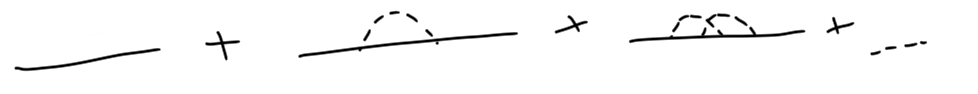
\includegraphics[scale=0.4]{images/lots.png}  \end{figure}

\noindent The end result if the sum of very many integrals of Wick contractions, and Feynman rules, dependent on the form of $\hat{H}_{int}$, are used to exploit patterns and cancellations in the terms. 

\subsection*{Example: Yukawa Theory}

\noindent Consider the Hamiltonian with interaction based on the fermion density $\hat{\bar{\psi}} \hat{\psi}$ and a single boson field $\hat{\phi}$, make the boson field sensitive to the density of the fermion field

\begin{equation}
\hat{H} =\hat{H}_{KG} + \hat{H}_{Dirac} + \int d^3 x \,\, g \, \hat{\bar{\psi}}(x) \hat{\psi}(x) \hat{\phi}(x).
\end{equation}

\noindent The Feynman rules in momentum space for this quantum field theory are, with dashed lines for bosons and solid lines for fermios

\begin{enumerate}
\item Propagators
	\subitem $\wick[offset=1.5em]{\c {\hat{\phi}(x)} \c {\hat{\phi}(y)}} = \frac{i}{p^2 - m_\phi^2 + i \epsilon} = $ \begin{figure}[H]\centering 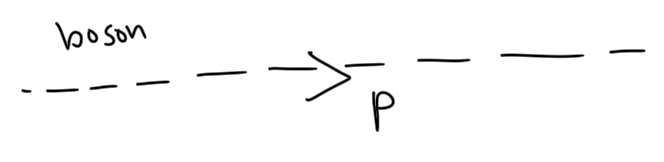
\includegraphics[scale=0.3]{images/bosonprop.png}  \end{figure}
	\subitem $\wick[offset=1.5em]{\c {\hat{\psi}(x)} \c {\hat{\bar{\psi}}(y)}} = \frac{i (\slashed{p} + m)}{p^2 - m^2 + i \epsilon} = $ \begin{figure}[H]\centering 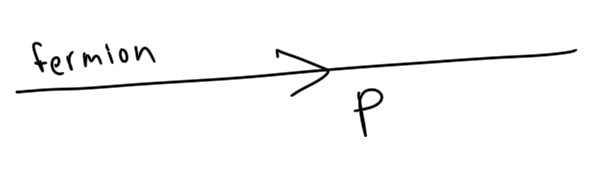
\includegraphics[scale=0.3]{images/fermionprop.png}  \end{figure}
\item Vertices
	\subitem $-ig = $ \begin{figure}[H]\centering 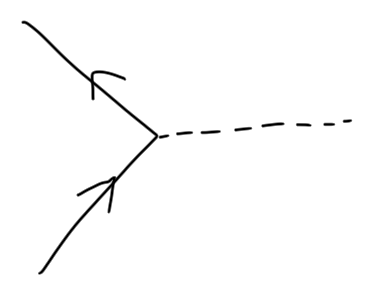
\includegraphics[scale=0.3]{images/vertex.png}  \end{figure}
\item External Legs
	\subitem $\wick[offset=1.5em]{\c {\hat{\phi}} \c {\ket{q}}} = 1 = $ \begin{figure}[H]\centering 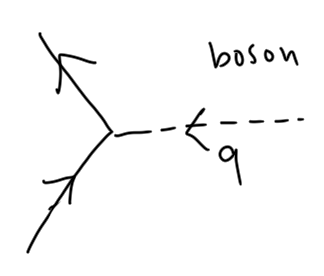
\includegraphics[scale=0.5]{images/bosonket.png}  \end{figure}
	\subitem $\wick[offset=1.5em]{\c {\bra{q}} \c {\hat{\phi}}} = 1 = $ \begin{figure}[H]\centering 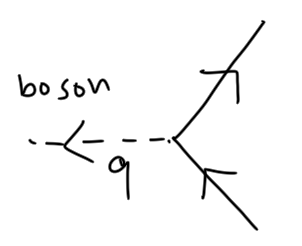
\includegraphics[scale=0.5]{images/bosonbra.png}  \end{figure}
	\subitem $\wick[offset=1.5em]{\c {\hat{\psi}} \c {\ket{p,s}}} = u^s (p) = $ \begin{figure}[H]\centering 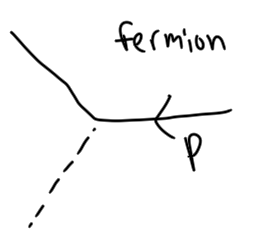
\includegraphics[scale=0.5]{images/fermionket.png}  \end{figure}
	\subitem $\wick[offset=1.5em]{\c {\bra{p,s}} \c {\hat{\bar{\psi}}}} = \bar{u}^s (p) = $ \begin{figure}[H]\centering 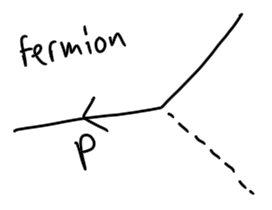
\includegraphics[scale=0.5]{images/fermionbra.png}  \end{figure}
	\subitem $\wick[offset=1.5em]{\c {\hat{\bar{\psi}}} \c {\ket{k,s}}} = \bar{v}^s (k) = $ \begin{figure}[H]\centering 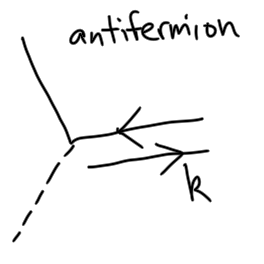
\includegraphics[scale=0.5]{images/antifermionket.png}  \end{figure}
	\subitem$ \wick[offset=1.5em]{\c {\bra{k,s}} \c {\hat{\psi}}} = v^s (k) = $ \begin{figure}[H]\centering 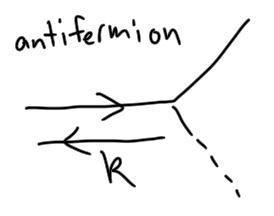
\includegraphics[scale=0.5]{images/antifermionbra.png}  \end{figure}
\item Conserve momentum at each vertex
\item Integrate over each loop momentum
\item Calculate the sign of the diagram
\item Divide by the symmetry factor
\end{enumerate}

\noindent Then the $n$-point Green's function is the sum of all connected and amputated Feynman diagrams with $n$ external legs subject to rules 1 through 7 above.

\noindent For example, a fermion scattering process looks like

\begin{figure}[H]\centering 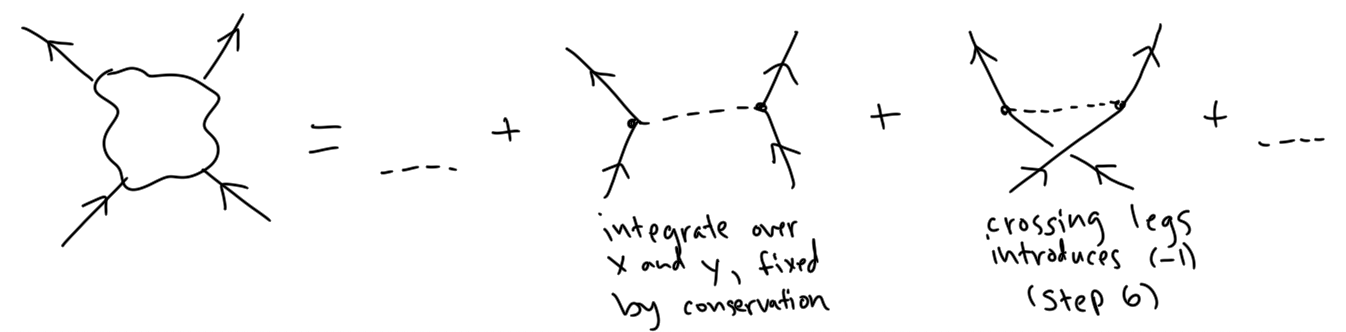
\includegraphics[scale=0.5]{images/fermionscattering.png}  \end{figure} 

\clearpage

\end{document}

